\documentclass{like}

%\selectlanguage{english}
%\selectlanguage{german}

\usepackage{amsmath}
\usepackage{pgfplotstable}
\usepackage{pgfplots}
\begin{document}



%%%%%%%%%%%%%%%%%%%%%%%%%%%%%%%%%%%%%%
%% Ab hier beginnt der Text
%%%%%%%%%%%%%%%%%%%%%%%%%%%%%%%%%%%%%%
  

%\normalsize
%Define our elements for our title page
\makeatletter

\renewcommand{\title}[1]{\gdef\@title{#1}}
\newcommand{\artderarbeit}[1]{\gdef\@artderarbeit{#1}}
\renewcommand{\author}[1]{\gdef\@author{#1}}
\newcommand\@matrikelnummer{\relax}
\newcommand{\matrikelnummer}[1]{\gdef\@matrikelnummer{#1}}
\newcommand{\professor}[1]{\gdef\@professor{#1}}
\newcommand\@studiengang{\relax}
\newcommand{\studiengang}[1]{\gdef\@studiengang{#1}}
\newcommand{\university}[1]{\gdef\@university{#1}}
\newcommand{\faulogo}[1]{\gdef\@faulogo{Abbildungen/#1}}
\newcommand{\likelogo}[1]{\gdef\@likelogo{Abbildungen/#1}}
\newcommand{\submitdate}[1]{\gdef\@submitdate{#1}}
\newcommand{\startdate}[1]{\gdef\@startdate{#1}}
\newcommand{\declaration}[1]{\gdef\@declaration{#1}}
\newcommand\@betreuerB{\relax}
\newcommand{\betreuerB}[1]{\gdef\@betreuerB{#1}}
\newcommand\@betreuerC{\relax}
\newcommand{\betreuerC}[1]{\gdef\@betreuerC{#1}}
\newcommand\@betreuerD{\relax}
\newcommand{\betreuerD}[1]{\gdef\@betreuerD{#1}}
 
%-----------------------------------------------------------------------
% Title page definition.
%-----------------------------------------------------------------------
\newcommand{\titlep}{
        \thispagestyle{empty}
        \begin{titlepage}
		\enlargethispage{4cm}
%        \null
		\vspace*{-2cm} 
        \begin{center}
{\rmfamily\large \textbf{ Friedrich-Alexander-Universität Erlangen-Nürnberg}}
\vskip 1,4cm
\begin{center}
%\includegraphics[scale=0.80, natwidth=1024, natheight=200]{\@faulogo} \hfill
\includegraphics[scale=0.80]{\@faulogo} \hfill
\vskip .8cm
{\large \bfseries Lehrstuhl für Informationstechnik\\(Schwerpunkt Kommunikationselektronik)}
\vskip 1.2cm
%\includegraphics[scale=0.40, natwidth=1024, natheight=200]{\@likelogo} \hfill
\includegraphics[scale=0.40]{\@likelogo} \hfill
\end{center}
\vskip .3cm
{\Large \@artderarbeit~mit dem Thema:\\}
\vskip 1.7cm
{\rmfamily\Large\bfseries\expandafter{\@title}}
        \end{center}
\vskip 1.5cm
		
\begin{table}[h!]
	\flushleft
%\setlength{\tabcolsep}{10pt}
	\large
\renewcommand{\arraystretch}{1,1}
	\begin{tabular}{p{4cm}l}
Bearbeiter     & {\rmfamily\large\expandafter{\@author}}\tabularnewline[.6ex]
\ifthenelse{\equal{\@matrikelnummer}{\relax}}{} {Matrikelnr. & \textrm{\@matrikelnummer}\tabularnewline[.6ex]}
\ifthenelse{\equal{\@studiengang}{\relax}}{}    {Studiengang & \textrm{\@studiengang}\tabularnewline[.6ex]}
Betreuer  & {\rmfamily\large\expandafter{\@professor}}\tabularnewline[.6ex]
                & \ifthenelse{\equal{\@betreuerB}{\relax}}{\vspace*{-0.6cm}}{\rmfamily\large{\@betreuerB}} \tabularnewline[.6ex]
                & \ifthenelse{\equal{\@betreuerC}{\relax}}{\vspace*{-0.9cm}}{\rmfamily\large{\@betreuerC}}  \tabularnewline[.6ex]
                & \ifthenelse{\equal{\@betreuerD}{\relax}}{\vspace*{-0.7cm}}{\rmfamily\large{\@betreuerD}} \tabularnewline[.6ex] Beginn         & {\rmfamily\large\expandafter{\@startdate}}\tabularnewline[.6ex]
Ende           & {\rmfamily\large\expandafter{\@submitdate}}            
	\end{tabular}
\end{table}
	        \vskip1cm
        \end{titlepage}
        \newpage}
        \makeatother
        
 


%-----------------------------------------------------------------------
% redefined \maketite
%-----------------------------------------------------------------------
\renewcommand{\maketitle}{%
                \titlep
	     }
%-----------------------------------------------------------------------
%  hier die eigenen Daten eintragen
%----------------------------------------------------------------------
    
\title{Modellfehler in optimierungsbasierter kombinierter Planung und Regelung für Rennwagen} % Mussfeld
\artderarbeit{Masterarbeit}         % Mussfeld
\author{Weller Sebastian}               % Mussfeld
\studiengang{Informations und Kommunikationstechnik}        % if Feld
\matrikelnummer{21777345}         % if Feld
\faulogo{fau.png}                   % Mussfeld
\likelogo{like.png}                 % Mussfeld
\professor{Prof. Dr.-Ing. Jörn Thielecke}       % Mussfeld
\betreuerB{Henrik Bey, M.\,Sc.}           % if Feld
%\betreuerC{Florian Particke, M.\,Sc.}              % if Feld
%\betreuerD{Betreuer D}             % if Feld  u.U. auskommentieren 
\startdate{08. Januar 2018}         % Mussfeld
\submitdate{09. Juli 2018}        % Mussfeld

% \maketitle

\maketitle
%BESTÄTIGUNG

\chapter*{Bestätigung}


\textbf{Erklärung:}\\

Ich versichere, dass ich die Arbeit ohne fremde Hilfe und ohne Benutzung anderer als der angegebenen Quellen angefertigt habe und, dass die Arbeit in gleicher oder ähnlicher Form noch keiner anderen Prüfungsbehörde vorgelegen hat und von dieser als Teil einer Prüfungsleistung angenommen wurde. Alle Ausführungen, die wörtlich oder sinngemäß übernommen wurden, sind als solche gekennzeichnet.
\vskip 2.5 cm
Erlangen, den (hier Datum eintragen)%{\rmfamily{\@submitdate}}
 \underline{\hspace{7cm} }
\vskip 1.5 cm

%DANKSAGUNG
%\pagestyle{scrheadings}
\chapter*{Danksagung}
%\headmark%chapter = Titel
%\section*{}
Ich möchte mich bei meinen Betreuern und meiner Familie bedanken.....

 %Optional
%Thema und Aufgabenstellung
 
%\pagestyle{scrheadings}

\chapter*{Thema und Aufgabenstellung}
\markboth{Thema und Aufgabenstellung}{Thema und Aufgabenstellung}
\textbf{Thema:}\par\smallskip

 Modellfehler in optimierungsbasierter kombinierter Planung und Regelung für Rennwagen

\textbf{Aufgabenstellung:}\par\smallskip
\par\smallskip  
Die Automatisierung des Fahrens schließt sowohl die Planung als auch die Regelung des Fahrzeugs mit ein. Häufig werden beide Bestandteile hierarchisch voneinander getrennt. Dies ist sinnvoll, solange das kontrollierte Fahrzeug sicher innerhalb der Aktuator\-li\-mi\-tie\-rungen betrieben werden soll, oder wenn die Trennung bereits durch die Problemstellung gegeben ist (Zieltrajektorie bereits vorgegeben) \cite{Williams2016AggressiveDW}.  

In anderen Fällen, z.B. wenn die gewünschte Dynamik wie in einer Rennsituation im Grenzbereich liegt, bietet sich eine kombinierte Planung und Regelung an. In diesem Beispiel würde die Kostenfunktion eine Minimierung der Rundenzeit beinhalten, während gleichzeitig die Beschränkungen des Fahrzeugs berücksichtigt werden.

Für derartige Probleme ist die modellprädiktive Regelung (MPC) bzw. eines ihrer Derivate besonders geeignet. Dabei kommt es immer zu einem sogenannten Modellfehler, der von der Komplexität und Genauigkeit des verwendeten Modells abhängt.

Das Ziel dieser Arbeit ist es, den Abfall bei der Leistung des Regelungsansatzes durch den Modellfehler zu untersuchen. Dafür soll eine Simulation verwendet werden.
Die Arbeit soll folgende Punkte beinhalten:
\begin{itemize}
\item Auswahl einer passenden Simulationsumgebung und deren Inbetriebnahme
\item Implementierung verschiedener (gegebener) Modelle für die Simulation
\item Implementierung des MPC-Ansatzes
\item Entwicklung einer einfachen Evaluationsmethode, um die Leistungsfähigkeit des Reglers zu untersuchen
\item Vergleich verschiedener Kombinationen aus Regler- und Simulationsmodellen
\end{itemize}
%Kurzzusammenfassung

\chapter*{Kurzzusammenfassung}

Mit zunehmender Rechenleistung und Erfahrung der Automobilbranche mit autonomen Fahrzeugen rückt auch das Thema der selbstfahrenden Rennautos immer mehr in den Fokus. Das ROBORACE Projekt ist hier Vorreiter mit seiner ausgefeilten Hardwareplattform und dem bereits in öffentlichen Events gezeigten Fahrleistungen. Auch die Formula Student (FS) verschließt sich nicht vor dem Trend und hat 2017 die Rubrik Driverless ins Leben gerufen. \\
Diese Masterarbeit beschreibt einen Ansatz zur Echtzeitregelung und Trajektionsplanung für ein eben solches Driverless-Racecar. Die Basis hierfür ist ein Model Predictive Control (MPC) Algorithmus. Er vereint die Regelung und Trajektionsplanung und ist sehr adaptiv bezüglich verschiedener Fahrsituationen und Ziele.
Als Ausgangssituation wird angenommen, dass das Fahrzeug bereits eine Runde auf einem unbekannten Kurs absolviert und nun eine genaue Karte des Kurses errechnet hat. 
Um das MPC nutzen zu können muss ein Fahrzeugmodell hinterlegt werden. Je genauer dieses ist, desto näher kann die Regelung an die Grenzen des realen Fahrzeuges gehen. Neben der Auslegung für das aktuellste FS-Fahrzeug des High Octane Motorsports für die Driverless Umrüstung, wird untersucht ab welchem Punkt ein kinematisches Modell nicht mehr ausreicht um das Fahrzeug sicher auf dem Rennkurs zu führen.



%\abstract 
\chapter*{Abstract}
In recent years with more and more computational power and sophisticated algorithms, autonomous cars are close to becoming a reality. An ancillary effect of this development is the emerging of driverless racecars. For this idea to become a reality, three key ingredients have to be met. A very good approximation of the location of the racecar in a virtual map, a trajectory planning algorithm and a controller that will drive the car on the computed path. In this thesis the model predictive control(MPC) algorithm is used, to combine the trajectory planning and controlling for an autonomous race car, build for the formula student driverless competition. A simulation environment will be developed to evaluate the effectiveness of the approach. One key part of this thesis is to investigate how prone to model errors the MPC-approach is and what performance can be expected for the use of a kinetic bicycle model as system description in the (MPC)-algorithm.
%%Abkürzungsverzeichnis
%\pagestyle{scrheadings}
%\chapter*{Abkürzungsverzeichnis}

\chapter*{Abkürzungsverzeichnis}
\addcontentsline{toc}{chapter}{Abkürzungsverzeichnis} %Abkürzungsverzeichnis kommt ins InhaV.





\begin{acronym}[SEPSEP] 
 \acro{Abk.}{Abkürzung}
 \acro{z.B.}{zum Beispiel}
 \acro{MPC}{Model Predictive Control}
 \acro{JIT}{just-in-time}
 \acro{SLSQP}{Sequential Least SQuarez Programming}
\end{acronym}


 (nach hinten verschoben)

\tableofcontents % erstelle hier das Inhaltsverzeichnis
\markboth{Contents}{Contents}
%\listoffigures % erstelle hier das Abbildungsverzeichnis 
%\listoftables % erstelle hier das Tabellenverzeichnis
\enlargethispage{2cm} %Bitte 2x kompilieren - sonst erscheint es nicht


\pagenumbering{arabic} %Seitennummerierung arabisch
\setcounter{page}{1}   %1. Kapitel soll mit Seitenzahl 1 beginnen
%------------------------------------------------------------------

\chapter{Einleitung}
Neben neu aufkommenden Trends in der Automobilindustrie, wie dem Elektroauto, Carsharing und dem aktuellen SUV-Boom, hat sich vor allem das autonome Auto in den letzten zwei Jahren mit dem Aufkommen von Teslas Autopilot stark in das Zentrum der Aufmerksamkeit von Firmen und Konsumenten bewegt. Das Jahr 2018 markiert dabei einen ganz besonderen Meilenstein. 
Ende des Jahres wird die Alphabet Tochter Waymo die ersten voll autonomen Taxis in Phönix für die Öffentlichkeit in Betrieb nehmen \cite{Waymo:1}. 
Dies ist jedoch nur möglich, da Google im gesamten Gebiet in dem sie ihren Service anbieten werden eine hochgenaue Umgebungskarte in den Fahrzeugen hinterlegt. Sollen die Fahrzeuge in unbekannten Umgebungen agieren, müssen sowohl die Sensorsysteme, wie auch die Algorithmen noch deutlich weiterentwickelt werden, bevor autonome Autos auf Stufe 5 frei verfügbar sind. Die Unterteilung dieser Level wurde von der Bundesanstalt für Straßenwesen zur Klassifizierung von selbst fahrenden Autos erstellt. Die Spanne geht von Stufe 0, keinerlei Assistenz beim fahren, bis Stufe 5, Vollautomatisierung. In diesen Fahrzeugen ist dann auch kein Lenkrad mehr vorgesehen. 
Die Forschung um dieses Ziel zu erreichen, wird nicht nur in den großen Automobilkonzernen betrieben. Bereits in der Schule aber vor allem an Universitäten und Hochschulen gibt es immer mehr Projekte an denen die Studenten sich intensiv mit der Entwicklung autonomer Roboter und Fahrzeugplattformen beschäftigen. Ein solches Projekt ist der Formula Student Driverless Wettbewerb.

\section{Formula Student Driverless}
Die Formula Student ist ein Ingenieurswettbewerb für Studenten. Er hat seine Wurzeln in den USA und wurde im Jahre 1981 das erste mal ausgetragen. Das Ziel des Wettbewerbes ist es, im Verlauf eines Jahres ein eigenes Rennauto zu konzipieren, designen, fertigen und sich schlussendlich mit anderen Teams zu messen. Dass der Wettbewerb sehr erfolgreich ist, machen nicht nur die inzwischen fast 700 Teams weltweit \cite{FsWorldRank:1} deutlich, sondern auch die Anzahl der verschiedenen Events, die überall auf der Welt im Sommer stattfinden. Seit dem Jahr 2017 gibt es neben der ursprünglichen Combustion-Klasse und der vor 10 Jahren eingeführten Electric-Klasse auch noch die Driverless-Klasse.
In dieser wird von den Teams ein Altfahrzeug mit Sensoren und Aktoren so erweitert, dass das Rennauto die Kurse autonom befahren kann.
Der Wettbewerb ist unterteilt in dynamische und statische Disziplinen. In letzteren werden verschiedene Präsentationen von den Teams verlangt. Diese beziehen sich auf die technische Realisierung, Softwaredesign, Kostenaufstellung und einen Businessplan.
Die dynamischen Disziplinen, in denen das Fahrzeug selbstständig fährt, sind:
\begin{itemize}
	\item Acceleration \\ Ein 75 Meter langer Beschleunigungsstreifen. Punkte werden nach der Zeit nicht nach der Endgeschwindigkeit vergeben.
	\item Skidpad \\ Eine liegende 8 bei der an der Engstelle eingefahren wird und jeweils zwei rechte und zwei linke Runden gefahren werden. Die zweite Runde geht jeweils in die Zeitmessung ein. Die Abmaße sind exakt vorgegeben.
	\item Trackdrive \\ Ein bis zu 800 Meter langer Kurs mit maximal 80 Meter langen Geraden und Kurven mit minimalem Innenradius von neun Metern. Es werden elf Runden gefahren und die Teams erhalten im Vornherein keine Möglichkeit Messungen am Kurs vorzunehmen.
\end{itemize}

Für die vorliegende Arbeit ist vor allem der Trackdrive von Interesse. Es wird davon ausgegangen, dass das Fahrzeug bereits die erste Runde absolviert und sich damit eine genaue Karte des Rennkurses erstellt hat. Die Messungen und Vergleiche beziehen sich damit auch immer auf einen Kurs, der so in einem FS-Event für die Driverless Fahrzeuge vorkommen könnte.

\begin{figure}[hb!]
	\centering
	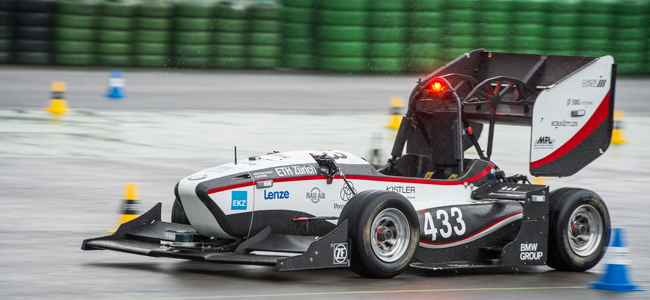
\includegraphics[width=270pt]{Abbildungen/amz-driverless-long.jpg}
	\caption{Zürichs FS-Driverless Fahrzeug im Jahr 2017 während des Trackdrive}
\end{figure}

\section{Problemstellung}
Im laufe dieser Arbeit soll ein Algorithmus entwickelt werden, der die Trajektionsplanung und Regelung eines Formula Student Driverless Racecars berechnet. Der dafür gewählte Ansatz ist \acl{MPC}. Es handelt sich dabei um ein Verfahren welches die Planung von Trajektorien und die Steuerung des Rennautos in einem Algorithmus vereint. Wie der Name schon sagt benötigt es hierfür ein Modell des zu kontrollierenden Systems mit dem daraufhin das zukünftige Verhalten vorausberechnet werden kann. Dieses Wissen wird genutzt um mit Hilfe einer Kostenfunktion die Steuerparameter so zu variieren, dass das Rennauto eine möglichst schnelle Rundenzeit erreicht.

\chapter{Stand der Technik}
Obwohl es zum Zeitpunkt der Arbeit noch keine öffentliche, autonome Rennserie außerhalb der Formula Student gibt, ist das Interesse an den dafür benötigten Technologien sehr groß.
Einen guten Rennfahrer zeichnet die Tatsache aus, dass er sein Fahrzeug in absoluten Grenzsituationen noch unter Kontrolle halten kann. Diese Eigenschaft ist nicht nur für autonome Rennautos wichtig, sondern ganz besonders auch für aktive Fahrassistenzsysteme. In kritische Fahrsituationen, in denen ein ungeübter Fahrer einen Unfall nicht mehr verhindern kann, können diese Systeme noch eingreifen. Um einen guten Rennfahrer in Software nachstellen zu können, müssen drei Grundvoraussetzungen geschaffen werden:
\begin{itemize}
	\item Genaue Kenntnis der Umgebung (dem Rennkurs) und der eigenen Position.
	\item Möglichst viel Wissen über das Verhalten des Fahrzeugs (Fahrzeugmodell).
	\item Kurze Reaktionszeiten (\emph{muscle memory}).
\end{itemize}

Um die Position des Fahrzeugs genau bestimmen zu können werden verschiedene Sensortypen mit Hilfe von Filterverfahren fusioniert. Die Genauigkeit der Schätzung steigt, im Vergleich zu den einzelnen Messsystemen, durch die Kombination signifikant an \cite{GPS_Fusion}, \cite{GPS_IMU_Fusion}. 
Um das Rennauto mit hoher Geschwindigkeit einen Rennkurs abfahren zu lassen, benötigt es ein Modell, welches das dynamische Verhalten des Fahrzeugs abbilden kann. Erst dieses Wissen ermöglicht die Berechnung von Trajektorien, welche das Rennauto an die Grenzen seiner Traktion bringt. Da die Modelle die  Fahreigenschaften nicht nur möglichst genau abbilden müssen, sondern auch schnell berechenbar sein müssen, werden verschiedene Vereinfachungen angewandt. Die Ansätze variieren nach Komplexität und zu bewältigenden Fahrsituationen:
\begin{itemize}
	\item Ein einfaches kinematisches Modell [\cite{MPC_Kinetic}], welches sehr schnell berechenbar ist, aber keine dynamischen Effekte berücksichtigt.
	\item Die Verwendung einer dynamischen Fahrzeugbeschreibung mit linearem oder nichtlinearem Reifenmodell [\cite{rc_car_1_43}, \cite{MPC_Dynamic}, \cite{MPC_Dynamic_Tire_Model}].
	\item Ein anderer Ansatz ist es, nicht vom Schwerpunkt des Autos aus die Fahrzeugdynamik zu berechnen, sondern den \emph{point of percussion} zu wählen. In diesem Punkt heben sich die rotatorischen und translatorischen Kräfte, hervorgerufen durch die Hinterreifen, gegenseitig auf \cite{CentreOfPercussion}.
\end{itemize}

Um ein mathematisches Fahrzeugmodell in einem realen Fahrzeug einsetzen zu können, müssen die Parameter, welche das System beschreiben möglichst genau bestimmt werden. Dies kann mit Hilfe einer linearen Regression sehr effizient und genau verwirklicht werden \cite{Williams2016AggressiveDW}. Die  Berechnungszeit für neue Steuerparameter sollte im Anwendungsfall eines autonomen Rennautos 40 bis 50 ms nicht überschreiten und bewegt sich in der Regel zwischen 50 und 100 Hz \cite{rc_car_1_43}, \cite{Williams2016AggressiveDW}. 
Sind die Grundvorraussetzungen geschaffen, gibt es unterschiedliche Ansätze ein Rennauto möglichst performant um einen Rennkurs fahren zu lassen. Eine Möglichkeit ist der Einsatz von neuronalen Netzen um geeignete Steuerparameter zu berechnen, wie vom Autor in \cite{6374146} beschrieben wurde. 
Ein "g-g`` - Ansatz, wie in \cite{KRITAYAKIRANA2010548}, nutzt ein Diagramm von lateralen(g) zu longitudinalen(g) Kräften, abhängig von verschiedenen Euler Spiralen um das Verhalten eines Rennfahrers zu Simulieren. Vor allem aber der in dieser Arbeit betrachtete \ac{MPC}-Algorithmus wird in einer Vielzahl von Arbeiten untersucht und verwendet. 
Die Unterschiede bei den Verfahren beziehen sich auf die getrennte Berechnung von Trajektorie und Regelung, Trennung von longitudinalem und lateralem Regler \cite{MPC_Dynamic}, \cite{MPC_Dynamic_Tire_Model} oder kombinierter Betrachtung \cite{rc_car_1_43}.


\chapter{Grundlagen}
Um für das Fahrzeug ideale Trajektorien zu berechnen und gleichzeitig das Rennauto in Echtzeit zu regeln wurde der Model Predictive Control Ansatz gewählt. Dieses Verfahren basiert auf der Optimierung eines nicht linearen Programms.
 
\section{Model Predictive Control}
Bei \ac{MPC} handelt es sich um einen Algorithmus, mit dem sich sehr komplexe, multivariable Regelungsprobleme lösen lassen. Er besitzt seine Stärken vor allem dort, wo Prozesse mit mehreren Ein-, und Ausgängen kontrolliert werden sollen und dabei verschiedene Beschränkungen eingehalten werden müssen. Vorausgesetzt es ist ein ausreichend genaues Modell des Prozesses vorhanden, können unter ausnutzen von Messungen und dem Modell zukünftige Zustände des Prozesses berechnet werden. Diese Information wird genutzt um die Eingangsparameter abhängig von dem gewünschten zukünftigen Verhalten des Prozesses, zu berechnen \cite{seborg2010process}. \\
Einige wichtige Vorteile von \ac{MPC} sind: 
\begin{itemize}
	\item Das sehr gute annähern an Prozessgrenzen und damit ein hoher Durchsatz/Effizienz.
	\item Einschränkungen der Eingangs- und Ausgangsgrößen werden berücksichtigt.
	\item Die Vorhersage des Fahrzeugzustands kann genutzt werden um mögliche Probleme frühzeitig zu detektieren.
\end{itemize}
Seit den späten 1970ern bis in die frühen 2000er wurde \ac{MPC} vor allem in der Chemiebranche genutzt um die komplexen multivariablen Regelungsprozesse , zum Beispiel in der Ölraffinerie, zu steuern. Für diese Aufgabengebiete war \acl{MPC} hervorragend geeignet, da die Prozesse im Vergleich zu anderen Regelungsaufgaben sehr langsam sind und damit die geringe Rechenleistung der damaligen Zeit ausreichend war. 
Gerade in den letzten Jahren, mit stark gestiegener Prozessorleistung, sind die Einsatzgebiete vielfältiger geworden. Auch die Steuerung hoch dynamischer Systeme wie Quadrocopter \cite{quadcopterMpc} oder Fahrzeugen \cite{carMPC} ist inzwischen möglich. 

\subsection*{Funktion}
Der systematische Ablauf eines \ac{MPC}- Algorithmus ist in Abbildung \ref{fig:mpcBlock} aufgezeigt.  

  \begin{figure}[ht!]
  	\centering
  	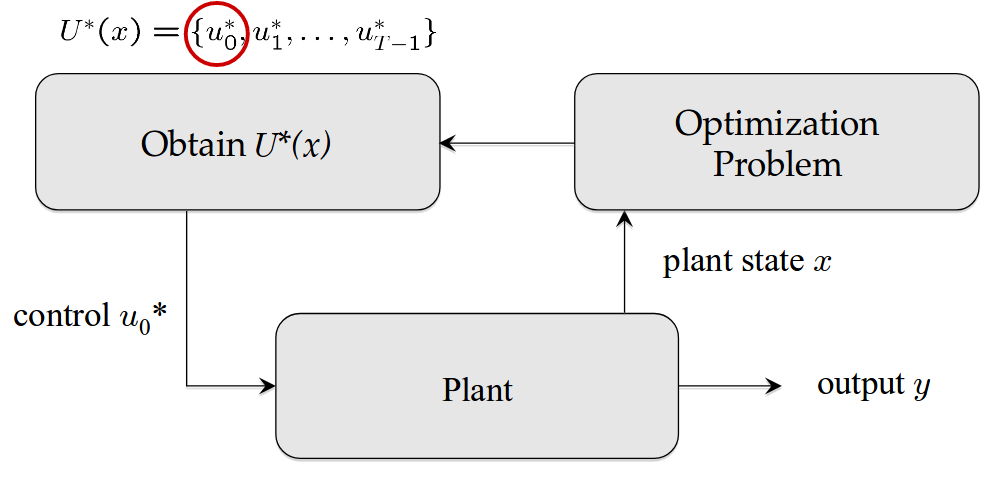
\includegraphics[width=350pt]{Abbildungen/mpcBlockDiagram.png}
  	\caption{Block Diagramm zu MPC}
  	\label{fig:mpcBlock}
  \end{figure}

Die Funktion lässt sich in drei Schritte unterteilen:
\begin{itemize}
	\item Zustandsschätzung \\ Im ersten Schritt wird der aktuelle Zustand des Systems erfasst und als Ausgangspunkt für die Berechnung des Optimierungsproblems festgelegt.
	\item Optimierung \\ In diesem Schritt werden die zukünftigen Zustände des Systems berechnet und welche Steuerparameter vonnöten sind um eine Kostenfunktion zu minimieren. Diese entspricht im industriellen Umfeld zum Beispiel einer Optimierung der Fertigungsrate, Kostenreduktion,  Temperatursteuerung, etc.
	\item Steuerung \\ Die berechneten Steuerparameter werden auf dem realen System angewandt. Danach wird wieder beim ersten Schritt fortgefahren.   
\end{itemize}


Die Mächtigkeit von \ac{MPC} basiert auf der Prädiktion des Systemverhaltens. Ein präzises Vorhersagen setzt daher eine möglichst gute Systembeschreibung voraus. Je genauer diese an die Realität heranreicht, desto weiter in die Zukunft können die Systemzustände berechnet werden. Zudem kann das System näher an seine Systemgrenzen geführt werden. \\
Bei \acl{MPC} handelt es sich um ein sogenanntes \textit{finite-horizon} Verfahren, das heißt, die Optimierung wird immer für einen bestimmten Zeitraum in die Zukunft durchgeführt $ [t_0, t_0 + T] $. Dieser Bereich \(T\) wird dann in \(k\) Schritte unterteilt, für die jeweils ein Prädiktionsschritt berechnet wird. Dieser geht aus dem vorherigen Zustand $k -1$ und den dazu gehörigen Steuergrößen hervor. Nachdem der Optimierer die für eine Kostenfunktion idealen Steuergrößen für den gesamten Prädiktionsvektor berechnet hat, wird nur der \emph{erste} Steuerwert ausgewählt und zur Regelung im realen System eingesetzt. Der Zusammenhang aus Prädiktion und Kostenfunktion ist im Schaubild \ref{fig:mpcTheory} verdeutlicht. Für jeden Schritt im Vorhersage Horizont wird der Steuerparameter berechnet, welcher den Systemzustand möglichst schnell der vorgegebenen Trajektorie annähert. Das wissen über das zu steuernde System hilft dafür die passenden Steuerparameter zu finden und frühzeitig genug die Amplitude so anzupassen dass kein Übersteuern entsteht. Es wird also deutlich, dass ein \ac{MPC}-Algorithmus sehr gut an die Systemgrenzen regeln kann.

\begin{figure}[ht!]
	\centering
	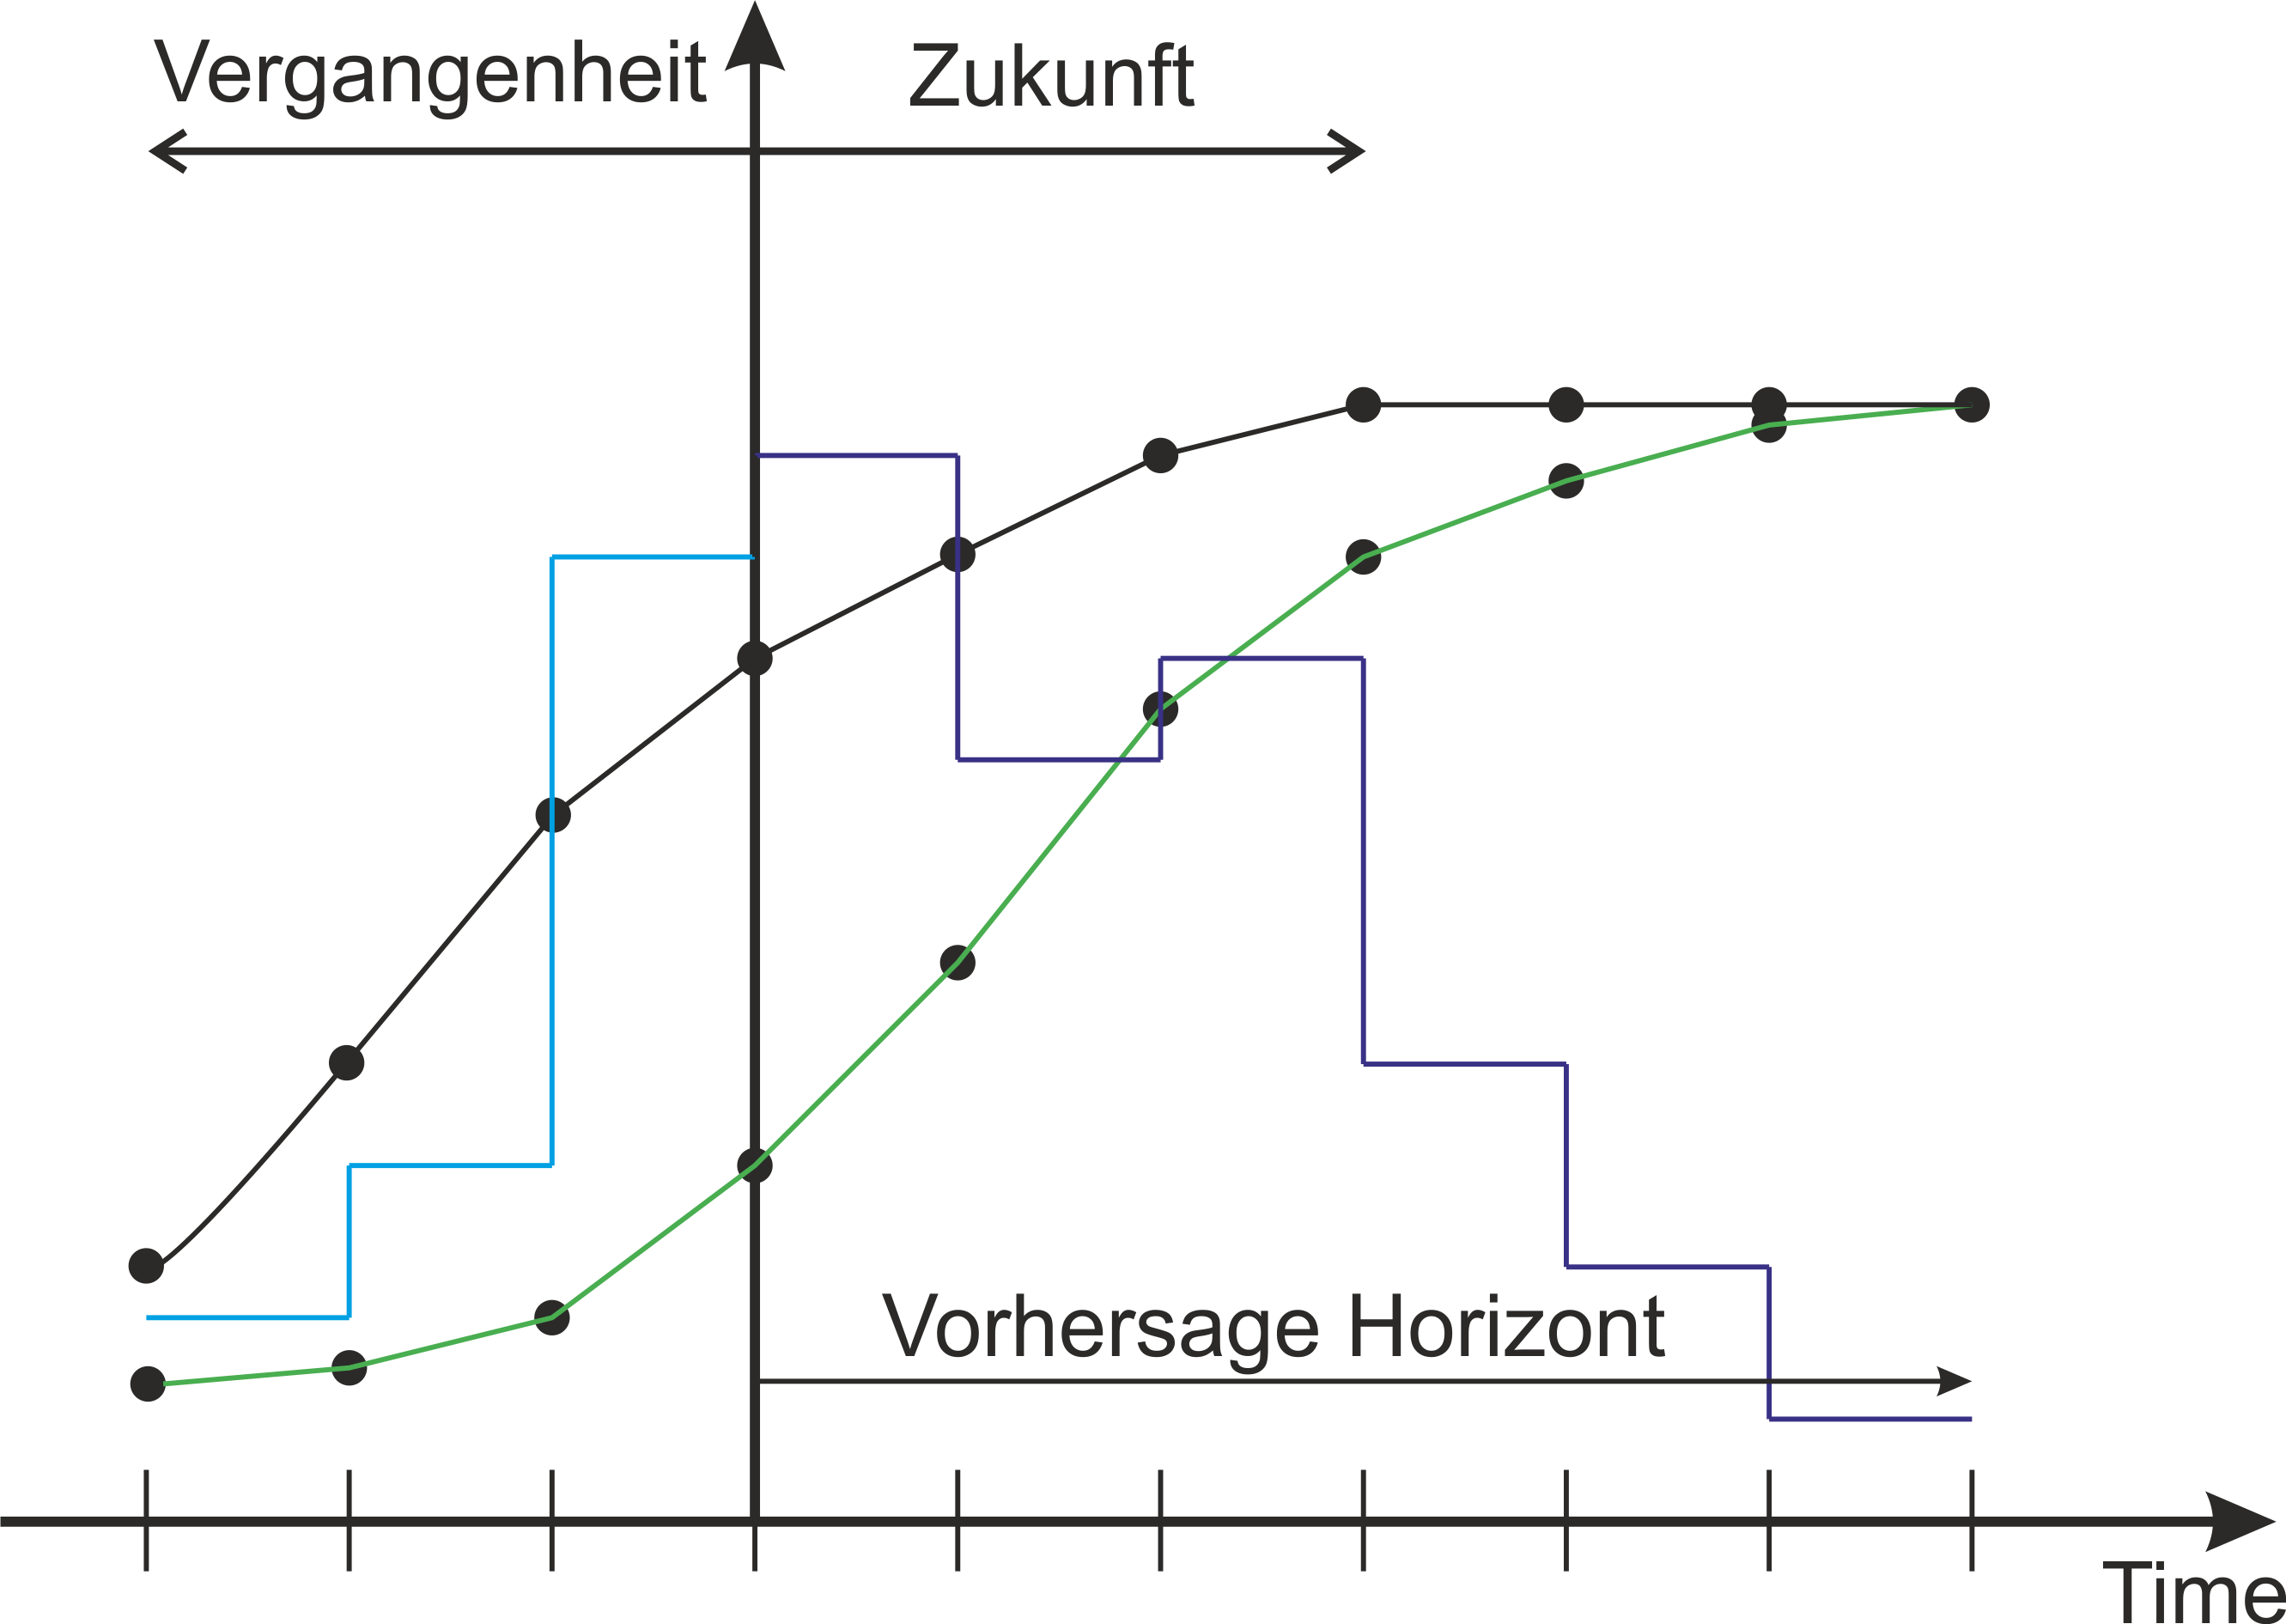
\includegraphics[width=350pt]{Abbildungen/mpcParadigm.png}
	\caption{Funktionsprinzip von \ac{MPC}: Die Kostenfunktion ist die Reduktion der Distanz zur Referenztrajektorie. Durch das Modell kann das System so geregelt werden dass es nicht über die Zieltrajektorie hinaus schießt.}
	\label{fig:mpcTheory}
\end{figure}

Wie bereits ausgeführt wurde, berücksichtigt der \ac{MPC}-Ansatz auch Eingangs-, Ausgangs- und Zustandsbeschränkungen mit welchen man den Suchraum einschränkt. Diese sind im Falle eines Rennautos zum Beispiel die maximale Geschwindigkeit, Lenkeinschlag, Beschleunigung und Bremskraft. Ebenfalls ein sehr gutes Beispiel für eine Zustandsbeschränkung ist die Änderungsrate der Querbeschleunigung, welche ein direkter Indikator für den Komfort eines autonomen Fahrzeugs während der Fahrt darstellt.\\

Um den \textit{\acl{MPC}} Algorithmus für den Anwendungsfall eines Rennautos zu implementieren, braucht man Folglich ein Fahrzeugmodell und einen Optimierungsalgorithmus. Auf beides wird in den nächsten Kapiteln eingegangen.


\section{Optimierung}
Das Konzept der Optimierung besteht darin, eine gegebene Funktion \(f(\vec{x})\), auch als Kostenfunktion bezeichnet, zu mini- oder zu maximieren. 
Dies wird in einer Vielzahl von Anwendungsgebieten genutzt.
Zur Berechnung von Profit / Verlust in einem Betrieb, Geschwindigkeit oder Distanz in einem physikalischen Problem oder der erwartete \textit{return of investment} für eine Geldanlage.  
Die Bezeichnung lineare Programmierung bezieht sich auf die Lösung eines  Optimierungsproblems und hat nichts mit dem eigentlichen Programm zu tun.

Die allgemeine mathematische Definition eines Optimierungsproblems ist

$minimize$  
\noindent\hspace*{3mm}%
$f(\vec{x}) $ \\
$subject$  $to$ 
\noindent\hspace*{3mm}%
$g_i(\vec{x})$ $\leq$ $0,$ $i=1,2,...,p$  \\
\noindent\hspace*{22mm}%
$h_j(\vec{x})= 0,$ $j= 1,2,...,m$\\ 
\noindent\hspace*{22mm}%


Der Eingabeparameter $\vec{x}$ sei aus $\Re \textsuperscript{n} $, das heißt, das Problem hängt von \(n\) Einflussparameter ab, die im Vektor $\vec{x}$ eingelagert sind. Die Zielfunktion $f:D \rightarrow \Re $ sei einmal stetig differenzierbar. Weiterhin sind die Nebenbedingungen in Ungleichheitsform $g_i:D \rightarrow \Re$ mit $1\leq i \leq p$ und in Gleichheitsform $h_j:D \rightarrow \Re$ mit $1\leq j \leq m$ gegeben.
Wird \(f(\vec{x})\) durch \(-f(\vec{x})\) ersetzt, wird aus dem Mini-, ein Maximierungsproblem.  

Ein Optimierungsproblem hat nicht immer eine Lösung. Die Ungleichungen, welche den Suchraum einschränken, können sich widersprechen (z.b. $x \leq 0 $ und $x > 0$). In diesem Fall gibt es keine Lösung. Außerdem kann das Problem unbeschränkt sein, was unendlich viele zulässige Lösungen zur Folge hätte und damit auch als nicht lösbar eingestuft wird. 

Ein lineares Programm (alle Funktionen sind linear) lässt sich in Matrixschreibweise darstellen. Es besteht aus $A \in \Re \textsuperscript{m,n}$ und zwei Vektoren $b \in \Re \textsuperscript{m,1}$ und $c \in \Re \textsuperscript{1,n}$. \\

\[ \left( \begin{array}{cccc}
a_{11} x_1 + & ... & + a_{1n} x_n & \leq b_1 \\   	
a_{21} x_1 + & ... & + a_{2n} x_n & \leq b_2 \\ 
. & . & . & . \\
. & . & . & . \\
a_{m1} x_1 + & ... & + a_{mn} x_n & \leq b_m \\
\end{array} \right)\] 

Das Optimierungsverfahren sucht eine Lösung für den Vektor \(\vec{x}\) welcher sowohl die linearen Bedingungen erfüllt, als auch die Zielfunktion 
$cx=c_1 x_1 + ... + c_n x_n$ minimiert.
Die Kurzschreibweise für dieses Gleichungssystem ist: \\
$min \{ c\textsuperscript{T}x | Ax \leq b, x \geq 0 \}$

Besonders einfach veranschaulichen lässt sich die Lösung des Problems geometrisch im zweidimensionalen Raum, so dargestellt in Abbildung \ref*{fig:linOpt}.

\begin{figure}[ht!]
	\centering
	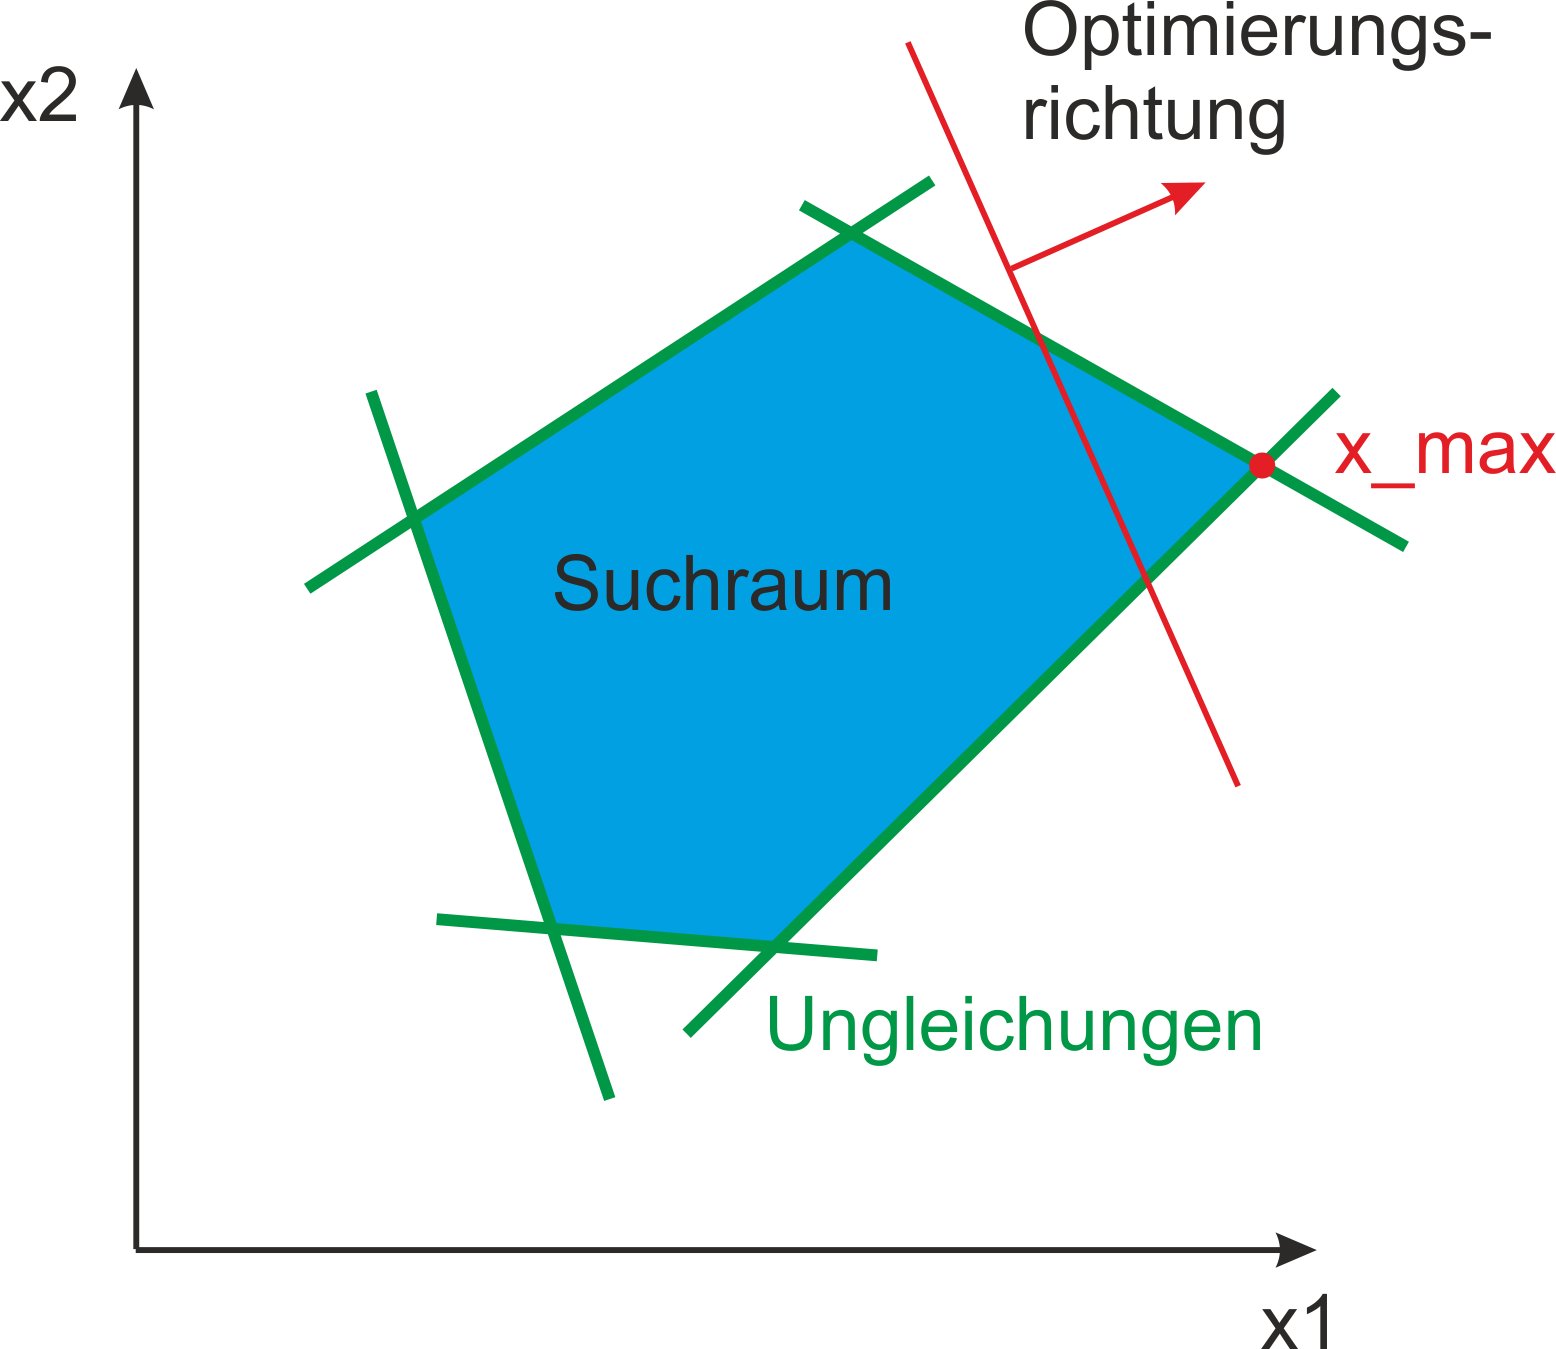
\includegraphics[width=300pt]{Abbildungen/linearOpt.png}
	\caption{Lineare Optimierung}
	\label{fig:linOpt}
\end{figure}

Jede Ungleichung $a_i x \leq b_i$ teilt den Suchraum in zwei Hälften, eine mit zulässigen Punkten und eine ohne. Die Punkte auf der Grenze sind ebenfalls zulässig. Die Menge der Punkte welche alle Ungleichungen erfüllt, ist genau der Schnitt dieser Halbräume. Dieser Bereich ist in Abbildung \ref{fig:linOpt} blau dargestellt. Der Punkt, der die Kostenfunktion $c: x \rightarrow c\textsuperscript{T} x$ minimiert, liegt auf den Kanten der Ungleichungen und wird durch Verschiebung der Hyperebene $ \{x| c\textsuperscript{T} x = 0 \}$ in Richtung des Vektors \(c\) gefunden. Nachdem das Optimierungsproblem aufgestellt ist, gibt es verschiedene Ansätze dieses zu berechnen.


\subsection*{Lösungsverfahren}

\subsection{Simplex - Verfahren}
Bei der in dieser Arbeit zu lösenden Optimierung, handelt es sich um ein nichtlineares Problem. Um ein besseres Verständnis für das Lösungsverfahren zu bekommen, welches hierfür genutzt wird, soll zuerst das Simplex-Verfahren kurz vorgestellt werden. Das Verfahren wurde 1947 von Dantzig \cite{dantzig51} entwickelt und nutzt die Eigenschaft, dass ein \textit{well behaved} (wenn das aufgestellte Problem der Standardform entspricht und lösbar ist) lineares Programm immer einen Knoten besitzt an dem sich Kanten verschiedener Ungleichheitsbedingungen treffen und die Kostenfunktion minimieren. Das Verfahren nutzt diesen Zustand aus, in dem es sich iterativ von einem Eckpunkt zum nächsten bewegt. 
\begin{figure}[ht!]
	\centering
	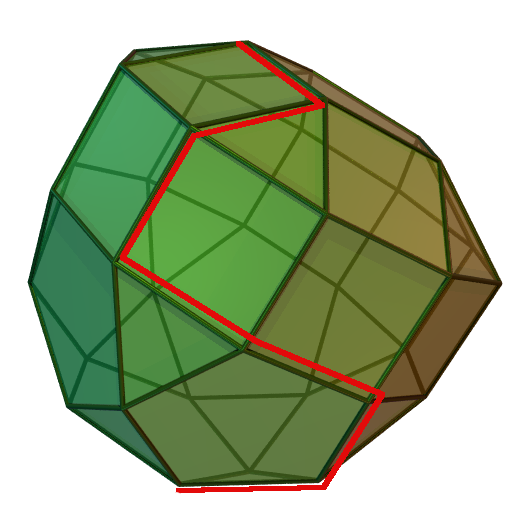
\includegraphics[width=200pt]{Abbildungen/simplexMethod.png}
	\caption{Simplex Methode: Ablaufen des Suchraums entlang der Kanten der Ungleichheitsbedingungen von Knoten zu Knoten}
	\label{fig:splxMethod}
\end{figure}

Die Richtung, welche gewählt wird, hängt von der Flanke (Ungleichung) ab, welche die Kostenfunktion weiter minimiert. Kann keine weitere Flanke gefunden werden, welche die Kosten weiter reduziert, endet das Verfahren im Optimum. Da im schlechtesten Fall der Simplex-Algorithmus jeden Knotenpunkt einmal besuchen muss, hat das Verfahren ein exponentielles Wachstum $\mathcal{O}(c\textsuperscript{n})$, abhängig von der Dimension des Optimierungsproblems \cite{doi:10.1137/S0036144502414942}.Trotz dieser Problematik hat das Simplex-Verfahren in der Praxis eine sehr gute Laufzeit und kann für den wiederholten Aufruf einer nur leicht veränderten Optimierung (anpassen von Parametern nach dem letzten Aufruf) einen sogenannten Warmstart nutzen. Dieser beschleunigt die Lösung ebenfalls deutlich \cite{simplexWiki:1}.\\
Die Suche nach noch besseren Verfahren, dessen Komplexität nur polynomial mit der Dimension anwächst, führte dann in den Jahren 1979 bis 1984 zur Entwicklung eines neuen Algorithmus, welcher auch für nichtlineare Probleme genutzt werden kann.

\subsection{Innere-Punkte-Verfahren} 
\label{ipm} 
Im Folgenden wir das Innere-Punkte-Lösungsverfahren für lineare, quadratische und nichtlineare Optimierungsprobleme kurz vorgestellt. Die Idee hinter dem Verfahren ist es, sich nicht mehr auf den Kanten zu bewegen, sondern immer im Inneren des erlaubten Bereiches. Diese Bewegung durch das Innere des Polytop ist in Abbildung \ref{fig:iterPointMethod} veranschaulicht.  
\begin{figure}[ht!]
	\centering
	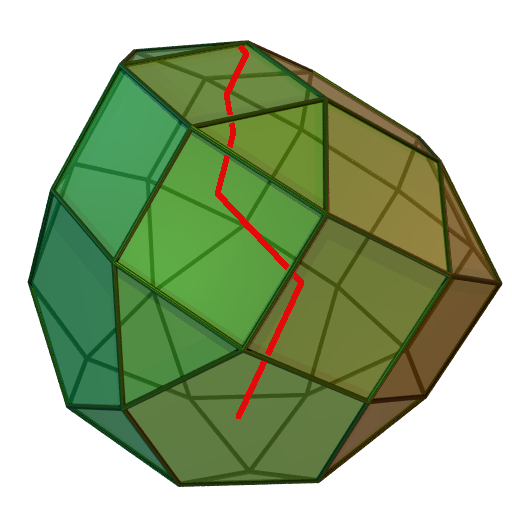
\includegraphics[width=200pt]{Abbildungen/iterPointMethod.png}
	\caption{Beim Innere-Punkte-Verfahren bewegt sich der Optimierer durch das Innere des Polytop auf der Suche nach dem Mimimum.}
	\label{fig:iterPointMethod}
\end{figure}

Um dieses Verfahren umzusetzen wird die Positivitätsbedingungen $x \geq 0$ der Standardform durch einen logarithmische Strafterm $-\mu \ln x_i $  ersetzt und in die Kostenfunktion integriert. 
Der Faktor $\mu$ wird genutzt um die Gewichtung des Strafterms zu verändern.
Die daraus resultierende Funktion wird als Barrierefunktion bezeichnet und ist definiert als \\
$B(x,\mu) =  c\textsuperscript{T}x - \mu \sum_{i}^{n} \ln x_i$, mit $\mu > 0$. \\
Das ursprüngliche Optimierungsproblem wird damit ersetzt durch 
$min \{B(x,\mu) | Ax \leq b\}$.\\
Wird \(\mu\) sehr klein (tendiert gegen \(0\) ) ist die Lösung des Barriereproblems die gleiche wie unser ursprüngliches Optimierungsproblem. Dies nutzt man aus, um von einem großen \(\mu\) als Startpunkt iterativ $B(x,\mu)$ zu optimieren und dann vor der nächsten Iteration \(\mu\) zu verkleinern.

Für kleine Werte von x wird $-\ln x $ sehr groß. Dies nutzt man aus, um kleine Werte von \(x\) zu bestrafen und damit die Suche der Lösung immer innerhalb des zulässigen Bereiches zu führen (verdeutlicht in Abbildung \ref{fig:iterPointMethod}). Während der Suche wird \(\mu\) sukzessive verkleinert, bis im Grenzfall $ \mu \rightarrow 0$ das Barriereproblem gegen die Lösung des Optimierungsproblems konvergiert (siehe Abbildung \ref{fig:iterPointLn}).\\

\begin{figure}[ht!]
	\centering
	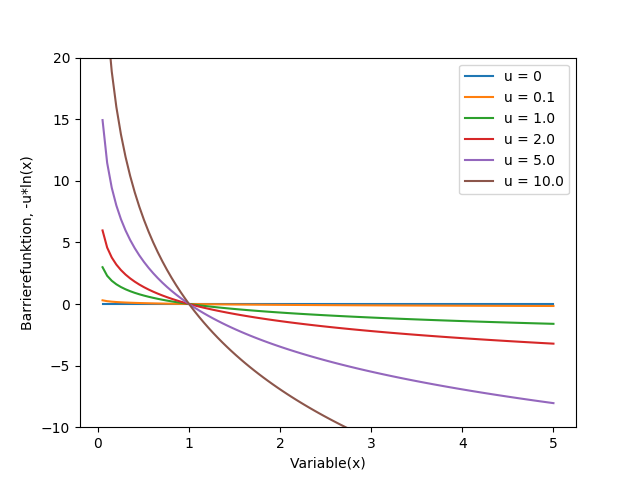
\includegraphics[width=350pt]{Abbildungen/intPointLn.png}
	\caption{Logarithmische Barrierefunktionen}
	\label{fig:iterPointLn}
\end{figure}

Um in jedem der iterativen Schritte möglichst schnell zu einer Lösung zu kommen, bedient man sich dem Newton-Rapshon-Verfahren. 
Der Algorithmus benötigt die Ableitungsmatrix der Barrierefunktion. Die Berechnung dieser wird durch eine automatische Ableitung realisiert.

\subsection{Automatische Ableitung} 

Ableitungen sind eine Grundvoraussetzung für viele numerische Algorithmen. Die Genauigkeit der Berechnung und die Geschwindigkeit sind jedoch oftmals problematisch.

Ein möglicher Ansatz die Ableitung $\Delta{\tiny } f(x) = (\frac{\partial f}{\partial x_1} (x), ..., \frac{\partial f}{\partial x_n})$ der Funktion $f:\Re \textsuperscript{n} \rightarrow \Re $ zu berechnen ist \\
$f'(x) \approx \frac{f(x+h) - f(h)}{h}$ mit $ h \rightarrow 0 $. \\
Dieser Ansatz ist jedoch nicht nur sehr ineffizient $\mathcal{O}(n)$, sondern besitzt zudem noch Rundungsfehler \cite{julDiff}.
Eine andere Möglichkeit wäre die Ableitung manuell zu berechnen, was jedoch für komplexere Systeme sehr aufwendig und vor allem fehleranfällig ist. Eine bessere Lösung ist die automatische Ableitung (\emph{automatic differentiation}). 
Dieses System kann die Ableitung bis auf die maximal mögliche Genauigkeit eines \textit{float}-Datentyp berechnen. Zu der höheren Präzision kommt noch die deutlich bessere Laufzeit. Im Idealfall entspricht die Komplexität $\mathcal{O}(1)$ \cite{julDiff}. Um diese Vorteile nutzen zu können, benötigt es jedoch ein genaues Wissen über die abzuleitende Funktion \(f(x)\). Realisiert wird dies durch den Zugriff auf den Sourcecode der Methode oder durch ein überladen der Operatoren. Das Verfahren ist abhängig von den Möglichkeiten der Programmiersprache und welcher Ansatz bei der Implementierung der automatischen Ableitung verfolgt wurde. 


\subsubsection*{Vorwärtsmodus}
Ein Verfahren der Umsetzung ist der Vorwärtsmodus. Er basiert auf der Kettenregel $(f \circ g)' = (f' \circ g)g'$. \\
Um dies auszunutzen wird eine abzuleitende Funktion $ y = f(g(h(x)))$ in seine Bestandteile $y = f(g(h(w_0))) = f(g(w_1)) = f(w_2) = w_3$ aufgetrennt und anschließend in die Kettenregel eingesetzt. 

$\frac{\partial y}{\partial x} = \frac{\partial y}{\partial w_2} \frac{\partial w_2}{\partial w_1} \frac{\partial w_1}{\partial x}$. \\
Zum besseren Verständnis wird die Ableitung für folgende Funktion
$y = f(x_1, x_2) = x_1x_2 + \sin(x_1)$ berechnet.\\
Dazu werden wie oben bereits beschrieben zuerst die Bestandteile substituiert:\\
$y = w_1w_2 + \sin(w_1) $ \\
$y = w_3 + w_4$ \\
$y = w_5$

Danach muss der sogenannte \textit{seed} errechnet werden. Er kodiert über welche Variable differenziert werden soll. Für $x_1$ ist der \textit{seed} $\dot{w_1} = \frac{\partial x_1}{\partial x_1} = 1$ und   $\dot{w_2} = \frac{\partial x_2}{\partial x_1} = 0$
Im letzten Schritt werden nur noch von innen nach außen die Substitutionen ersetzt. \\
$\dot{w_3} = w_2\dot{w_1} + w_1 \dot{w_2}$ \\
$\dot{w_4} = \cos{w_1} \cdot \dot{w_1}$ \\
$\dot{w_5} = \dot{w_3} + \dot{w_4}$ \\
Dieses Verfahren kann im sogenannten Rückwärtsmodus auch von außen nach innen berechnet werden. Nachdem die Grundlagen zur Optimierung gelegt wurden, wird nun auf den Teil im \acl{MPC} eingegangen, welcher die Un- und Gleichheitsbedienungen definiert. 


\section{Fahrzeugmodelle}

Wie der Name Model Predictive Control schon verdeutlicht benötigt man eine Systembeschreibung des zu regelnden Modells. Diese wird genutzt, um zukünftige Zustände zu berechnen und bildet damit einen wichtigen Bestandteil. Desto genauer die Beschreibung das reale System approximiert, desto besser ist die Vorhersage und damit auch die Regelung des Fahrzeugs.
Im Folgenden wird zuerst ein kinematisches Fahrzeugmodell eingeführt und dann zu einem dynamischen Modell erweitert.   

\subsection{Kinematisches Modell}
\label{kinematicModel}
Unter gewissen Einschränkungen, welche weiter unten beschrieben werden, kann ein kinematisches Modell die laterale und longitudinale Bewegung eines Fahrzeuges mathematisch beschreiben. In diesem sehr stark vereinfachten Modell werden keine wirkenden Kräfte berücksichtigt, sondern nur die geometrischen Beziehungen des Fahrzeuges genutzt, um die Bewegung zu berechnen. \\
Im ersten Schritt werden die jeweils an einer Achse verbundenen Räder zu einem einzigen zusammengefasst. Dies wird als Bicycle Modell bezeichnet und vereinfacht die Berechnungen erheblich \cite{BicycleModel}. Obwohl auch für Hinterradlenkung möglich, wird im Folgenden nur die Vorderradlenkung betrachtet. Die Lenkwinkel, welche durch das Bicycle Modell berechnet werden, entsprechen nicht den Lenkwinkeln am echten Fahrzeug. Die kurveninneren und kurvenäußeren Räder bewegen sich auf zwei Kreisen mit unterschiedlichen Radien und damit auch verschiedenen Anstellwinkeln. Dies wird in Fahrzeugen durch die Ackermann Lenkung mechanisch umgesetzt \cite{rajamani2011vehicle}.


Die nichtlinearen, zeit kontinuierlichen Gleichungen basieren auf \cite{rajamani2011vehicle, 7225830} und beschreiben das kinematische Modell bezüglich eines Inertialsystems (siehe Abbildung \ref{fig:kinmodel}),

\begin{figure}[ht!]
	\centering
	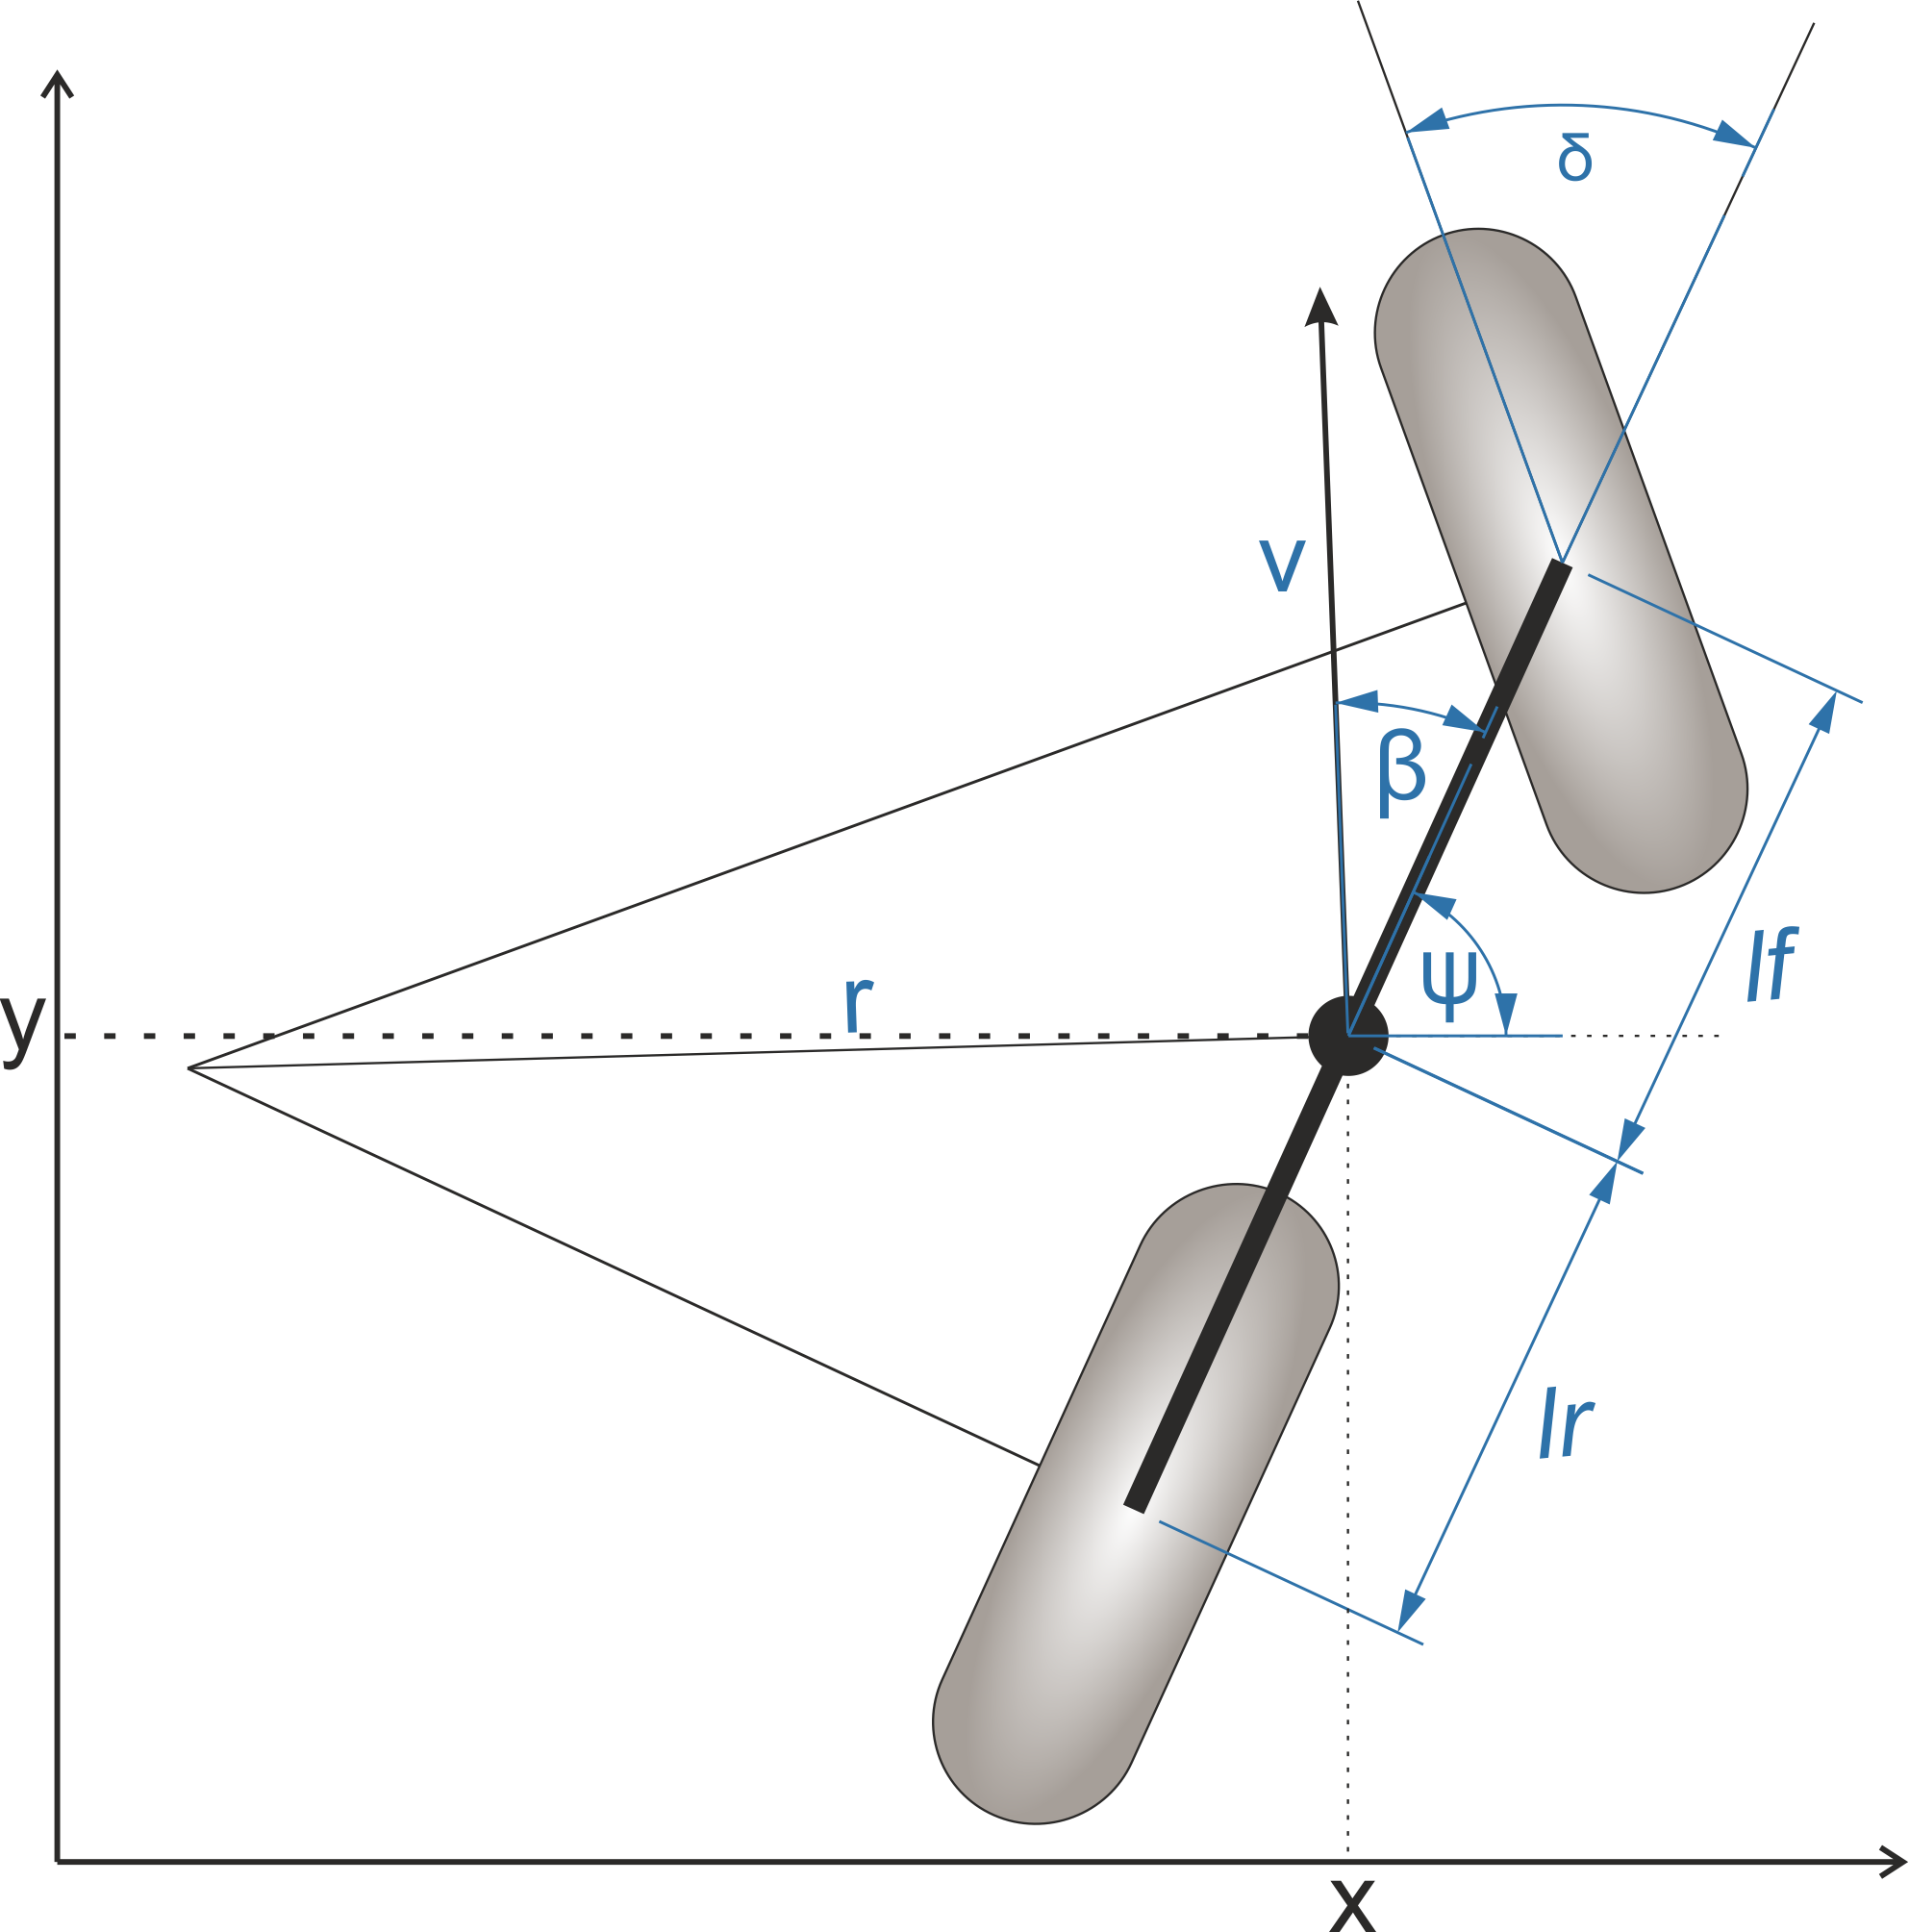
\includegraphics[width=250pt]{Abbildungen/kinBicycle.png}
	\caption{Kinematisches Modell:}
	\label{fig:kinmodel}
\end{figure}

\begin{eqnarray}
\label{kinDiscrete}
\dot{x}   &= &v  \cos(\psi + \beta)\\
\dot{y}   &= &v  \sin(\psi + \beta)\\
\dot{\psi} &= &\frac{v}{l_r} \sin(\beta) \\
\dot{v}    &= &a \\
\beta      &= &\arctan(\frac{l_r}{l_f + l_r} \tan(\delta_f))
\end{eqnarray}

in dem \(x\) und \(y\) die Koordinaten des Schwerpunktes im Inertialsystem darstellen. 
\(\varphi\) ist die Orientierung und \(v\) die Geschwindigkeit des Fahrzeugs. \(l_f\) und \(l_r\) sind die Abstände der vorderen (\(l_f)\) und hinteren (\(l_r)\) Achsen zum Schwerpunkt.
Der Schwimmwinkel (\(\beta\)) ist der Winkel  zwischen der Bewegungsrichtung des Fahrzeugs im Schwerpunkt und der Fahrzeuglängsachse bei der Kurvenfahrt. Die Beschleunigung \(a\) bezieht sich ebenfalls auf den Schwerpunkt und zeigt immer in die gleiche Richtung wie auch die Geschwindigkeit. \\
Die Parameter lassen sich in zwei Bereiche unterteilen:

\begin{itemize}
	\item Steuerparameter  \\
	\(a\), \(\delta\)
	\item Zustandsgrößen \\
	\(x\), \(y\), \(v\), \(\psi\)
	
\end{itemize}


Die Annahme eines kräftefreien Modells, bei dem das Vorderrad genau in die Richtung rollt in die es zeigt, ist nur bis etwa 5 m/s plausibel \cite{rajamani2011vehicle}. Danach müssen die Kräfte, welche die Reifen auf die Straße übertragen können mit betrachtet werden. Diese werden dann im dynamischen Modell genutzt, um eine genauere Vorhersage berechnen zu können.

Die für das kinematische Modell angenommenen Werte stammen vom Fahrzeug aus dem Jahr 2017 des High Octane Motorsports Verein (siehe \ref{vehicleParam}). Die Beschleunigung \(a\) wurde für den besten \textit{Acceleration} Durchgang in FSG-2017 mit der Zeit $t = 4.5s$ und der Endgeschwindigkeit $v = 32.78 \frac{m}{s\textsuperscript{2}}$ berechnet. Für 
\begin{equation}
a = \frac{v}{t}  \label{long_acc_kin}
\end{equation}
erhält man eine mittlere Beschleunigung von $7.284 \frac{m}{s\textsuperscript{2}} $.

Überprüft man die Werte mit der Formel zum Berechnen der zurück gelegten Entfernung 
\begin{equation}
x = \frac{1}{2} * a * t^2  
\end{equation}
liegt man mit \(73.75m\) nur zwei Prozent neben der genauen Streckenlänge von \(75m\).

\subsubsection*{Begrenzung des Kurvenradius}
\label{betaMax}
Da beim kinematischen Modell die Geschwindigkeit in Kurven keine Rolle spielt, kann das Fahrzeug mit jedem \(v\) den gleichen Kurvenradius durchfahren. Um auch in höheren Geschwindigkeiten eine akzeptable Regelung zu erhalten wird eine Beschränkung eingefügt, welche die maximale Querbeschleunigung beschränkt. Der Maximalwert entspricht dem höchsten g-Wert den das Fahrzeug des High Octane Motorsports mit Aerodynamik in einer Kurve erreichen kann: $a_{max} = 2.0g$. 
Mit der Gleichung
\begin{equation}
	|\beta| \leq \arctan(\frac{1}{2} \frac{\frac{l}{2} a_{max}}{v^2})
\end{equation}
wird dies über die Einschränkung des Schwimmwinkel (und damit gleichzeitig des Lenkwinkels) erreicht.


\subsection{Reifenmodell}
\label{tireModel}
Da der Reifen der einzige Kontaktpunkt zwischen Fahrbahn und Fahrzeug ist,  beeinflussen er das Fahrverhalten maßgeblich. Aufgabe des Reifens ist es, sämtliche Kräfte und Momente zu übertragen, um eine optimale Straßenlage zu erzielen. Demzufolge ist der Reifen das Bauteil, welches die Fahrleistungen am stärksten einschränkt.

Die Kräfte, welche ein Reifen auf die Straße übertragen kann, hängen von dem Schräglaufwinkel, Schlupf und der Radlast ab. Die Radlast \(F_z\) berechnet sich aus der Normalkraft und der Radlastverteilung und wird im folgenden als konstant angesehen.
Die Seitenführungskraft \(F_y\) wirkt bei einer Kurvenfahrt der Fliehkraft entgegen und hält das Fahrzeug auf der Spur solange ein Kräftegleichgewicht besteht. Als Schräglaufwinkel bezeichnet man den von der Radmittelebene \(\delta\) (Lenkwinkel) und der Bewegungsrichtung \(\theta_{vf}\) des Fahrzeugs eingeschlossenen Winkel (siehe Abbildung \ref{fig:linLat}). Dieser ist notwendig, damit der Reifen eine Seitenkraft aufbauen kann. \\

\begin{equation}
\alpha_f = \delta - \theta_{vf}
\end{equation}
Der gleiche Zusammenhang gilt auch für das hintere Rad, welches jedoch in unserem Fall nicht gelenkt wird.
\begin{equation}
\alpha_r = \theta_{vr}
\end{equation}


\begin{figure}[ht!]
	\centering
	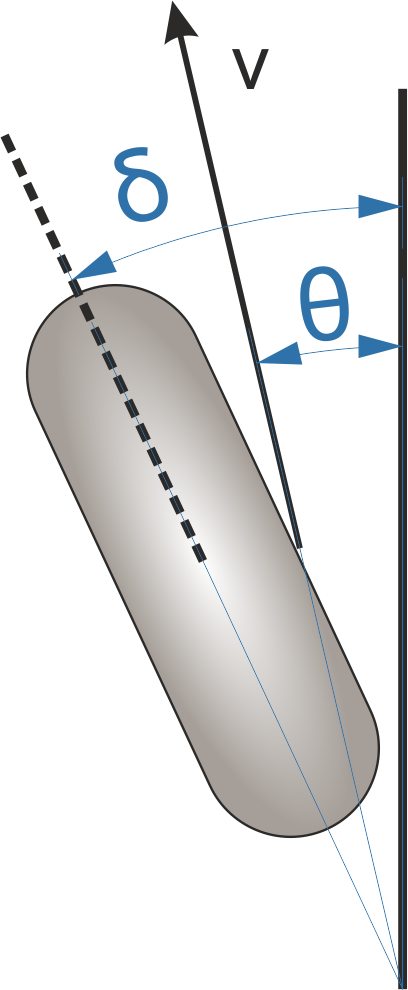
\includegraphics[width=70pt]{Abbildungen/slipAngle.png}
	\caption{Schräglaufwinkel}
	\label{fig:linLat}
\end{figure}


Für kleine Schräglaufwinkel besteht ein linearer Zusammenhang aus lateraler Kraft und Winkel. 
\begin{eqnarray}
F_{yf} = C_\alpha \alpha_f \\
F_{yr} = C_\alpha \alpha_r
\end{eqnarray}

Am Schaubild \ref{fig:pacejka} lässt sich dieser Bereich zwischen -1.5° und 1.5° sehr gut erkennen. Für größere Schräglaufwinkel kann kein linearer Verlauf mehr angenommen werden und es muss eine genauere Approximation des Kräfte gewählt werden. Hierfür wird die sogenannte \textit{Magic Formula}  \cite{magicFormula} verwendet. Dabei handelt es sich um eine mathematische Gleichung die sehr gut Messkurven approximiert welche auf Testständen gemessen werden.
Es wurde 1993 von Pacejka und Bakker entwickelt und eignet sich sowohl für die Berechnung der longitudinalen wie auch der lateralen Kräfte. Bei Eingabe des Schräglaufwinkels in \(x\) erhält man die lateral auf die Straße wirkende Kraft \(F_y\). 
\begin{equation}
F_y = D\sin[C\arctan{Bx - E(Bx - \arctan(Bx))}]
\label{eq:magicF}
\end{equation}

Die Parameter, welche für die \textit{Magic Formula} benötigt werden, wurden vom High Octane Motorsports e.V. zur Verfügung gestellt.

\begin{table}[]
	\centering
	\begin{tabular}{l|l}
		\hline
		Parameter	& Wert \\ \hline
		\(B\)	&  0.71 \\
		\(C\)	&  1.41 \\
		\(D\)	&  1.00 \\
		\(E\)	& -0.20 \\

	\end{tabular}
	\caption{Magic Formula Parameter}
	\label{tireParam}
\end{table}

\begin{figure}[ht!]
	\centering
	\begin{tikzpicture}
\begin{axis}[
width = 0.8\textwidth,
height = 0.5\textwidth,
xlabel=Schräglaufwinkel in rad,
ylabel=Laterale Seitenkraft in kN,
legend pos=north west]

\addplot [color=blue, line width=0.5mm] table [x index=0, y index=1]{Data/tireModel.dat};
\addplot [color=green,line width=0.5mm] table [x index=0, y index=2]{Data/tireModel.dat};

\addlegendentry{lin. Reifenmodell};
\addlegendentry{nichtlin. Reifenmodell};


\end{axis}
\end{tikzpicture} 
	\caption{Reifenmodell}
	\label{fig:pacejka}
\end{figure}

Ähnlich wie bei \(F_y\) wird auch die Kraft welche das Fahrzeug in Längsrichtung beschleunigt \(F_x\) durch den Schlupf berechnet. Dieser hängt direkt von der Geschwindigkeit und Raddrehzahl ab. 
Da für die Bestimmung dieser jedoch eine Motorsimulation vonnöten wäre, wird \(F_x\) direkt aus der Motorleistung, Reibung und Luftwiderstand berechnet (siehe Abschnitt \ref{dynModel}) und durch \(F_{max}\) begrenzt. \(F_{max}\) entspricht der maximalen Kraft, die der Reifen übertragen kann.\\
\begin{equation}
F_x <= F_{max}
\end{equation}
Der Zusammenhang zwischen lateraler und longitudinaler Kraft wird über den \textit{Kammschen Kreis} modelliert (siehe Schaubild \ref{fig:kamKreis}). Dieser schränkt die wirkenden Kräfte so ein, dass die Hypotenuse aus \(F_x\) und \(F_y\) sich maximal auf einem Einheitskreis bewegen kann. Der Radius entspricht maximalen Kraft welche die Reifen übertragen können (\(F_{max}\)).

\begin{eqnarray}
F <= F_{max} \\
F_{ll} = \sqrt{F_x^2 + F_y^2}  \\
\end{eqnarray}
Falls die Kraft $F_{ll}$ größer als $F_{max}$ ist, wird das Verhältnis der Kräfte berechnet und auf $F_{max}$ herunterskaliert.

\begin{eqnarray}
\alpha = \arctan(F_x, F_y)\\
F_x = F_{max} \sin(\alpha)\\
F_y = F_{max} \cos(\alpha)\\ 
\end{eqnarray}

\begin{figure}[ht!]
	\centering
	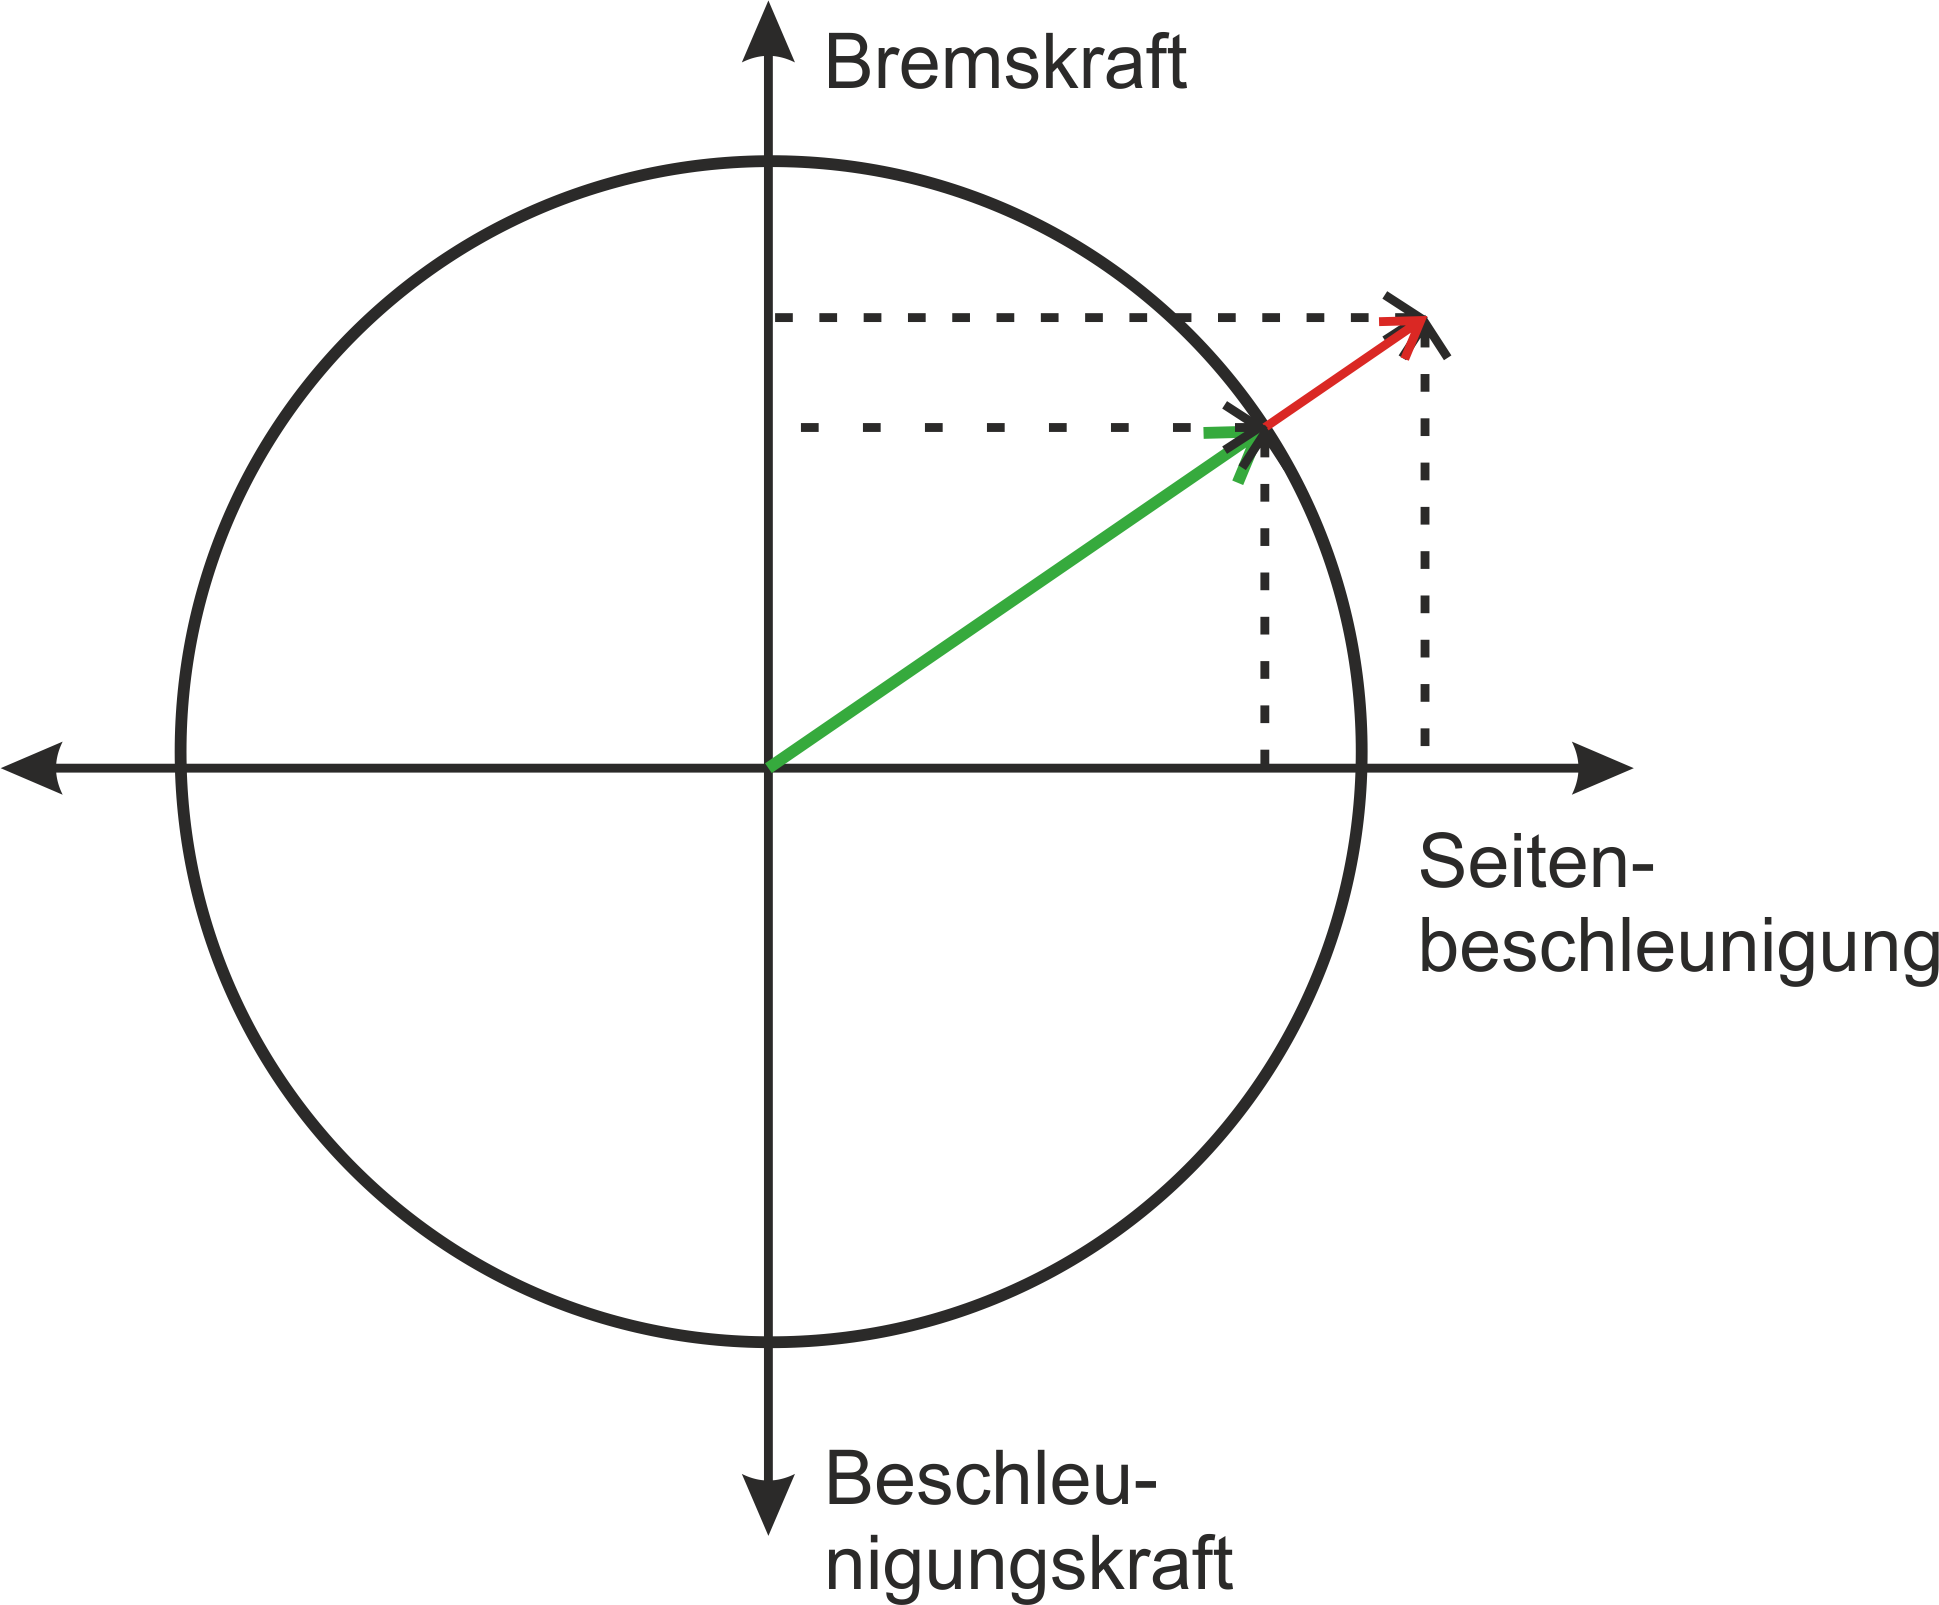
\includegraphics[width=250pt]{Abbildungen/kamKreis.png}
	\caption{Kammscher Kreis: Zusammenhang von longitudinaler, lateraler und maximaler Reifenkraft}
	\label{fig:kamKreis}
\end{figure}

Der aufmerksame Leser wird bemerkt haben, dass bei einem gleichen Anteil an longitudinaler und lateraler Kraft die Reifen das größte Moment auf die Straße übertragen können. Dieser Punkt wird von Rennfahrern versucht in Kurven zu treffen, um das gesamte Potenzial der Reifen auszunutzen.


Mit dem Wissen wie die longitudinalen und lateralen Kräfte berechnet werden, kann nun ein genaueres Systemmodell genutzt werden.

\subsection{Dynamisches Fahrzeugmodell}
\label{dynModel}

Die Basis ist, wie auch schon beim kinematischen Modell, das \textit{bicycle model}. Es wird nun um die durch das zweite newtonsche Gesetz entstehenden Kräfte entlang der \(y\)-Achse erweitert.

\begin{equation}
ma_y = F_{yf} + F_{yr}
\end{equation}   


Wobei \(a_y\) aus zwei Anteilen besteht, der Querbeschleunigung \(\ddot{y}\) und der Zentripetalkraft \(\dot{x} \dot{\psi}\).  
Die Kräfte \(F_{yf}\) und \(F_{yr}\) greifen jeweils am vorderen \((.)_f\) und hinteren \((.)_r\) Rad (siehe Schaubild \ref{fig:dynModel}). 

\begin{figure}[hb!]
	\centering
	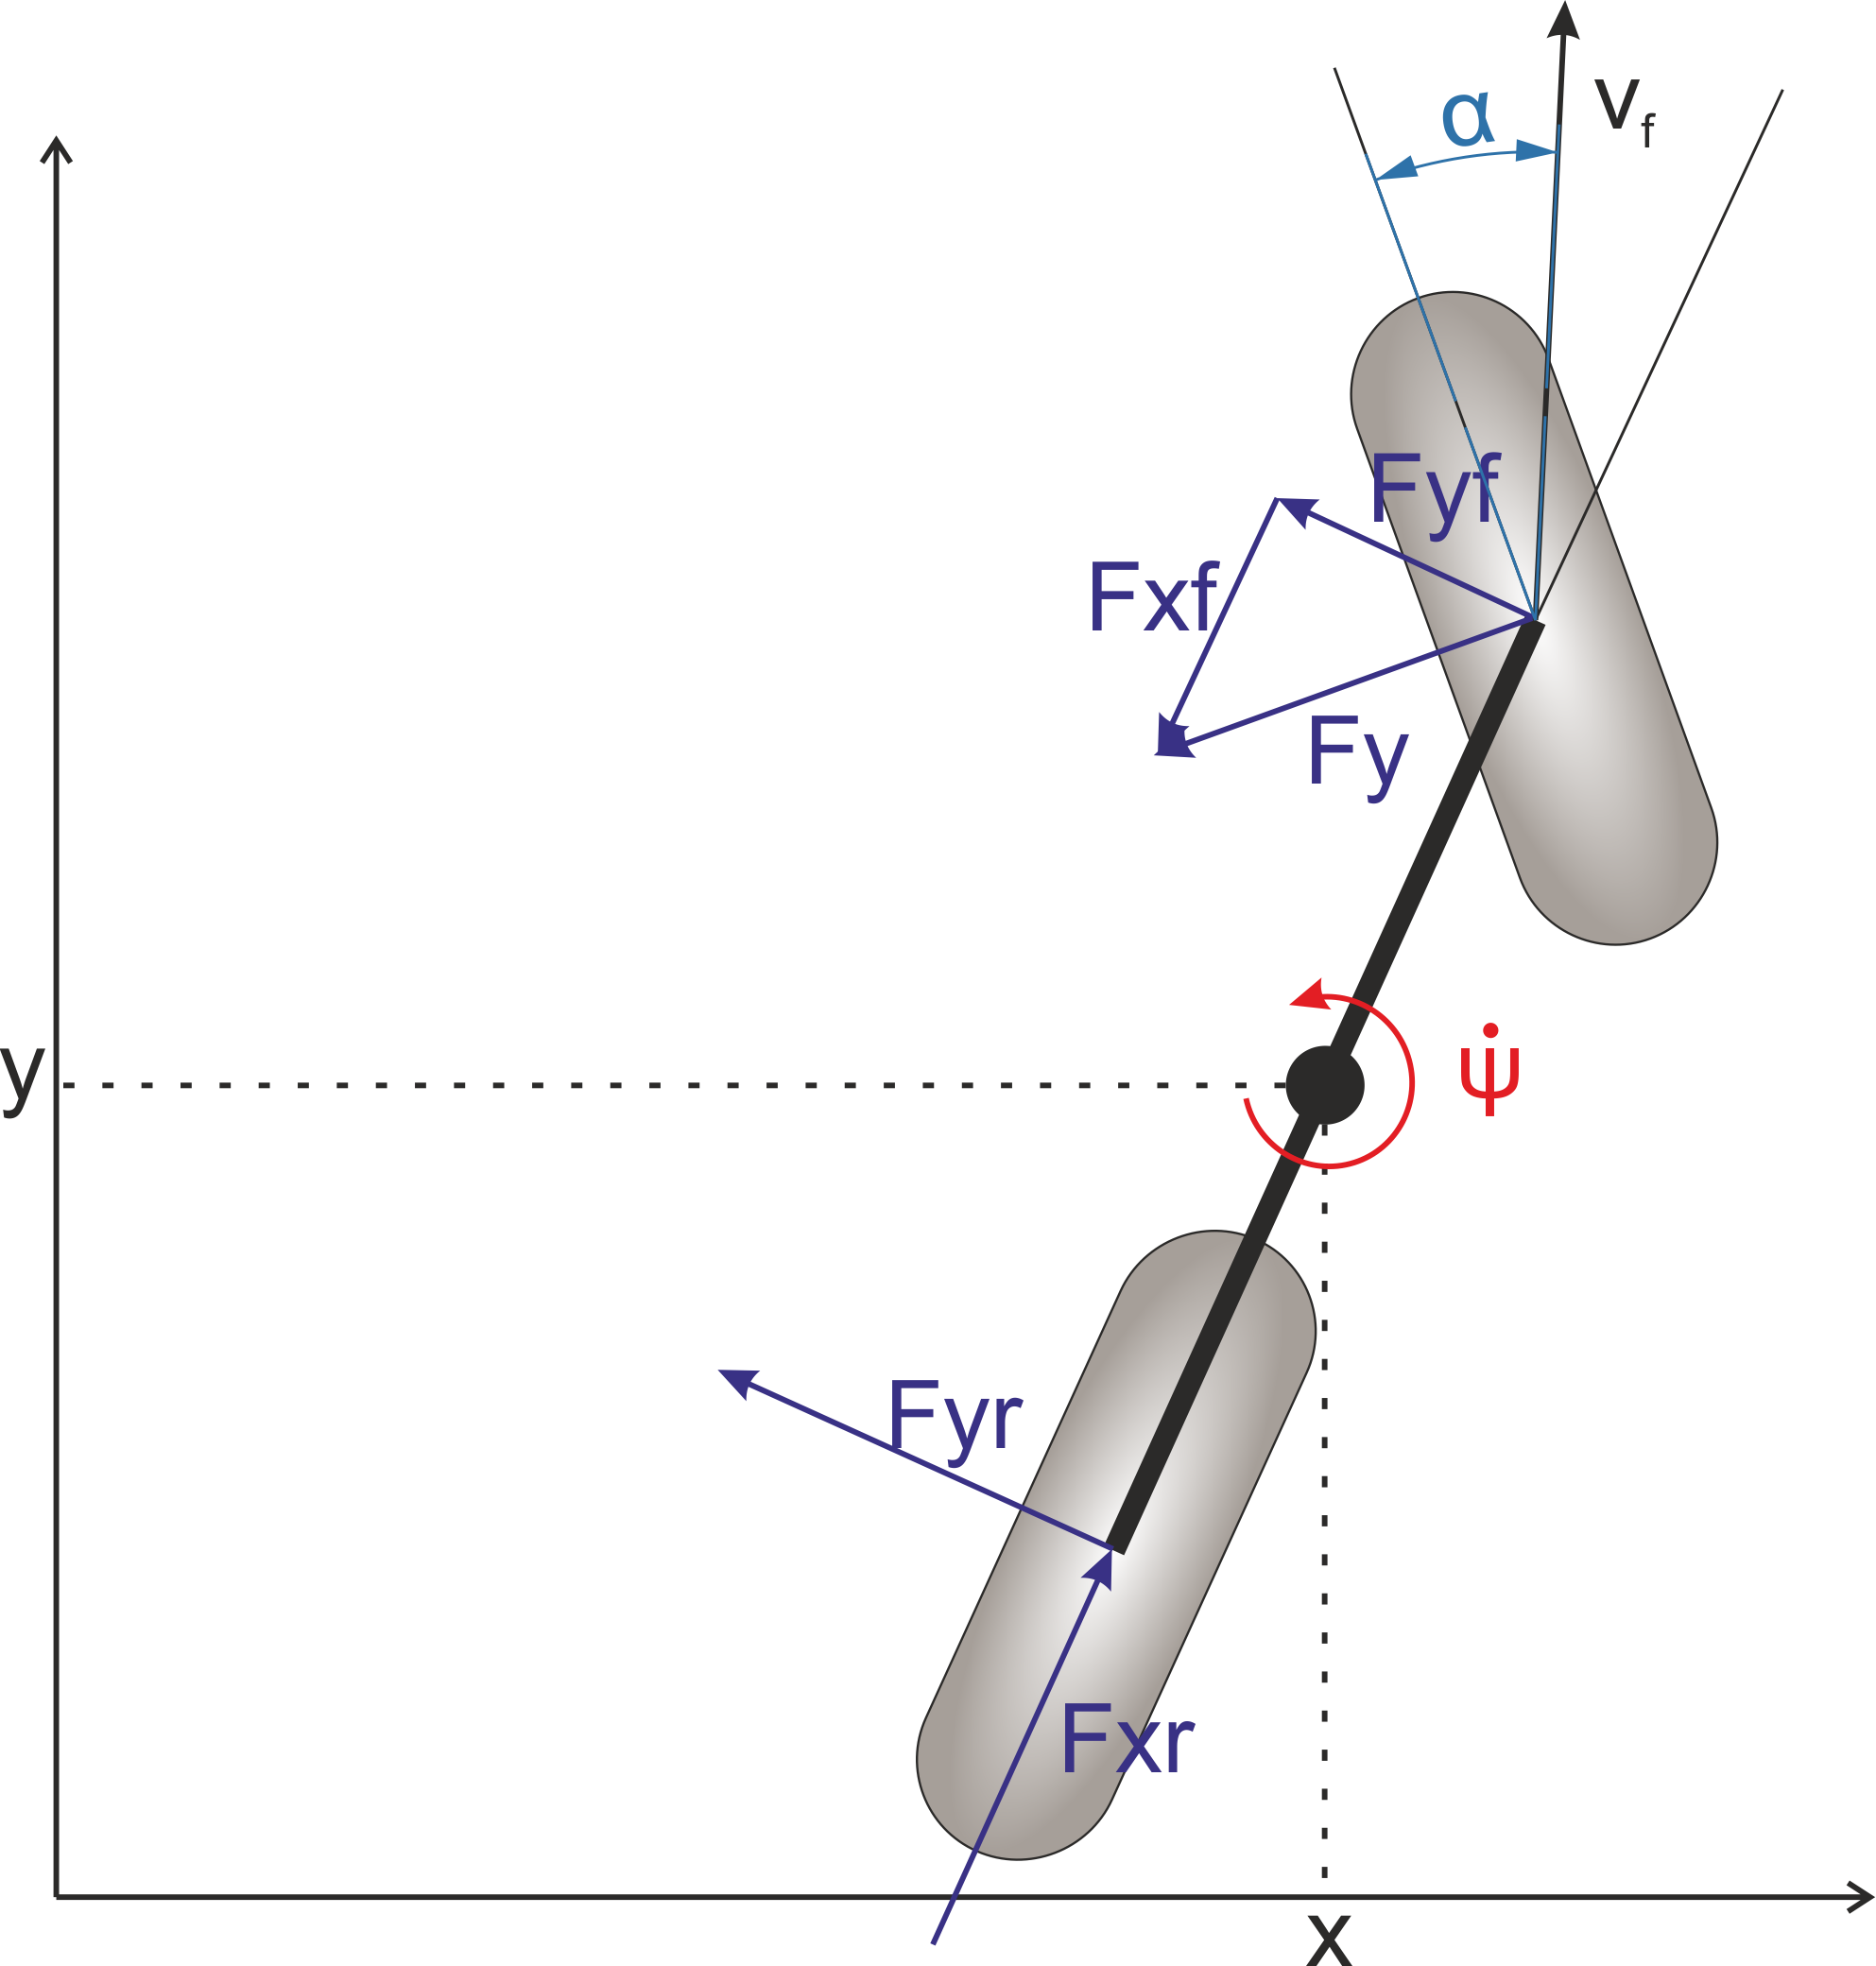
\includegraphics[width=300pt]{Abbildungen/dynBicycle.png}
	\caption{Dynamic Vehicle Model}
	\label{fig:dynModel}
\end{figure}




Unter Einbezug des Trägheitsmoments \(I_z\) des Fahrzeugs, kann das Drehmoment um die \(z\)-Achse betrachtet werden.
\begin{equation}
I_z \ddot{\psi} = l_f F_{yf} - l_r F_{yr}
\end{equation}

Als Ergebnis lassen sich die Gleichungen für Longitudinal-, Lateral- und Drehbewegung aufstellen.

\begin{eqnarray}
m \ddot{x} = m \dot{y} \dot{\psi} + F_x \\
m \ddot{y} = - m \dot{x} \dot{\psi} + F_y \\
I \ddot{(\psi)} = l_f F_{yf} - l_r F_{yr}
\end{eqnarray}

Die Kräfte \(F_{x}\) und \(F_{y}\) wirken auf den Schwerpunkt des Fahrzeugs und setzen sich aus den Einzelkomponenten der Radkräfte zusammen.

\begin{eqnarray}
F_x = F_{xf} + F_{xr} \\
F_y = F_{yf} + F_{yr}
\end{eqnarray}

Diese hängen ab von den lateralen \((.)_C\) und longitudinalen \((.)_l\)    Radkräften und dem Lenkwinkel. Da das Vorderrad nicht angetrieben wird, besitzt es keinen longitudinalen Anteil. 

\begin{eqnarray}
F_{xf} =& - 2 F_{Cf} \sin(\delta_f) \\
F_{yf} =& 2 F_{Cf} \cos(\delta_f) \\
F_{xr} =&   F_{lr} \\
F_{yr} =& 2 F_{Cr}
\end{eqnarray}
Es ist zu beachten, dass das Fahrzeug in der Realität vier Reifen besitzt und daher die Kräfte mit zwei multipliziert werden müssen.


Die Kräfte \(F_{Cf}\) und \(F_{Cr}\) werden durch die \textit{magic formula} wie im letzten Abschnitt \ref{tireModel} berechnet.
Die dafür benötigten Schräglaufwinkel werden durch folgende Formeln bestimmt:

\begin{eqnarray}
\alpha_f = \delta_f - \arctan(\frac{\dot{y} + l_f \dot{\psi}}{\dot{x}}) \\
\alpha_r = - \arctan(\frac{\dot{y} - l_r \dot{\psi}}{\dot{x}})
\end{eqnarray}

\subsection*{Longitudinale Kräfte}
Da keine Simulation des Motors genutzt wird, müssen die Kräfte \(F_{lr}\) welche die Reifen longitudinal auf die Straße bringen anders als über den Schlupf berechnet werden.
Dies wird realisiert über die maximale Motorleistung und \(F_{max}\).

\begin{eqnarray}
F_{lr_{acc}} = \frac{P_{engine} * throttle }{|\dot{x}|} \label{long_dyn_engine}\\
F_{lr_{acc}} <= 2 F_{max} \label{long_dyn_max}\\
F_{lr_{dec}} = - 2 F_{max} * break\\
\end{eqnarray}
Die Berechnung der Reifenkräfte ist für Beschleunigung und Bremsvorgang unterschiedlich.

Beschleunigt das Fahrzeug, wirkt nicht nur die Rollreibung der longitudinalen Kraft des Motors entgegen, sondern auch der Luftwiderstand. Es wird von einem Rennkurs ausgegangen der keine Steigung besitzt.
\begin{eqnarray}
F_{reib} = m \mu g \\
F_{aero} = \frac{1}{2} \rho C_d A_f \dot{x}^2
\end{eqnarray}

Die resultierende longitudinale Kraft (getrennt nach Beschleunigung und Bremsvorgang)
\begin{eqnarray}
F_lr = F_{lr_{acc}} - F_{reib} - F_{aero}\\
F_lr = F_{lr_{dec}} - F_{reib} - F_{aero}\\
\end{eqnarray}

wird mit den lateralen Kraft im Kammschen-Kreis verrechnet und in der finalen Bewegungsgleichung verwendet.

\begin{eqnarray}
\dot{X} =& \dot{x} \cos(\psi) - \dot{y} \sin(\psi) \\
\dot{Y} =& \dot{x} \sin(\psi) - \dot{y} \cos(\psi) \\
m \ddot{x} =& m \dot{y} \dot{\psi} + F_{xf} +  F_{xr}\\
m \ddot{y} =& - m \dot{x} \dot{\psi} +  F_{yf} +  F_{yr} \\
I \ddot{\psi} =&  l_f F_{yf} -  l_r F_{yr} \\
\end{eqnarray}

Das Gleichungssystem kann auch in diskreter Form aufgestellt werden.

\begin{eqnarray}
X_{k+1} =& X_k + \Delta t(\dot{x}_k \cos(\Psi_k) - \dot{y}_k \sin(\Psi_k) \\
Y_{k+1} =& Y_{k} + \Delta t(\dot{x}_k \sin(\Psi_k) - \dot{y}_k \cos(\Psi_k) \\
\Psi_{k+1} =& \Psi_k + \Delta t \dot{\psi}_k \\
\dot{x}_{k+1} =&  \dot{x}_k + \Delta t (\frac{F_{xf_k} +  F_{xr_k}- F_a}{m} + \dot{y}_k \dot{\psi}_k) \\
\dot{y}_{k+1} =&  \dot{y}_k + \Delta t (\frac{ F_{yf_k} +  F_{yr_k}}{m} - \dot{x}_k \dot{\psi}_k)  \\
\dot{\psi}_{k+1} =& \dot{\psi}_k + \Delta t \frac{ l_f F_{yf} -  l_r F_{yr}}{I} \\
\end{eqnarray}

Im dynamische Fahrzeugmodell ändert sich damit auch der Zustandsvektor: \\
\(X\), \(Y\), \(x_d\), \(y_d\), \(\Psi\), \(\dot{\psi}\) \\
Der Steuervektor bleibt gleich.

Die zur Berechnung verwendeten Fahrzeugparameter wurden für das zum Verfassen dieser Arbeit aktuellstem Fahrzeug erfasst. Die Informationen hierfür sind aus dem CAD-Modell oder im Feld erfassten Testdaten entnommen worden (siehe Anhang).


\begin{table}[]
	\centering
	\begin{tabular}{l|l|l}
		\hline
		Formelzeichen	& Wert & Einheit \\ \hline
		\(l_f\)	&	1.09 & m\\
		\(l_r\)	&	0.9 & m\\
		\(l_b\)	&	1.99 & m \\
		\(r\)	&	0.2 & m \\
		\(m\)	&  	163 & kg\\
		\(I\)	&  	1000 & kgm\textsuperscript{2}\\
		\(A_f\)	&  	1.5 & m\textsuperscript{2}\\
		\(P_{engine}\) &  40,5 & kW\\
		\(C_d\)	&  	1.5 & - \\
		\(\rho\)	&  	1.225 & kg / m\textsuperscript{3}\\
		\(F_{max}\)	&  	3 & kN \\ 
	\end{tabular}
	\caption{Vehicle Parameter}
	\label{vehicleParam}
\end{table}





\section{Programmiersprachen}
\subsection{Python}

Zu Beginn der Arbeit wurde zuerst die Programmiersprache Python verwendet um den \ac{MPC}-Ansatz zu programmieren. Als Optimierer wurde ein \emph{\ac{SLSQP}}-Algorithmus verwendet. Dieser ist direkt in die SciPy-Bibliothek integriert und unterstützt Eingangs-, Ausgangs- und Zustandsbeschränkungen, ohne die es nicht möglich ist den \ac{MPC}-Algorithmus für die Fahrzeugregelung auszulegen. So lange die Anzahl der Prädiktionsschritte klein bleibt und 10 nicht überschreitet ist die Ausführungszeit gering genug um eine Aktualisierungsrate von 20 Hz zu erreichen. 

\begin{figure}[ht!]
	\centering
	
\begin{tikzpicture}
\begin{axis}[
width = 0.8\textwidth,
ylabel=Ausführungszeit in s,
xlabel=Prädiktionsschritte (N)]

\addplot [color=red, mark=x, line width=0.5mm] table [x index=0, y index=1]{Data/pythonBench.dat};
\end{axis}
\end{tikzpicture} 
	\caption{Ausführungszeiten für verschiedene  große Horizontlängen}
	\label{fig:pythonBench}
\end{figure}

Bei größeren Prädiktionsvektoren fällt die Geschwindigkeit jedoch sehr schnell ab. Der Benchmark \ref{fig:pythonBench} ist für das fertige Optimierungsproblem gemessen worden.
Dies liegt daran, dass der SLSQ- Algorithmus nicht für nichtlineare Probleme ausgelegt ist. Bessere Skalierung erhält man bei der Verwendung eines \textit{Solvers} der das Innere-Punkte-Verfahren nutzt. Dieser Algorithmus setzt jedoch, um gute Performance zu erreichen, wie in Abschnitt \ref{ipm} beleuchtet, die Kenntnis über die Ableitung der Systemfunktion voraus. Diese kann mit Frameworks wie: CasADi, PyADOL-C, PyCppAD berechnet werden \cite{DBLP:journals/corr/TurkinT16}. 
Eine Implementierung des \ac{MPC}-Ansatzes in CasADi wurde  aufgrund der schlechten Dokumentation abgebrochen und nach einer Alternativlösung gesucht. Das Ergebnis dieser Suche führte zur Verwendung einer neuen Programmiersprache. 


\subsection{Julia}
\label{julia}
Julia ist die Programmiersprache, die die Umsetzung des \acl{MPC}-Algorithmus effizient und performant ermöglichte. Sie wurde im Jahr 2009 von Jeff Bezanson, Stefan Karpinski, Viral B. Shah, and Alan Edelman ersonnen und ist damit noch eine sehr junge Sprache. Sie ist vor allem für numerische Analyse und wissenschaftliche Berechnungen entworfen worden und bietet in diesen Bereichen viele Funktionalitäten. Ebenfalls ein wichtiges Ziel bei der Entwicklung war es, ohne vorheriges Kompilieren sehr schnell zu sein und trotzdem weiterhin das \textit{general-purpose} Paradigma zu erfüllen. Ein Vergleich der Berechnungsgeschwindigkeit verschiedener Sprachen bezüglich viel genutzter Funktionen im wissenschaftlichen Umfeld ist in dem Benchmark \ref{fig:juliaBench} zu sehen.

\begin{figure}[ht!]
	\centering
	
\begin{tikzpicture}
\begin{axis}[
width = 1.0\textwidth,
height = 0.6\textwidth,
ymin=-1e0, ymax=1e1,
ylabel=Ausführungszeiten relativ zu C,
x tick label style={font=\small,text width=1.2cm,align=center},
xticklabels={Benchmark,C,Julia,LuaJIT,Go,Fortran,Java,Java-script,Matlab,Mathe-matica, Python},
legend pos=north west]

\addplot [color=red, only marks] table [x index=0, y index=1]{Data/juliaBench.dat};
\addplot [color=blue, only marks] table [x index=0, y index=2]{Data/juliaBench.dat};
\addplot [color=green, only marks] table [x index=0, y index=3]{Data/juliaBench.dat};
\addplot [color=black, only marks] table [x index=0, y index=4]{Data/juliaBench.dat};
\addplot [color=orange, only marks] table [x index=0, y index=5]{Data/juliaBench.dat};
\addplot [color=yellow, only marks] table [x index=0, y index=6]{Data/juliaBench.dat};
\addplot [color=purple, only marks] table [x index=0, y index=7]{Data/juliaBench.dat};
\addplot [color=brown, only marks] table [x index=0, y index=8]{Data/juliaBench.dat};
\addlegendentry{iteration pi sum}
\addlegendentry{recursion fibonacci}
\addlegendentry{recursion quicksort}
\addlegendentry{parse integers}
\addlegendentry{print to file}
\addlegendentry{matrix statistics}
\addlegendentry{matrix multiply}
\addlegendentry{mandelbrot}
\end{axis}
\end{tikzpicture} 
	\caption{Ausführungszeiten für verschiedene Sprachen}
	\label{fig:juliaBench}
\end{figure}

Die wichtigsten Feautres von Julia sind:
\begin{itemize}

	\item multiple dispatch \\Wird genutzt um die gleiche Methode für verschiedene Kombinationen an Eingabeparametern oder Variablentypen zu überladen. Bei dem Funktionsaufruf wird die am besten passende Methodendefinition aufgerufen. \\
	\item type inference \\Das automatische detektieren des Datentyps. Dies befreit den Programmierer vom festlegen des Typs und ermöglicht trotzdem Typprüfung. \\
	\item \ac{JIT} Kompilierung\\ Ein System, in dem ein \ac{JIT} Kompilierer implementiert ist, wandelt den Computer Code erst zur Laufzeit in Bytecode um. Der große Vorteil ist, dass während der Ausführung kontinuierlich Analysen durchgeführt werden, um Bereiche ausfindig zu machen die durch ein Neukompilieren eine signifikante Verbesserung bei der Ausführungszeit erfahren würden. \\
\end{itemize}

Obwohl es möglich wäre die einzelnen Bestandteile, welche nötig sind um den Model Predictice Control - Algorithmus zu berechnen, in Julia zu implementieren gibt es eine umfangreiche Erweiterung welche eine passende Schnittstelle für solche Probleme zur Verfügung stellt.

\subsubsection*{Jump}
Jump ist eine Erweiterung für Julia mit der sich mathematische Probleme modellieren und lösen kann. Es besitzt Schnittstellen für mehrere sowohl frei verfügbare, wie auch kommerzielle Optimierer, mit denen sich zum Beispiel lineare oder nichtlineare Probleme lösen lassen. Der große Vorteil von Jump ist, dass die Definition des mathematischen Problems unabhängig von dem verwendeten Optimierer ist und dieser damit leicht ausgetauscht werden kann (siehe Schaubild \ref{fig:jumpDiagram}). Ebenfalls ersichtlich ist das Jump sich direkt um die automatische Ableitung kümmert und so dem Programmierer sehr viel Arbeit erspart. 

\begin{figure}[ht!]
	\centering
	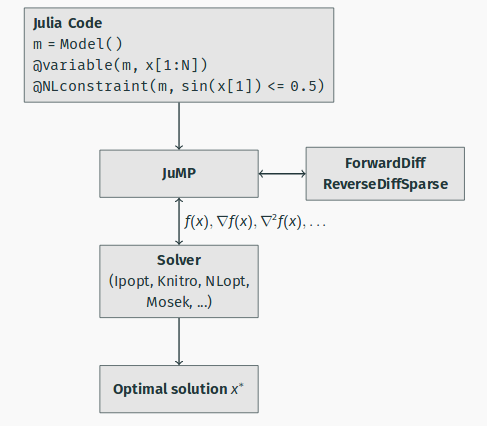
\includegraphics[width=150pt]{Abbildungen/jumpDiagram.png}
	\caption{Blockdiagramm von Jump}
	\label{fig:jumpDiagram}
\end{figure}

Die Syntax welche Jump für die Definition der Probleme vorsieht ähnelt der standardmäßigen mathematischen Definition, was die Anwendung intuitiv gestaltet. Zudem ist die Dokumentation sehr ausführlich.


\chapter{MPC zur Trajektionsplanung und Regelung}

Ein schneller Rennfahrer zeichnet sich dadurch aus, dass er genau abschätzen kann wie viel Kräfte die Reifen des Fahrzeugs auf die Straße übertragen können. Die Kunst liegt also darin, möglichst in jeder Fahrsituation das gesamte Potential voll auszunutzen. Außerdem kann er sich dynamisch an Änderungen der Streckeverhältnisse anpassen und versucht immer die Idealtrajektorie zu treffen. Die Definition dieser ist, möglichst viel Streckenlänge in der kleinstmöglichen Zeit zurückzulegen. Für eine Gerade oder eine einzige Kurve ist dies, wie in Abbildung \ref{fig:idealTrajektorie} dargestellt, leicht zu berechnen. Der so genannte Scheitelpunkt markiert hierbei den Punkt des geringste Radius und der kleinsten Geschwindigkeit. An diesem Punkt muss das Fahrzeug im besten Fall genau die Seitenbegrenzung tangieren. 
Bei komplexeren Streckengefügen kann es jedoch von Vorteil sein, eine Kurve eventuell nicht ideal auszufahren um im späteren Verlauf einen größeren Geschwindigkeitsgewinn in einer anderen Kurve einfahren zu können.

\begin{figure}[ht!]
	\centering
	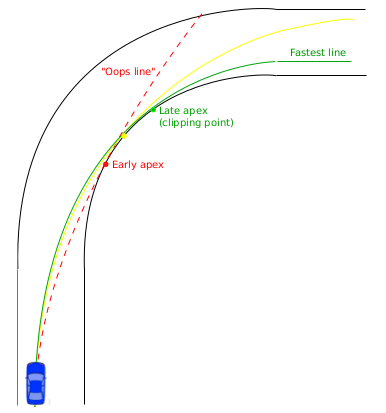
\includegraphics[width=150pt]{Abbildungen/idealTrajektorie.png}
	\caption{Ideale Trajektorie für eine 90 Grad Kurve (Dummy Bild)}
	\label{fig:idealTrajektorie}
\end{figure}


Um all dies mit dem \ac{MPC}-Algorithmus nachzustellen wird im Folgenden auf die einzelnen Schritte bei der Entwicklung eingegangen.

Zu Beginn hätte die Möglichkeit bestanden die Regelung der lateralen und longitudinalen Führung des Fahrzeuges zu trennen. 
Vorteile hierfür wären gewesen:
\begin{itemize}
	\item Einfachere Anpassung der Parameter für das reale Fahrzeug.
	\item Robustheit. Der Ausfall eines Reglers würde zumindest noch eine eingeschränkte Kontrolle ermöglichen.
	\item Zwei einfacher zu berechnende Probleme. Da die Berechnungszeit nicht linear mit der Komplexität steigt, wären hier möglicherweise deutliche Geschwindigkeitssteigerungen möglich.
	\item Ein weniger komplexer \ac{MPC}-Ansatz ist einfacher zu testen und entwickeln.
\end{itemize}

Die Vorteile werden aber mit dem Nachteil begleitet, dass bei einem Rennauto die longitudinale und laterale Bewegung des Fahrzeugs ganz signifikant miteinander verbunden ist. Durch die Trennung kann keine optimale Lösung mehr gefunden werden. 
Zudem ist die Integration komplexer, da beide Regler gleichzeitig laufen und ihre Berechnungen miteinander ausgetauscht werden müssen.
Aufgrund des Anwendungsszenarios wurde sich gegen den zweigeteilten Ansatz entschieden.


Der erste Schritt ist das Erstellen des Vektors an Einflussparametern $\vec{X}$. Er setzt sich immer aus der Kombination von Systemzustand und Steuerparametern zusammen  $\vec{x} = [x, y, v, \psi, a, \delta ]^T $ (siehe \ref{kinematicModel}). 
Dieser Teilvektor wird dann für die Anzahl der gewünschten Prädiktionsschritte \(N\) mal in $\vec{X}$ wiederholt. Da zusätzlich zu den Prädiktionsschritten auch der aktuelle Fahrzeugzustand benötigt wird, besteht der Vektor also aus $N+1$ Teilvektoren $\vec{x}$. In der Abbildung \ref{fig:predictionMpc} ist grafisch dargestellt, wie man sich die Prädiktion für $N=3$ vorstellen kann. Zwischen jedem der einzelnen Schritte wird ein $\Delta t$ angenommen, welches der Abtastrate der Positionsschätzung entspricht also $\frac{1}{20} s$. Obwohl immer nur der erste Steuerbefehl des berechneten Steuervektors im realen System angewandt wird, ist der Vektor trotzdem von nutzen. Sollte die Optimierung, unterbrochen durch andere Prozesse, einmal nicht schnell genug sein, können die Steuerbefehle aus der vorherigen Optimierung verwendet werden. Dies geht, solange die Zeitverzögerung kleiner als die gesamte Zukunftsprädiktion ist. Obwohl man diese Werte zum Regeln nutzen kann, nimmt aufgrund von Modellfehlern die Güte der berechneten Werte mit \(n\) ab. Man ist also bestrebt den Algorithmus mit der gleichen Rate wie die Positionsschätzung laufen zu lassen. 

  
\begin{figure}[ht!]
	\centering
	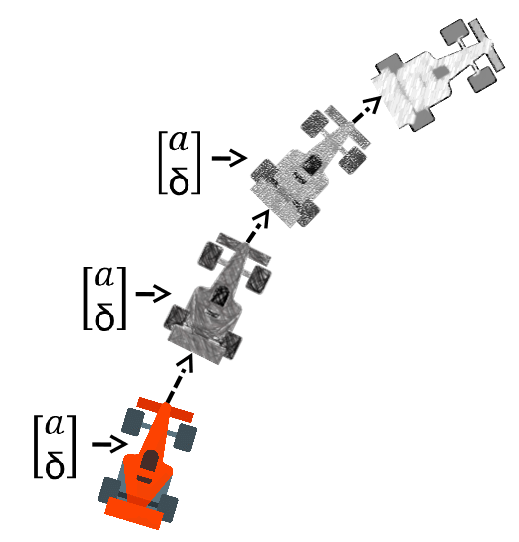
\includegraphics[width=150pt]{Abbildungen/prediction.png}
	\caption{Grafische Visualisierung der Prädiktion abhängig von den Steuerparametern für drei Schritte in die Zukunft}
	\label{fig:predictionMpc}
\end{figure}
Nachdem der Vektor mit den Einflussparametern definiert ist, werden im nächsten Schritt alle Beschränkungen sukzessive ergänzt.

\section{Fahrzeugmodell}
Zu Beginn haben die Teilvektoren $\vec{x}$ keinen Zusammenhang untereinander. Da jedoch die einzelnen Prädiktionsschritte voneinander über den Fahrzeugzustand, Steuerparameter und das Fahrzeugmodell zusammenhängen, werden im zweiten Schritt die Beschränkungen hierfür integriert. Dazu wird die diskretisierte Form des Systemmodells \ref{kinDiscrete} genutzt, um immer zwei aufeinander folgende Schritte miteinander zu verknüpfen. Die entstehenden Gleichheitsbedingungen sind im Anhang unter \ref aufgeführt.\\

Zusätzlich zu der Systembeschreibung fehlen noch Einschränkungen für den Optimierer, welche die physikalischen Eigenschaften des Rennautos abbilden.
Dazu zählen die maximale Geschwindigkeit, Beschleunigung und Lenkwinkel. 
Diese Beschränkungen werden auch für jeden der Teilvektoren hinterlegt. 
Zusammen mit dem Fahrzeugmodell benötigt das \ac{MPC} noch eine Kostenfunktion damit der Optimierer überhaupt einen Anlass hat das Rennauto zu beschleunigen.


\section{Kostenfunktionen}
\label{costFunctions}
Erst eine geeignete Kostenfunktion führt zu der Planung einer Trajektorie die das Rennauto um den Kurs führt. Es wurden zwei verschiedene Kostenfunktionen implementiert:

\subsubsection*{Maximalgeschwindigkeit}  
In dieser Funktion wird die Summe aller Geschwindigkeitswerte der einzelnen Prädiktionsschritte addiert und als Kosten versucht zu maximieren. \\
$f(\vec{X}) =  \sum_{1}^{N+1} v_i$ \\
Die Berechnung startet nicht beim $0$ten Schritt, da dieser dem aktuellen Zustand entspricht und der Optimierer keinen Einfluss mehr auf diesen hat. Die Idee hinter dieser Funktion ist, dass sie einfach zu berechnen ist und im Vorhersagehorizont eine möglichst schnelle Trajektorie entsteht.

\subsubsection*{Zielpunkt Distanzminimierung}
Für diese Kostenfunktion wird vor den letzten Prädiktionsschritt ein virtuelles Ziel definiert und die Distanz des $N+1$ Schrittes zu diesem Ziel minimiert. Der Optimierer wird also versuchen Steuerparameter zu finden die ihn möglichst schnell auf dieses Ziel zu fahren lassen. Das virtuelle Ziel wird nach jedem Update wieder so neu positioniert, dass das Rennauto den Punkt niemals erreichen kann und damit konstant schnell weiter fährt. Eine bildliche Darstellung der Kostenfunktion ist in Abbildung \ref{fig:costGoalDist} zu sehen. 

\begin{figure}[ht!]
	\centering
	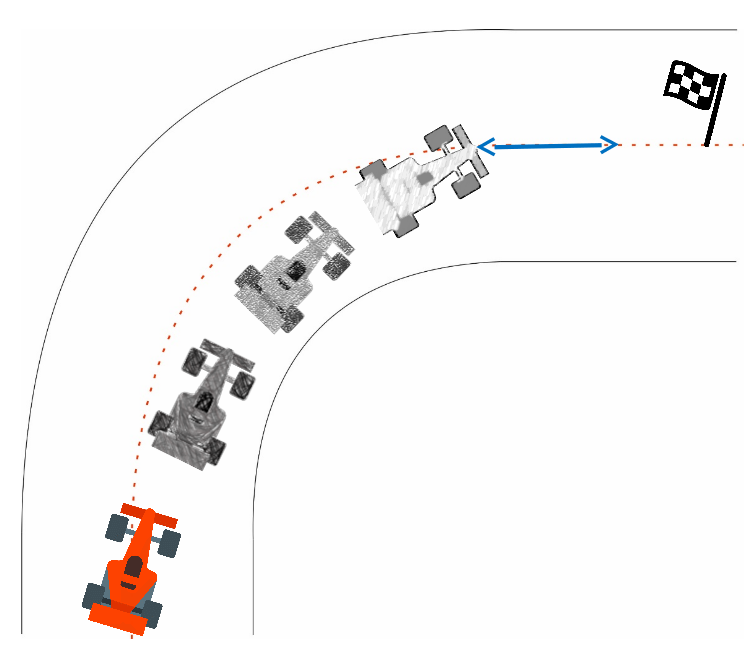
\includegraphics[width=200pt]{Abbildungen/cost_goal_dist.png}
	\caption{Zielpunkt Distanzminimierung: Das virtuelle Ziel wird immer weit genug vor dem Fahrzeug her geführt, so dass es nie erreicht werden kann.}
	\label{fig:costGoalDist}
\end{figure}

\subsubsection*{Maximieren der Streckendistanz}
Um eine Kostenfunktion zu finden welche einer Idealtrajektorie am nächsten kommt, muss überlegt werden wie man diese Messbar macht. Die bestmögliche Trajektorie ist diejenige welche für ein $\Delta t$ die zurückgelegte Strecke nicht bezogen auf das Fahrzeug sondern auf den Rennkurs maximiert. Dies lässt sich durch eine Umformung zu einer Minimierung der nach dem Zeitschritt übrig bleibenden Reststrecke umformen. Mit der Vereinfachung, dass das Ziel und damit die Reststrecke in einer Distanz vorm dem letzten Prädiktionsschritt sich befindet welchen das Fahrzeug nicht erreichen kann. Der Unterschied zur Kostenfunktion welche die Distanz minimiert ist, dass sich die Differenz nicht auf einen Punkt sondern auf eine Gerade senkrecht zur Rennkursmitte bezieht.
Realisiert wird dies durch eine \emph{vector rejection}
$d = |a - \frac{ab}{bb}b| $. Dies ist in der Abbildung \ref{fig:maxDist} bildlich veranschaulicht.

\begin{figure}[ht!]
	\centering
	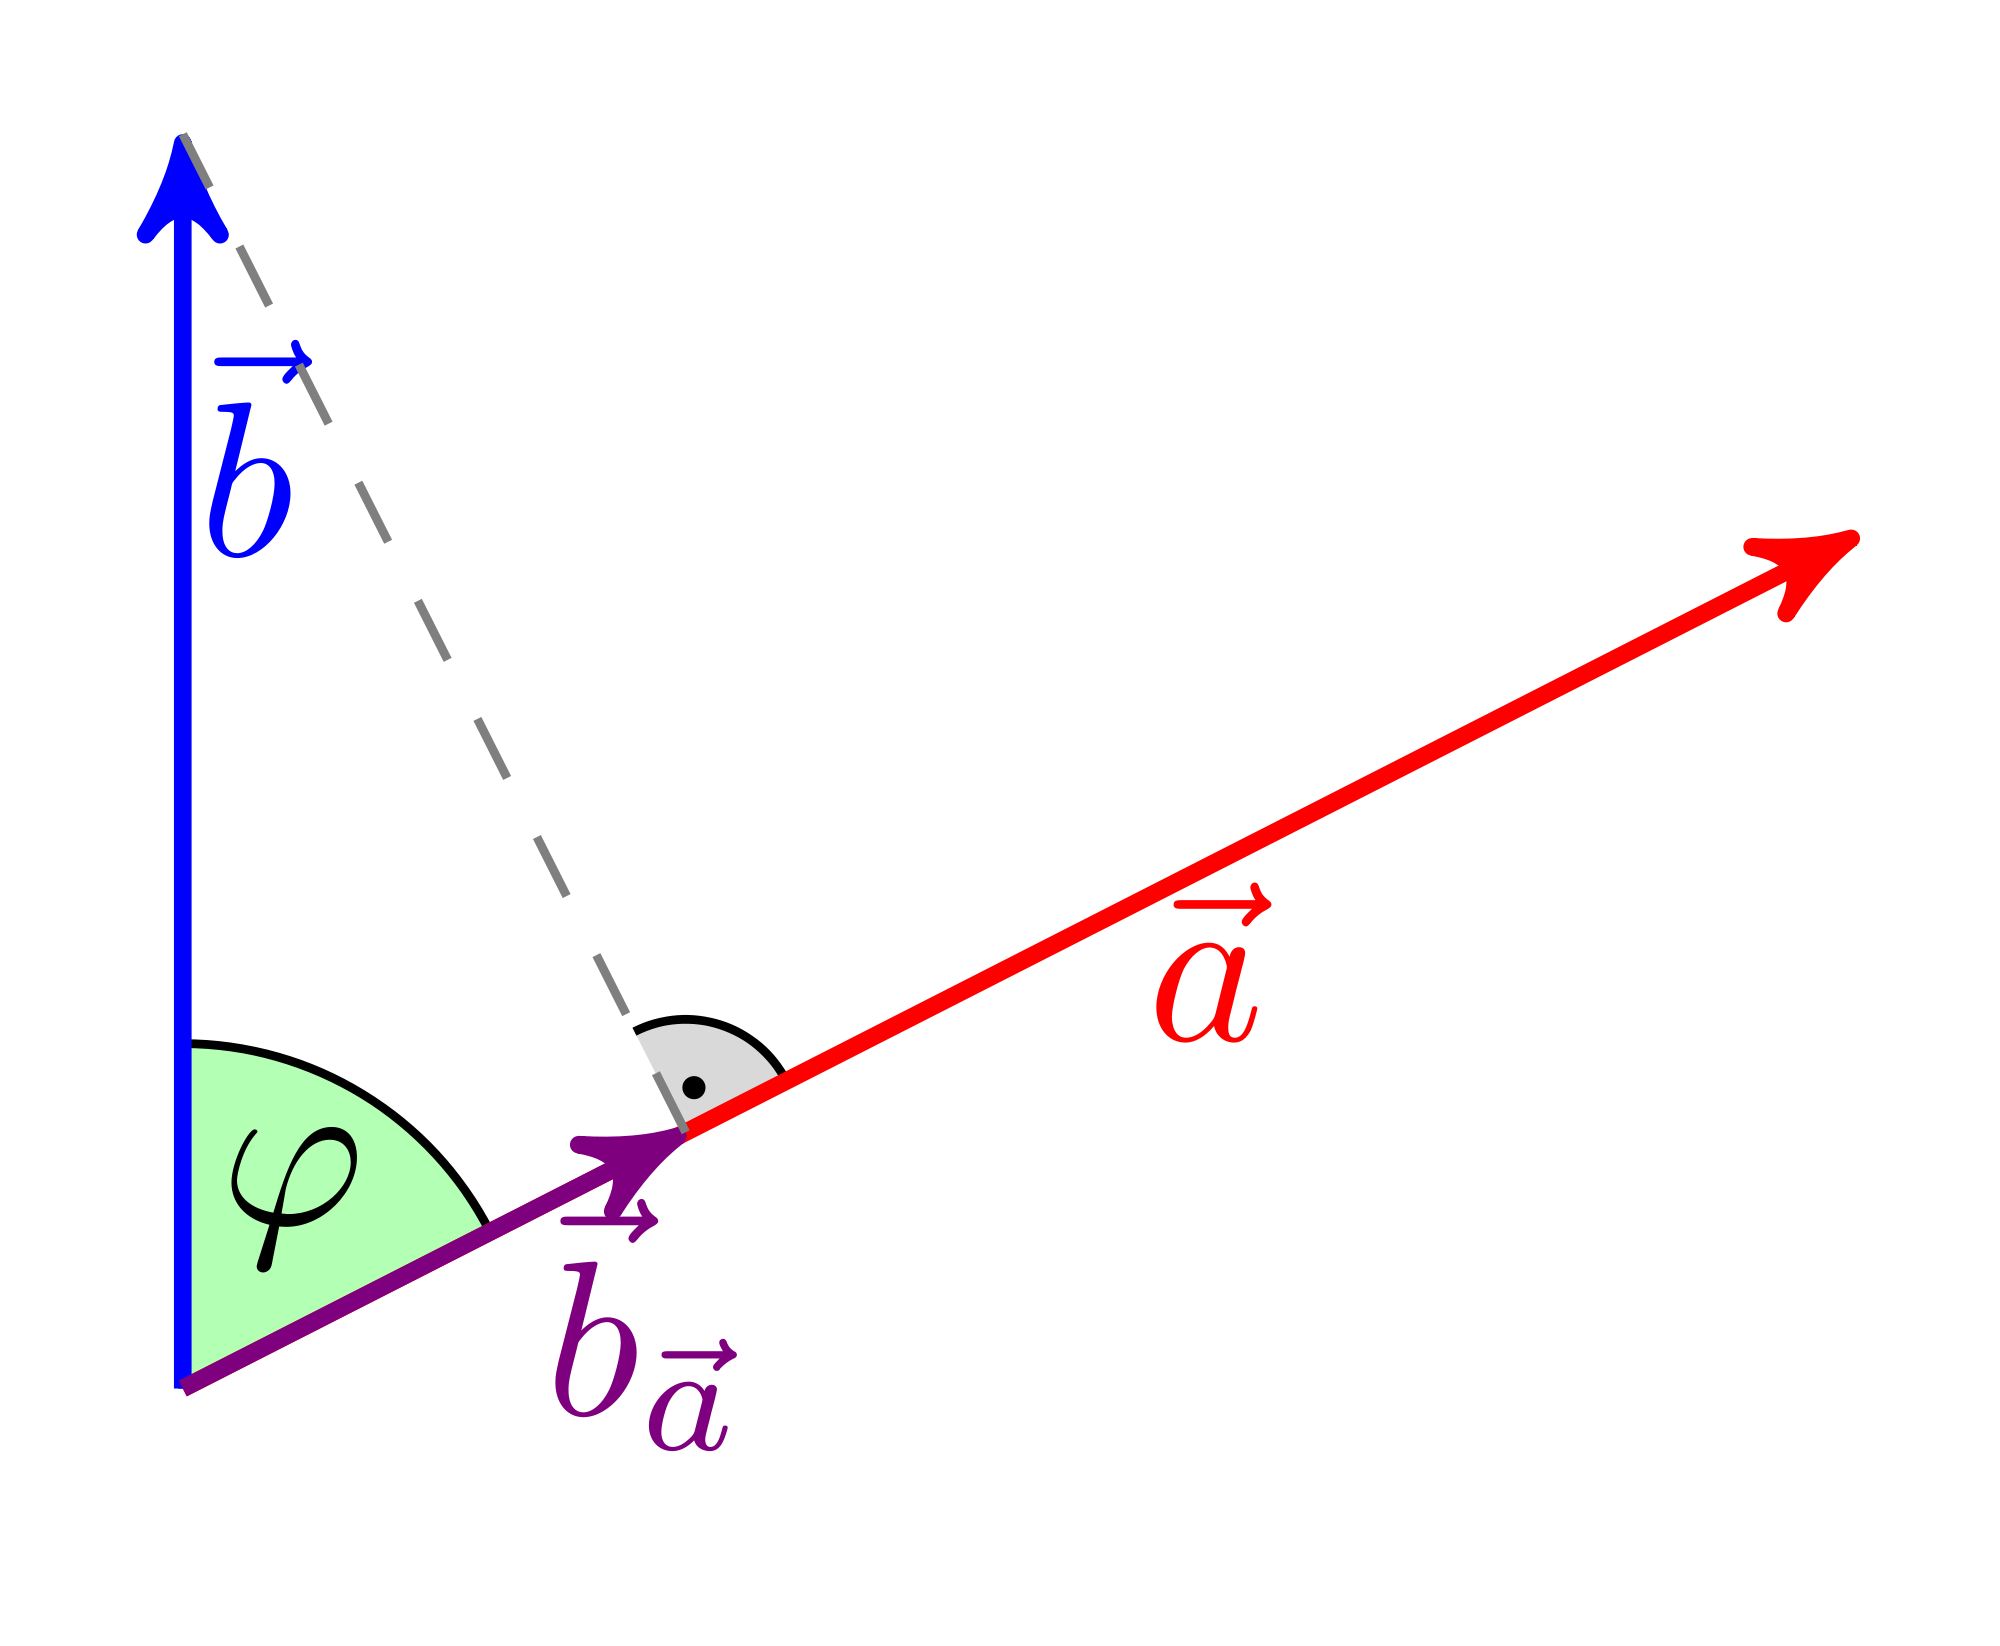
\includegraphics[width=200pt]{Abbildungen/maxDist.png}
	\caption{Maximieren der Streckendistanz (Dummy)}
	\label{fig:maxDist}
\end{figure}

\section{Strecken-, und Positionsbeschränkung}
\label{trackAndPosConstraint}
Die Kostenfunktionen führen dazu, dass der Optimierer die Steuerparameter so anpasst, dass die Kosten minimal werden. Dies würde auf einem Rennkurs zum Abkürzen bei Kurven führen, da in diesem Fall die Kosten geringer werden. Um dies zu verhindern wurde eine zusätzliche Streckenbeschränkung eingeführt. Diese basiert auf zwei Tangenten die für jedem Prädiktionsschritt an die Fahrbahn Außen-, und Innenseite projiziert werden. So lange sich das Rennauto innerhalb dieser Tangenten bewegt ist die Beschränkung erfüllt. Während des Optimierungsvorgangs wird die Position der Tangenten nicht verändert, sondern vor der Optimierung fix gesetzt. Um für den Prädiktionsschritt \(n\) den passenden Streckenabschnitt zu suchen, für den die Beschränkung ausgelegt wird, kann auf die Ergebnisse der vorausgehenden Optimierung zurückgegriffen werden. Die Position des $n+1$-Schritt wird gewählt und als Ausgangssituation gewählt. Für den letzten Schritt \(N\) ist dies nicht möglich, hier wird mithilfe der Geschwindigkeit und Orientierung ein virtueller Punkt projiziert.   

\begin{figure}[ht!]
	\centering
	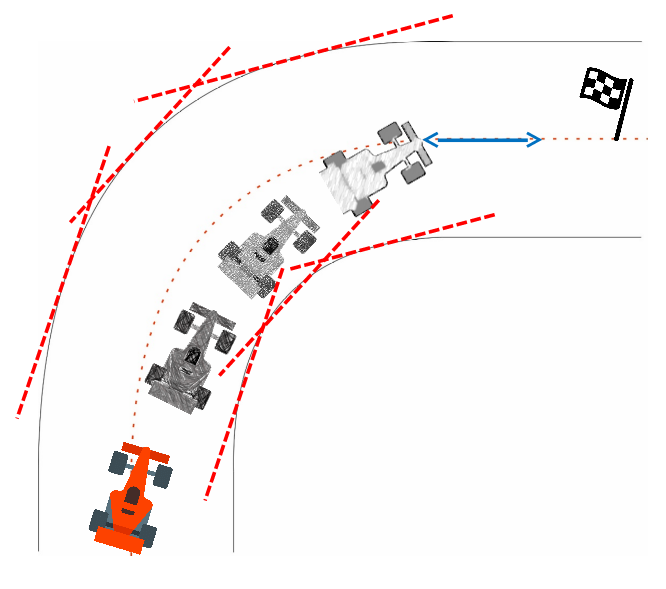
\includegraphics[width=200pt]{Abbildungen/tangentialConstraint.png}
	\caption{Tangentiale Begrenzung hält das Fahrzeug auf der Fahrspur}
	\label{fig:costGoalDist}
\end{figure}
Dieses Verfahren funktioniert nur, da die Beschleunigung des Rennautos physikalischen Grenzen unterliegt und sich daher immer in einem bestimmten Bereich um den Punkt herum bewegt, welcher bei gleichbleibender Geschwindigkeit $\Delta t * v$ Meter entfernt von seinem Vorgängerzustand liegt. Wenn sich dieser Punkt in einer Kurve direkt an der Streckenmarkierung befindet, könnte das Fahrzeug sich trotzdem, trotz erfüllen der Tangentialbeschränkung, vom Kurs herunter bewegen. Dies wird dadurch verhindert, dass der nächste Prädiktionsschritt in diesem Fall seine Beschränkung nicht mehr erfüllen würde.
Mathematisch lassen sich die Tangenten durch eine Vektorprojektion $d = \frac{a*b}{|b|}$ realisieren. Dabei a entspricht dem Vektor vom Mittelpunkt der Strecke zum Massenschwerpunkt des Rennautos und b dem Vektor vom Mittelpunkt zum Rand des Rennkurses. 

\begin{figure}[ht!]
	\centering
	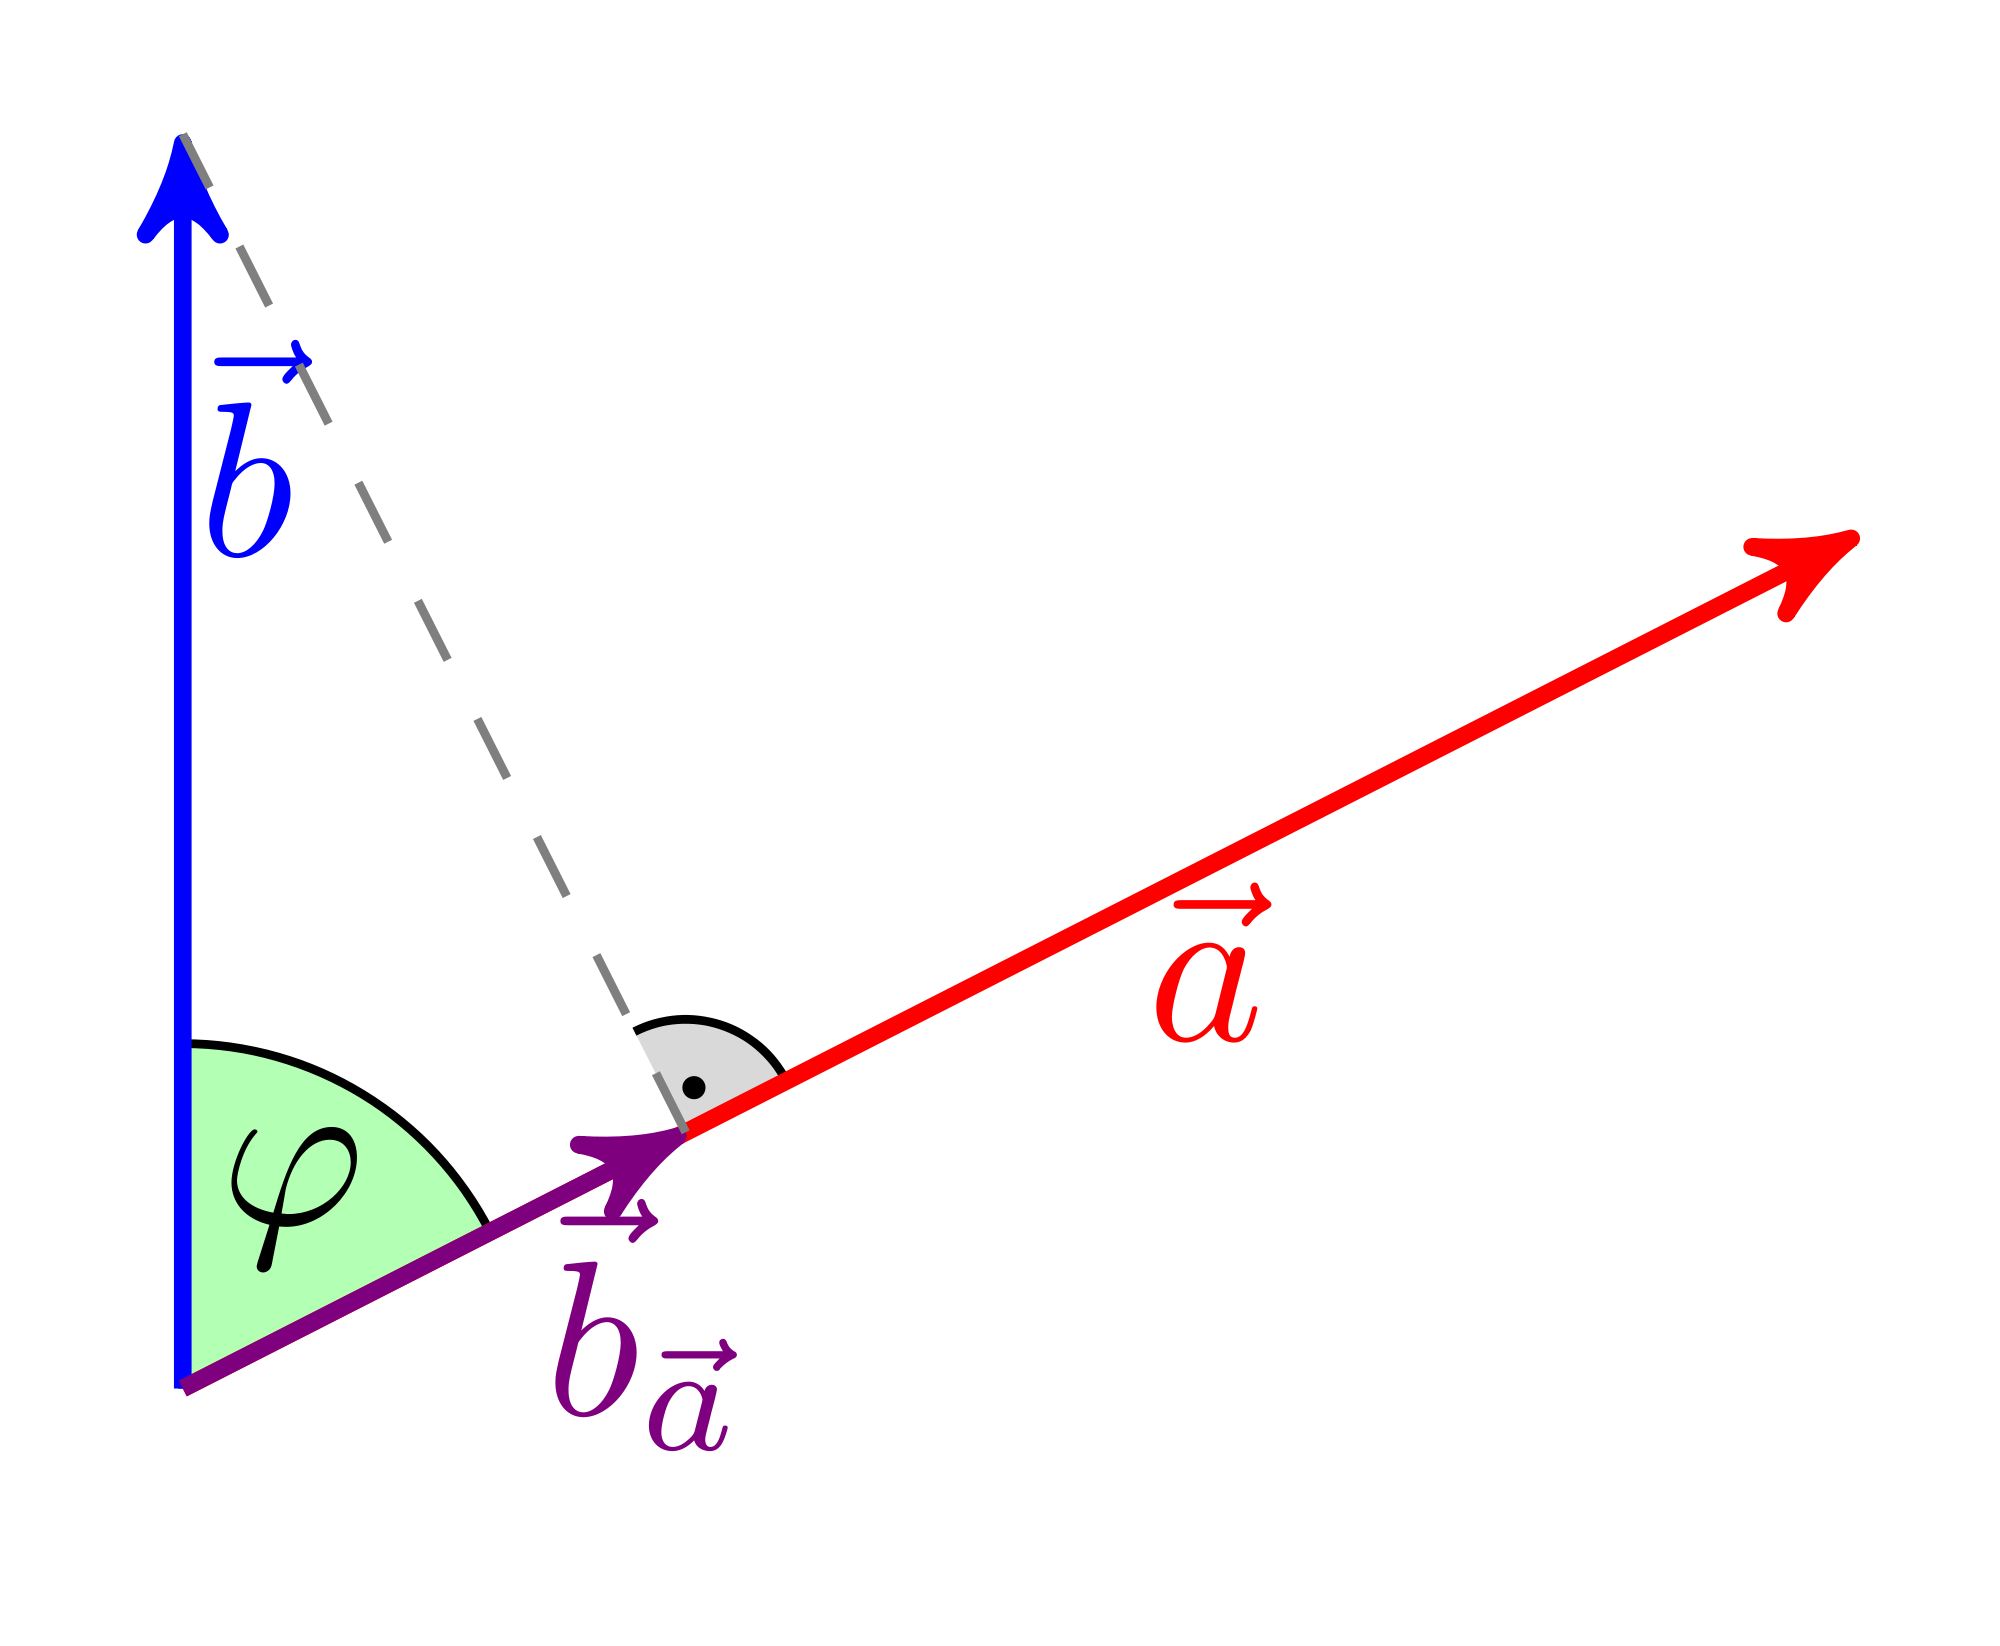
\includegraphics[width=200pt]{Abbildungen/vektorProjektion.png}
	\caption{Vektor Projektion zum berechnen der tangentialen Beschränkung (platzhalter für richtiges Bild)}
	\label{fig:vektorProjektion}
\end{figure}

Für diese Beschränkung können sich die Räder des Fahrzeuges über den Rand hinaus bewegen. Soll dies verhindert werden, muss diese Beschränkung auf jedes der einzelnen Räder erweitert werden.

Im letzten Schritt, bevor der \ac{MPC}-Algorithmus funktionsbereit ist, muss der Fahrzeugzustand des aktuellen Zeitschritts $t_0$ als Beschränkung verankert werden.  Dies ist nötig um zu verhindern, dass der Optimierer einfach die \(x\)-, und \(y\)-Position auf einen Punkt legt, welcher die Kostenfunktion ideal minimiert. 

\subsubsection*{Suchbereichsbeschränkung}
Während dem Testen der Kostenfunktion zum Maximieren der Geschwindigkeit ist das Phänomen aufgetreten, dass der Optimierer augenscheinlich, unmögliche Lösungen gefunden hat bei denen sich das Rennauto links aus einer Rechtskurve und andersherum, herausbewegt. Dies passiert jedoch nur in Kurven die mehr als $90°$ aufweisen. Der Grund hierfür liegt in den tangentialen Beschränkungen und dass sie immer nur am Anfang des MPC-Zyklus aktualisiert werden. Werden die Tangenten wie in Abbildung \ref{fig:curveAnomaly} sehr lang eingezeichnet, ist ersichtlich, dass eine zweite mögliche Trajektorie entstehen kann welche eine höhere Geschwindigkeit ermöglicht. Bei der Berechnung der tangentialen Beschränkung für den nächsten MPC-Durchlauf liegen jetzt jedoch alle Tangen nahezu auf einem Punkt und verhindern daher das Ausscheren des Rennautos. Die daher entstehende neue optimale Trajektorie entspricht wieder nahezu der ursprünglichen. Es entsteht also ein 3er Zyklus, welcher im schlechtesten Fall solange durchlaufen wird, bis das Fahrzeug eine Tangente trifft und die Optimierung beendet wird da keine weitere mögliche Lösung gefunden werden kann.\\
Um dieses Verhalten zu verhindern, wird für diese Kostenfunktion eine zusätzliche Suchbereichsbeschränkung eingeführt. Diese legt um die Prädiktionsschritte der letzten Optimierung einen Kreis, welcher den Suchbereich so einschränkt, dass keine neue Trajektorie entstehen kann. Es ist darauf zu achten, dass das Fahrzeug trotzdem in den Grenzen seines Fahrzeugmodells keine Beschränkung erfährt. 


\begin{figure}[ht!]
	\centering
	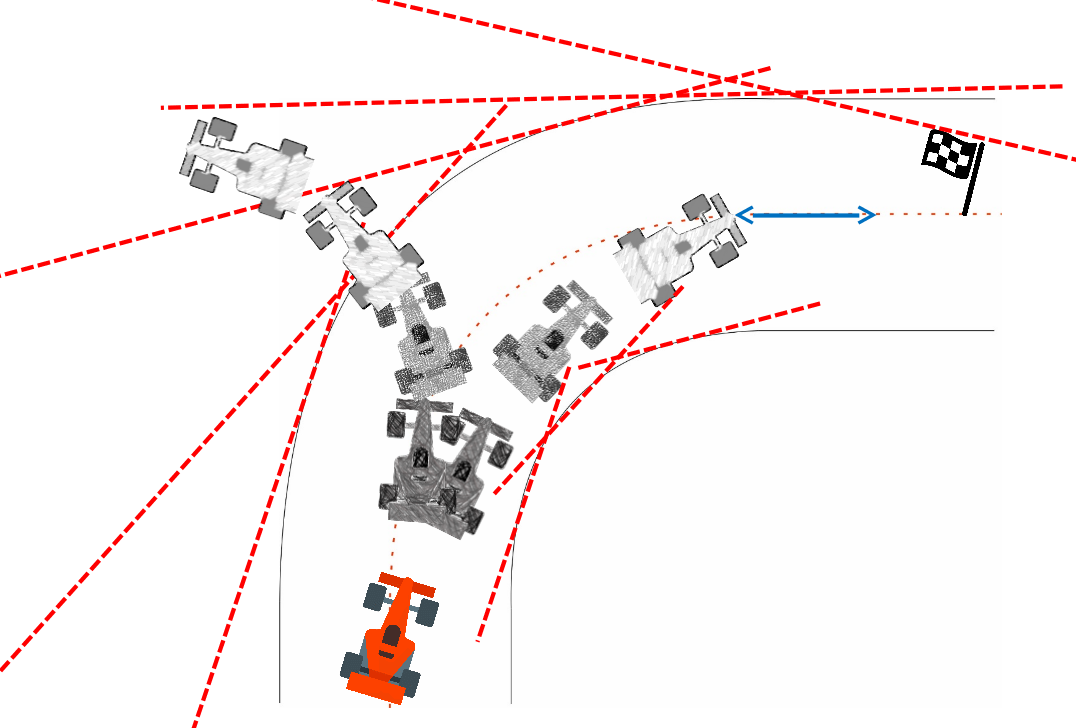
\includegraphics[width=200pt]{Abbildungen/curveAnomaly.png}
	\caption{Fehlerhaftes Verhalten in Spitzkurven}
	\label{fig:curveAnomaly}
\end{figure}


\subsubsection*{Elastische Distanzminimierung}
Der Nachteil beider oben aufgeführten Kostenfunktionen ist, dass sie keinen Spielraum beim Erfüllen der Streckenbeschränkung haben. In der Simulationsumgebung kann, wenn sowohl das im Simulator wie auch im \ac{MPC} hinterlegte Fahrzeugmodell exakt gleich ist, das virtuelle Rennauto bis an die Streckenbegrenzung heranfahren, ohne dass die Optimierung unlösbar wird. In der Realität würde eine solche Kostenfunktion das Fahrzeug jedoch zu nah an die Pylonen heranführen. Bei nur dem kleinsten Regelfehler, Rutschen, Abweichungen vom Fahrzeugmodell etc. würde sich der initiale Fahrzeugzustand $\vec{x}_0$ bereits außerhalb der Beschränkungen befindet und damit keine Lösung mehr für das Optimierungsproblem möglich sein. Um dieses Problem zu umgehen, wird eine neue Art der Kostenfunktion eingeführt, welche die Ungleichheitsbedingung der Streckenbegrenzung ersetzt. Die elastische Kostenfunktion. Hier wird eine der oberen Funktionen durch einen Kostenanteil erweitert, der wächst, sobald sich das Fahrzeug vom Mittelpunkt der Fahrbahn nach außen hin bewegt. Das Verhältnis der beiden Kostenfunktionen wird über die Gewichtungsvariablen \(a\) und \(b\) gesteuert.\\
$f(\vec{x}) = a (\sum_{1}^{N+1} v_i) + b(\sum_{1}^{N+1} g(h(\vec{x}_i)))$  \\
Die Funktion $g(d)$ dient hier als Platzhalter für verschiedene Gewichtungsfunktionen. Die Funktion $h(\vec{x}_i)$ berechnet die Distanz \(d\) vom Mittelpunkt der Strecke genauso wie bei den tangentialen Beschränkungen in Abschnitt \ref{trackAndPosConstraint}. Mögliche Funktionen sind:

\begin{eqnarray}
	g(d) = &\alpha d^2 \\
	g(d) = &\alpha |d|\\
	g(d) = &e^{\alpha (k_1 + d)} + e^{-\alpha(k_2 + d)} \label{eq:distMeasure1}\\
	g(d) = &|\frac{\alpha}{k_1-d} + \frac{\alpha}{k_2 - d}| \label{eq:distMeasure2}
\end{eqnarray}
Die Parameter $\alpha$, $k_1$ und $k_2$ dienen zum variieren der Scheitelpunkte und Steigung.
Mögliche Graphen der Gleichungen sind zu Veranschaulichung in Abbildung \ref{fig:elasticCost} dargestellt.

\begin{figure}[ht!]
	\centering
	
\begin{tikzpicture}
\begin{axis}[
width = 0.8\textwidth,
xmin= -3,
xmax= 3,
ymax = 50,
ylabel=Kosten,
xlabel=Distanz von der Mitte in m]

\addplot [color=blue, mark=none, line width=0.5mm] table [x index=0, y index=2]{Data/costFunct.dat};
\addplot [color=green, mark=none, line width=0.5mm] table [x index=0, y index=3]{Data/costFunct.dat};
\addplot [color=orange, mark=none, line width=0.5mm] table [x index=0, y index=4]{Data/costFunct.dat};

\addlegendentry{Quadratische-Funktion};
\addlegendentry{Alpha-Funktion};

\addlegendentry{E-Funktion};

\end{axis}
\end{tikzpicture} 
	\caption{Verschiedene Distanzmaße um das Verhalten der Trajektionsplanung zu beeinflussen.}
	\label{fig:elasticCost}
\end{figure}

Die Idee hinter den Funktionen \ref{eq:distMeasure1} und \ref{eq:distMeasure2} ist, dass das Rennauto sich uneingeschränkt auf der ganzen Breite der Strecke bewegen kann, ohne dass die Distanzfunktion eine größere Rolle spielt. Erst beim Erreichen des Fahrbahnrandes werden die Kosten sehr schnell extrem groß. Idealerweise stellen also diese Kostenfunktionen die tangentialen Begrenzungen ideal nach. 



\chapter{Simulationsumgebung}
Um die Funktion des \ac{MPC}-Algorithmus verifizieren zu können wurde eine Simulationsumgebung entwickelt. Der Aufbau ist dreigeteilt. Eine Fahrzeugsimulation welche mit austauschbaren Fahrzeugmodellen die Bewegung des Rennautos abhängig von Steuereingaben und einem $\Delta t$ berechnet. Der Regelanteil in Form des \ac{MPC} und eine Visualisierung auf Basis einer Spieleengine welche auch die zeitlichen Abläufe kontrolliert. 


\begin{figure}[ht!]
	\centering
	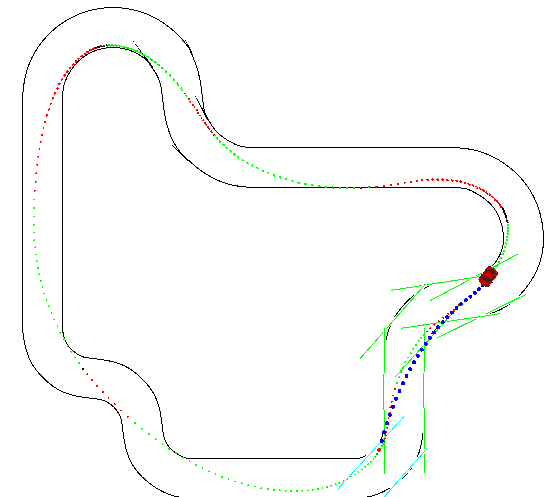
\includegraphics[width=350pt]{Abbildungen/sim_visual.png}
	\caption{Grafische Darstellung des MPC - Algorithmus in der Simulationsumgebung}
	\label{fig:jumpDiagram}
\end{figure}

\section{\acl{SFML}}
Die Basis für die Simulation bildet die \emph{ \ac{SFML}} welche für die grafische Darstellung des Kurses, Rennauto, Prädiktionsschritte und Fahrzeuginformationen genutzt wird. Gleichzeitig zur Visualisierung stellt die Spieleengine auch sicher, dass die zeitlichen Abläufe eingehalten werden. Das Grundprinzip ist eine einzige unendlich laufende Schleife die mit einer vorher festgelegten Häufigkeit pro Sekunde (frames per second fps) ausgeführt wird. Benötigen die Berechnungen innerhalb dieser Schleife länger als das angegebenen $\Delta t = \frac{1}{fps}$ sinkt die Ausführungsrate, überschritten wird sie jedoch nie. Die Schritte, die innerhalb dieser Schleife abgearbeitet werden sind zuerst das Abfragen möglicher Eingaben des Nutzers oder \emph{events} der einzelnen Objekte, z.b. eine Kollision. Im zweiten Schritt werden alle Berechnungen der eigentlichen Fahrzeugsimulation und \ac{MPC} ausgeführt und im letzten Schritt werden die grafische Elemente erstellt und angezeigt. Wie für eine Spieleengine üblich, befindet sich der Ursprung des Koordinatensystems in der linken oberen Ecke, die y-Achse ist daher entgegengesetzt zu dem in der Fahrzeugsimulation verwendeten Standardachsenaufbau orientiert. Zudem werden Distanzen in der Engine nur in Pixeln gemessen. Es wurden daher 2 Parameter eingeführt welche die Fenstergröße in Pixeln festlegen (in \(x\)- und  \(y\)-Richtung)
und zusätzlich eine Angabe wie viel Metern dieser Pixelbereich jeweils entspricht. Die daraus resultierenden Verhältnisse \\
$scaleX = \frac{windowSizeXinPixel}{windowSizeXinM}$ \\
$scaleY = - \frac{windowSizeYinPixel}{windowSizeYinM}$ \\
werden verwendet, um alle Größenverhältnisse einheitlich in der Simulation zu halten und eine realistische Visualisierung zu gewährleisten. Durch die Parameter kann nun bequem die Größe des Bereichs, in dem der Rennkurs abgesteckt wird und die Fenstergröße, zur Darstellung der Simulation, angepasst werden. Zusätzlich wurde ein Offset eingeführt welcher die Null-Position der \(x\)- und \(y\)- Position im Koordinatensystem verschiebt. Damit kann der Ursprung des Koordinatensystems der Fahrzeugsimulation beliebig im Anzeigebereich verschoben werden. 
Der Aufbau ist in dem Blockdiagramm \ref{fig:block_diagram_sim} nochmals zusammengefasst. 


\begin{figure}[ht!]
	\centering
	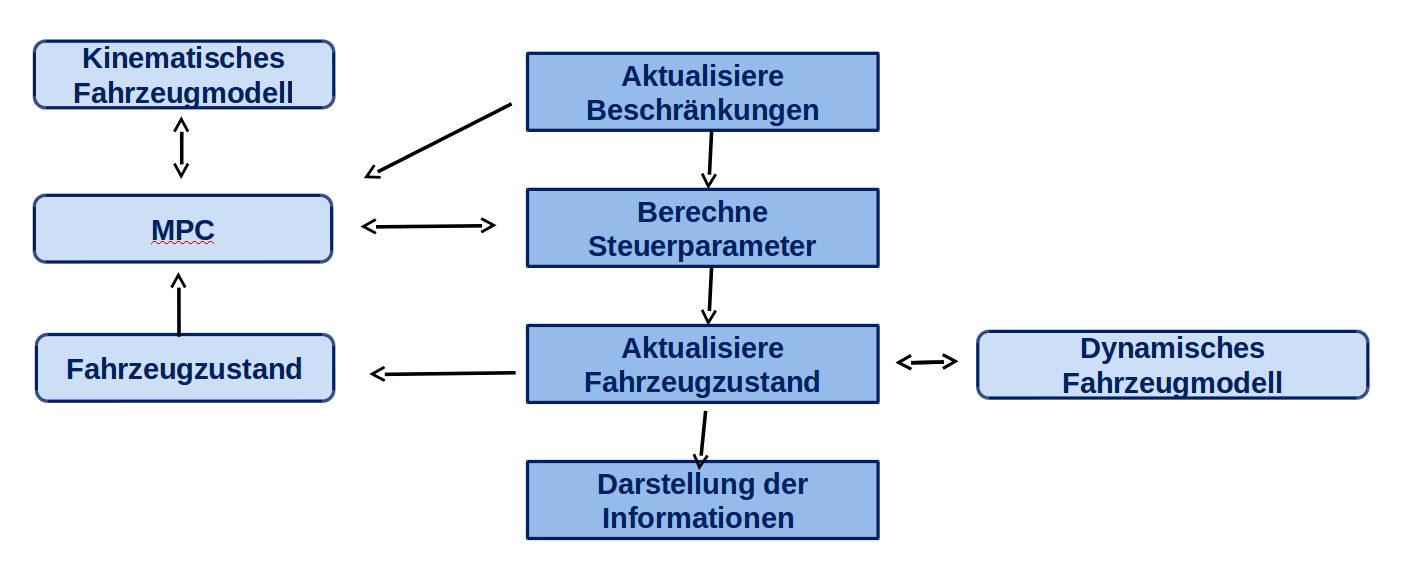
\includegraphics[width=350pt]{Abbildungen/sim_for_loop.png}
	\caption{Blockdiagramm der Simulation ohne MPC}
	\label{fig:block_diagram_sim}
\end{figure}


\section{Trackdrive}
Wie in der Einführung bereits erwähnt, ist das Ziel der Arbeit ein \ac{MPC}-Alogrithmus zu entwickeln mit dem die \emph{trackdrive} Disziplin möglichst schnell abgefahren werden kann. Die Grundvoraussetzung für diese Arbeit ist die bereits vollständig erstellte Karte des Rennkurses und eine Lokalisierung innerhalb dieser Karte. Die Updaterate für diese Positionsschätzung wird mit 20 Hz angenommen. Das Ziel ist es also die Regelparameter mit einem $\Delta t$ von $\frac{1}{20} s$ für das Rennauto berechnen zu können.  Zum Testen der Algorithmen wurde ein beliebiger Kurs definiert, welcher sich an die Vorgaben des Regelwerkes hält und damit einen minimalen Kurvenradius von 9 m, Maximallänge einer Geraden von 80m und maximal 180° Spitzkurven besitzt.

\chapter{Evaluierung}
Im folgenden Abschnitt werden zuerst die Fahrzeugmodelle mit Fahrsituationen evaluiert, für welche genaue Testdaten des High Octane Motorsports Rennautos aus dem Jahr 2017 bekannt sind. 
Nachdem sichergestellt wurde dass die Modelle nahe genug der Realität entsprechen wurden die verschiedenen Kostenfunktionen untersucht. Dieser Teil der Arbeit geht fließend in die Untersuchung der Regelbarkeit des Rennautos über, wenn im MPC-Algorithmus nur ein kinematisches Modell verwendet wird.

\section{Verifizierung der Fahrzeugmodelle}
Ohne eine genaue Verifizierung der Plausibilität der implementierten Modelle ist keine systematische Untersuchung möglich. Hierfür wurden die zwei Disziplinen \text{acceleration} und \text{skidpad} gewählt und die besten gefahrenen Ergebnisse des Events 2017 in Hockenheim als Basis gewählt.
Der \ac{MPC}-Algorithmus wurde mit 10 Prädiktionsschritten und der Kostenfunktion für maximale Geschwindigkeit durchgeführt, da hierfür  

\subsubsection*{Acceleration}
In dieser Disziplin ist es das Ziel der Teams eine 75m lange, gerade Strecke in möglichst kurzer Zeit zurückzulegen.
Es werden drei verschiedene longitudinale Konfigurationen des Fahrzeugmodells evaluiert. Zuerst das kinematische Modell in dem die maximale mittlere Beschleunigung aus den Fahrzeugdaten wie in \ref{long_acc_kin} beschrieben errechnet wird. Das zweite untersuchte Modell basiert auf der Leistung des Motors und der maximal übertragbaren Kraft der Reifen (\ref{long_dyn_engine}).
Das genaueste Modell betrachtet zusätzlich noch Reibung und Luftwiderstand. 


\begin{figure}
	\centering
	\pgfplotstabletypeset{Grafiken/accdec.dat}



\begin{tikzpicture}
\begin{axis}[
xlabel=Q Series,
ylabel=P Values]
\addplot table [y=P, x=$Q1$]{data.dat};

\end{axis}
\end{tikzpicture} 
	\caption{Beschleunigung für verschiedene longitudinale Modelle}
	\label{fig:accdec}
\end{figure}

In der Grafik \ref{fig:accdec} wird deutlich, wie stark sich die einzelnen Modelle, obwohl sie sich auf das gleiche Fahrzeug beziehen voneinander unterscheiden. Für alle Modelle wird 7.5 s lang maximal beschleunigt und danach 2.5 s mit maximaler Kraft gebremst. Das Fahrzeug besitzt eine Maximalgeschwindigkeit von 118 kmh, welche durch die Übersetzung im Getriebe herrührt. Das kinematische Modell trifft mit seiner durchschnittlichen Beschleunigung exakt die gefahrenen Testwerte. Da aber die dynamischen Modelle eine größere Anfangsbeschleunigung haben und vom kinematischen Model, hinterlegt im MPC, geregelt werden, wird die Beschleunigung im kinematischen Modell so angepasst, dass es die gleiche Anfangssteigung besitzt.

\subsubsection*{Skidpad}
In dieser Disziplin fährt das Fahrzeug eine liegende 8. Der limitierende Faktor ist hier also die maximale Querbeschleunigung welche das Rennauto noch auf dem Kurs hält. In der Simulation wird vereinfacht von einem Rundkurs, welcher in Abbildung \ref{fig:roundCourse} dargestellt wird, mit dem Außendurchmesser von 21.25 m ausgegangen. Ob die Begrenzung der Querbeschleunigung \ref{betaMax} mit der Simulation übereinstimmt kann durch die Zentripetalkraft, welche wirkt, überprüft werden.

$ \omega = 2 \pi f$ \\
$ v = r * \omega $\\
$a = \frac{v^2}{r}$\\

Für das in der Simulationsumgebung hinterlegtes kinematisches Modell ist die gemessene Rundenzeit 4.65 s. Daraus lässt sich eine Durchschnittsgeschwindigkeit $ v= 13.9 \frac{m}{s}$ berechnen, was einer Querbeschleunigung von $a = 19.37 \frac{m}{s}$ entspricht. Das im Fahrzeugmodell hinterlegte $a_{max}$ ist mit 19.62  also sehr nah an dem in der Simulation erfahrenen werten. Die Differenz zu der schnellsten gemessenen Runde mit dem echten Fahrzeug (7.5 s) lässt sich dadurch erklären, dass der MPC-Algorithmus die ideale Stellgrößen berechnet und damit auch einen idealen Rundkurs abfährt. Zudem wurde die maximal gemessene Querbeschleunigung des Fahrzeugs als $a_max$ gewählt, dies kann in der Realität nicht durchgängig gehalten werden kann.
Für das dynamische Fahrzeugmodell wurde eine minimale Rundenzeit 4.45 s gemessen.  Die damit erhaltene maximale Querbeschleunigung ist nur 5  größer als die des kinematischen Models.  

\begin{figure}
	\centering
	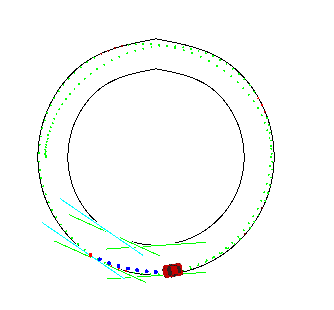
\includegraphics[width=200pt]{Abbildungen/roundCourse.png}
	\caption{Rundkurs zum messen der maximalen Querbeschleunigung}
	\label{fig:roundCourse}
\end{figure}


\section{Regelung des kinematischen Modells im Rennkurs}
In diesem Kapitel wird untersucht mit welcher Kostenfunktion die besten Rundenzeiten erreicht werden können. Zudem wir erprobt, wie groß der Einfluss des Vorhersagehorizontes auf die gefahrene Zeit ist. Um dies tun zu können, muss zuerst die mindestens erforderliche länge des Prädiktionshorizontes gefunden werden. In einem Szenario im öffentlichen Verkehr muss der Horizont immer mindestens so lang sein, dass eine Vollbremsung von der aktuellen Geschwindgkeit durchgeführt werden kann, bevor das Fahrzeug das Ende des Horizont erreicht hat. Auf dem Rennkurs ist dies nicht nötig, da hier nicht davon auszugehen ist, dass sich plötzlich Hindernisse auf der Strecke befinden (bei Formula Student Driverless befindet sich immer nur ein Fahrzeug auf der Strecke). Da im Simulator und im \ac{MPC} das gleiche Fahrzeugmodell hinterlegt ist, wird die tangentiale Beschränkung genutzt um das Rennauto daran zu hindern die Strecke zu verlassen.

\subsection{Prädiktionshorizont} 
Um die Mindestlänge zu finden, wurde die Fahrsituation nachgestellt, welche nach Regelwerk den stärksten Bremsvorgang und Querbeschleunigung erzeugt. Eine 80 m lange Gerade mit zwei angehängten 180 Grad Kurven mit 9 m Innenradius. Das Ergebnis ist ein Prädiktionsvektor von 17 Schritten für den die geringste Geschwindigkeit in der kurve 36.72 kmh gemessen wurde. Die höchste auf der geraden erreichte Geschwindigkeit beträgt 85.32 kmh was einer Differenz von 48.6 kmh entspricht. Mit der im kinematischen Model hinterlegten maximalen Verzögerung kann das Fahrzeug in einer Sekunde 47.2 kmh abbremsen. Die 17 Zeitschritte entsprechen 0.85 s. Der Zusammenhang aus Bremsleistung und maximaler Kurvengeschwindigkeit ist also klar ersichtlich. 

\subsection{Kostenfunktionen}
Mit der Information wie groß der geringsten Prädiktionshorizont sein muss, wird nun untersucht wie die unterschiedlichen Kostenfunktionen gegeneinander abschneiden. Um eine gute Vergleichbarkeit zu erhalten wird ein zufälliger Rennkurs erstellt auf dem die Messungen durchgeführt werden. Im Kapitel werden die tangentialen Beschränkungen durch elastische Beschränkungen ersetzt, welche wie im Abschnitt \ref beschrieben in die Kostenfunktion integriert werden. Um einen möglichst guten Vergleich bilden zu können, werden die idealen Parameter für diese Kostenfunktionen zuerst das kinematische Modell gesucht. Das Ziel ist eine ähnliche Rundenzeit ohne dass das Rennauto den Kurs verlässt. 
\subsubsection*{Laufzeit}
Zuerst wird die Berechnungszeit für alle drei Kostenfunktionen verglichen. 
Die Geschwindigkeit wurde auf 7 $\frac{m}{s}$ limitiert um auch kleinere Horizonte testen zu können. Die Ergebnisse der Messung sind im Benchmark \ref{fig:computeCost} visualisiert. 


Die Berechnung des initialen Optimierungsvektor dauert im Vergleich zu allen darauf folgenden Schritten extrem lange. Dies liegt an dem so genannten \emph{hot start}. Solange die Parameter der Beschränkungen (neue Tangenten und neue Startposition) nicht signifikant verändert werden, findet der Optimierer in aufeinander folgenden Schritten sehr schnell eine passende Lösung. Dies kann man sich wie in einem shift Register vorstellen, in dem die Lösung nur einen Schritt nach links verschoben wird.
Bei einem Vorhersagehorizont von 110 Schritten  brauchen zum Beispiel die ersten 10 Schritte über 6 s zum Berechnen, danach nur noch im Schnitt 0.1 s

\begin{figure}
	\centering
	
\begin{tikzpicture}
\begin{axis}[
width = 0.8\textwidth,
height = 0.6\textwidth,
xmin= 0,
xmax= 110,
ymin= 0,
ymax= 0.5,
xlabel=Prädiktionsschritte,
ylabel=Berechnungszeit in s,
legend pos=north west]
\addplot [color=red, dashed, mark=none, line width=0.5mm] table [x index=0, y index=1]{Data/compTimeHorizon.dat};
\addplot [color = red,mark=none, line width=0.5mm] table [x index=0, y index=2]{Data/compTimeHorizon.dat};

\addplot [color=blue, dashed, mark=none, line width=0.5mm] table [x index=0, y index=3]{Data/compTimeHorizon.dat};
\addplot [color=blue, mark=none, line width=0.5mm] table [x index=0, y index=4]{Data/compTimeHorizon.dat};

\addplot [color=green, dashed, mark=none, line width=0.5mm] table [x index=0, y index=5]{Data/compTimeHorizon.dat};
\addplot [color=green, mark=none, line width=0.5mm] table [x index=0, y index=6]{Data/compTimeHorizon.dat};

\addplot [dashed, mark=none] coordinates {(0, 0.05) (110, 0.05)};

\addlegendentry{min dist};
\addlegendentry{m.d. ohne init};

\addlegendentry{max speed};
\addlegendentry{m.s. ohne init};

\addlegendentry{max dist};
\addlegendentry{m.d ohne init};

\end{axis}
\end{tikzpicture} 
	\caption{Berechnungszeit für verschiedene Kostenfunktionen mit und ohne die ersten 40 von 240 Berechnungen}
	\label{fig:computeCost}
\end{figure}

\subsubsection*{Rundenzeit}
Um die Qualität der Kostenfunktionen einschätzen zu können wird im folgenden Untersucht, wie schnell die einzelnen Rundenzeiten abhängig von den Prädiktionsschritten für jede einzelne Funktion ist.
Gemessen wurde sowohl die erste und zweite Runde, da in der ersten Runde die Anfangsbeschleunigung und die eventuell ungünstige Startposition die Rundenzeit beeinträchtigen. Es wurde auch jeweils noch eine dritte Rundenzeit ermittelt, diese entspricht aber nahezu genau der zweiten.

\begin{figure}
	\centering
	
\begin{tikzpicture}
\begin{axis}[
width = 0.8\textwidth,
height = 0.6\textwidth,
xmin= 20,
xmax= 50,
ymin= 7,
ymax= 15,
xlabel= Prädiktionsschritte,
ylabel=Rundenzeit s,
legend pos=north west]
\addplot [color=red, dashed, mark=none, line width=0.5mm] table [x index=0, y index=1]{Data/lapTimeKin.dat};
\addplot [color = red,mark=none, line width=0.5mm] table [x index=0, y index=2]{Data/lapTimeKin.dat};

\addplot [color=blue, dashed, mark=none, line width=0.5mm] table [x index=0, y index=4]{Data/lapTimeKin.dat};
\addplot [color=blue, mark=none, line width=0.5mm] table [x index=0, y index=5]{Data/lapTimeKin.dat};

\addplot [color=green, dashed, mark=none, line width=0.5mm] table [x index=0, y index=7]{Data/lapTimeKin.dat};
\addplot [color=green, mark=none, line width=0.5mm] table [x index=0, y index=9]{Data/lapTimeKin.dat};

\addplot [dashed, mark=none] coordinates {(20, 8.3) (50, 8.3)};


\addlegendentry{min dist(1)};
\addlegendentry{min dist(2)};

\addlegendentry{max dist (1)};
\addlegendentry{max dist (2)};

\addlegendentry{max speed(1)};
\addlegendentry{max speed(2)};




\end{axis}
\end{tikzpicture}


 
	\caption{}
	\label{fig:lapTimeKin}
\end{figure}

Das Verhalten der Kostenfunktion, welche die Geschwindigkeit maximiert, mit längerer vorrausprädiktion immer langsamer zu werden, lässt sich mit dem Wissen über den Kurs erklären. Desto weiter in die Zukunft der Optimierer schauen kann, desto mehr fängt er an Kurven voll auszufahren, also den zurückgelegten Weg länger zu planen. Dadurch kann zwar die Geschwindigkeit erhöht werden, die Rundenzeit leider allerdings deutlich darunter. 
Die Differenz zwischen den beiden Kostenfunktionen, welche die Distanz zu einem Punkt bzw die gefahrene Streckendistanz maximieren, ist sehr klein und auch bei geringeren Horizontlängen bereits sehr gut. Betrachtet man jedoch zusätzlich die Berechnungszeit setzt sich die Kostenfunktion zur maximierung der Streckendistanz deutlich als die Beste ab.



\section{Regelung des dynamischen Modells im Rennkurs}
In der Realität ist das kinematische Modell nur für geringe Geschwindigkeiten genau genug die Bewegung des Fahrzeugs zu Modellieren. Im Folgenden wird deswegen das Modell im Simulator durch ein dynamische Fahrzeugmodell mit berechneten Reifenkräften ersetzt und evaluiert, wie gut sich das deutlich komplexere System mit dem weiterhin sehr einfachen kinematischen Modell im \ac{MPC}-Algorithmus regeln lässt. 
Zuerst wird untersucht, ab welchen Geschwindigkeiten die Abweichung zwischen den Modellen signifikant wird. Danach werden die einzelnen elastischen Begrenzung auf ihre Fähigkeit getestet das dynamische Modell auf dem Kurs zu halten und welche Rundenzeiten sie ermöglichen. Im letzten Schritt wird zusätzlich noch untersucht welchen Einfluss $\beta_{max}$ auf die Regelfähigkeit des Algorithmus hat und ob sie sich durch verändern der Werte verbessern lässt. 
\subsection{Modellfehler}
Um zu verdeutlichen, warum für hohe Geschwindigkeiten ein kinematisches Modell nicht mehr ausreichend ist, werden im folgenden die Modellfehler betrachtet. 

\subsubsection*{Orientierung}
Bei einer rein longitudinalen oder konstanten lateralen Bewegung ist, wie im vorherigen Kapitel schon gezeigt wurde, die Differenz der einzelnen Fahrzeugmodelle nicht groß. Bei dynamischeren Szenarien werden die Unterschiede dahingegen deutlich sichtbar. Im Plot \ref{fig:modelDiffOrient} ist für ein oszillierenden Lenkwinkel die Änderung der Orientierung geplottet. Erst ohne longitudinale Beschleunigung und im zweiten Plot mit maximaler Beschleunigung zusätzlich zur Lenkwinkeländerung 

\begin{figure}
	\centering
	
\begin{tikzpicture}
\begin{axis}[
height = 0.20\textwidth,
width = 0.465\textwidth,
xmin= 0,
xmax = 2.0,
ymin = -0.6,
ymax = 0.6,
xlabel= Zeit in s,
ylabel=Lenkwinkel in rad,
legend pos=north west]
\addplot [color=black, mark=none, line width=0.5mm] table [x index=0, y index=1]{Data/modelDiffOrient/modelDiffOrientNoAcc7.dat};
\end{axis}
\end{tikzpicture}%NOLINE
\begin{tikzpicture}
\begin{axis}[
width = 0.465\textwidth,
height = 0.20\textwidth,
xmin= 0,
xmax = 2.0,
ymin = -0.6,
ymax = 0.6,
xlabel= Zeit in s,
ylabel=Lenkwinkel in rad,
legend pos=north west]
\addplot [color=black, mark=none, line width=0.5mm] table [x index=0, y index=1]{Data/modelDiffOrient/modelDiffOrientNoAcc7.dat};
\addplot [dashed, mark=none] coordinates {(0.5, -0.8) (0.5, 0)};
\end{axis}
\end{tikzpicture}


\begin{tikzpicture}
\begin{axis}[
width = 0.47\textwidth,
xmin= 0,
xmax = 2.0,
ymin = 0.0,
ymax= 0.8,
xlabel= Zeit in s,
ylabel= Orientierung in rad,
legend columns = 3,
legend entries = {kin. Modell;,dyn. Modell;, dyn. mit K.K.},
legend to name =modelDiffOrientLegend
]
\addplot [color=red, mark=none, line width=0.5mm] table [x index=0, y index=2]{Data/modelDiffOrient/modelDiffOrientNoAcc7.dat};
\addplot [color=blue, mark=none, line width=0.5mm] table [x index=0, y index=3]{Data/modelDiffOrient/modelDiffOrientNoAcc7.dat};
\addplot [color=green, dashed, mark=none, line width=0.5mm] table [x index=0, y index=4]{Data/modelDiffOrient/modelDiffOrientNoAcc7.dat};

\end{axis}
\end{tikzpicture}%NOLINE
\begin{tikzpicture}
\begin{axis}[
width = 0.47\textwidth,
xmin= 0,
xmax = 2.0,
ymin = 0.0,
ymax= 0.8,
xlabel= Zeit in s,
ylabel= Orientierung in rad,
legend pos=north west]
\addplot [color=red, mark=none, line width=0.5mm] table [x index=0, y index=2]{Data/modelDiffOrient/modelDiffOrientNoAcc14.dat};
\addplot [color=blue, mark=none, line width=0.5mm] table [x index=0, y index=3]{Data/modelDiffOrient/modelDiffOrientNoAcc14.dat};
\addplot [color=green, dashed, mark=none, line width=0.5mm] table [x index=0, y index=4]{Data/modelDiffOrient/modelDiffOrientNoAcc14.dat};

\end{axis}
\end{tikzpicture}

\begin{tikzpicture}
\begin{axis}[
width = 0.47\textwidth,
xmin= 0,
xmax = 2.0,
ymin = 0.0,
ymax= 0.8,
xlabel= Zeit in s,
ylabel= Orientierung in rad,
legend pos=north west]
\addplot [color=red, mark=none, line width=0.5mm] table [x index=0, y index=2]{Data/modelDiffOrient/modelDiffOrientNoAcc21.dat};
\addplot [color=blue, mark=none, line width=0.5mm] table [x index=0, y index=3]{Data/modelDiffOrient/modelDiffOrientNoAcc21.dat};
\addplot [color=green,dashed,  mark=none, line width=0.5mm] table [x index=0, y index=4]{Data/modelDiffOrient/modelDiffOrientNoAcc21.dat};

\end{axis}
\end{tikzpicture}%NOLINE
\begin{tikzpicture}
\begin{axis}[
width = 0.47\textwidth,
xmin= 0,
xmax = 2.0,
ymin = 0.0,
ymax= 0.8,
xlabel= Zeit in s,
ylabel= Orientierung in rad,
legend pos=north west]
\addplot [color=red, mark=none, line width=0.5mm] table [x index=0, y index=2]{Data/modelDiffOrient/modelDiffOrientNoAcc28.dat};
\addplot [color=blue, mark=none, line width=0.5mm] table [x index=0, y index=3]{Data/modelDiffOrient/modelDiffOrientNoAcc28.dat};
\addplot [color=green,dashed,  mark=none, line width=0.5mm] table [x index=0, y index=4]{Data/modelDiffOrient/modelDiffOrientNoAcc28.dat};
\end{axis}
\end{tikzpicture}




 
	\caption{}
	\label{fig:modelDiffOrient}
\end{figure}

\begin{figure}
	\centering
	\begin{tikzpicture}
\begin{axis}[
width = 0.8\textwidth,
height = 0.34\textwidth,
xmin= 0,
xmax = 2.0,
xlabel= Zeit in s,
ylabel=Lenkwinkel in rad,
legend pos=north west]
\addplot [color=black, mark=none, line width=0.5mm] table [x index=0, y index=1]{Data/modelDiffOrientNoAcc.dat};
\end{axis}
\end{tikzpicture}

\begin{tikzpicture}
\begin{axis}[
width = 0.8\textwidth,
height = 0.34\textwidth,
xmin= 0,
xmax = 2.0,
ymin= -0.4,
ymax= 1.2,
xlabel= Zeit in s,
ylabel= Orientierung in rad,
legend pos=north west]
\addplot [color=red, mark=none, line width=0.5mm] table [x index=0, y index=2]{Data/modelDiffOrientmaxAcc.dat};
\addplot [color=blue, mark=none, line width=0.5mm] table [x index=0, y index=3]{Data/modelDiffOrientmaxAcc.dat};
\addplot [color=green, mark=none, line width=0.5mm] table [x index=0, y index=4]{Data/modelDiffOrientmaxAcc.dat};

\addlegendentry{kin. Modell};
\addlegendentry{dyn. Modell};
\addlegendentry{dyn. mit K.K.};
\end{axis}
\end{tikzpicture} 
	\caption{}
	\label{fig:modelDiffOrientMaxAcc}
\end{figure}


\subsubsection*{Position}


\begin{figure}
	\centering
	\begin{tikzpicture}
\begin{axis}[
width = 0.5\textwidth,
xlabel= x-Position in m,
ylabel= y-Position in m,
legend pos=north west]
\addplot [color=red, mark=none, line width=0.5mm] table [x index=0, y index=1]{Data/modelDiffTrajNoAcc.dat};
\addplot [color=blue, mark=none, line width=0.5mm] table [x index=2, y index=3]{Data/modelDiffTrajNoAcc.dat};
\addplot [color=green, mark=none, line width=0.5mm] table [x index=4, y index=5]{Data/modelDiffTrajNoAcc.dat};

\addlegendentry{kinematisch};
\addlegendentry{kinematisch};
\addlegendentry{K.K};

\end{axis}
\end{tikzpicture}% NO EMPTY LINE HERE!!!! 
\begin{tikzpicture}
\begin{axis}[
width = 0.5\textwidth,
xmin= 0,
xmax = 30,
ymin= 0,
ymax=16,
xlabel= Geschwindigkeit in m/s,
ylabel= Abweichung in m,
legend pos=north west]
\addplot [color=red, mark=none, line width=0.5mm] table [x index=0, y index=1]{Data/modelDiffPositionNoAcc.dat};
\addplot [color=blue, mark=none, line width=0.5mm] table [x index=0, y index=2]{Data/modelDiffPositionNoAcc.dat};
\addplot [color=green, mark=none, line width=0.5mm] table [x index=0, y index=3]{Data/modelDiffPositionNoAcc.dat};

\addlegendentry{kinematisch-dynamisch};
\addlegendentry{kinematisch-kamsch};
\addlegendentry{dynamisch-kamsch};

\end{axis}
\end{tikzpicture} 
	\caption{[links] Die zurückgelegte Trajektorie für den gleichen Input des Lenkwinkels wie in \ref{fig:modelDiffOrient} und einer Geschwindigkeit von 30 m/s. [rechts] Die Abweichung der Position zwischen den einzelnen Modellen und verschiedenen initialen Geschwindigkeiten. Keine Beschleunigung.}
	\label{fig:modelDiffPos}
\end{figure}


\begin{figure}
	\centering
	\begin{tikzpicture}
\begin{axis}[
width = 0.5\textwidth,
xlabel= x-Position in m,
ylabel= y-Position in m,
legend pos=north west]
\addplot [color=red, mark=none, line width=0.5mm] table [x index=0, y index=1]{Data/modelDiffTrajMaxAcc.dat};
\addplot [color=blue, mark=none, line width=0.5mm] table [x index=2, y index=3]{Data/modelDiffTrajMaxAcc.dat};
\addplot [color=green, mark=none, line width=0.5mm] table [x index=4, y index=5]{Data/modelDiffTrajMaxAcc.dat};
\end{axis}
\end{tikzpicture}% NO EMPTY LINE HERE!!!! 
\begin{tikzpicture}
\begin{axis}[
width = 0.5\textwidth,
xmin= 0,
xmax = 30,
ymin= 0,
ymax=16,
xlabel= Geschwindigkeit in m/s,
ylabel= Abweichung in m,
legend pos=north west]
\addplot [color=red, mark=none, line width=0.5mm] table [x index=0, y index=1]{Data/modelDiffPositionMaxAcc.dat};
\addplot [color=blue, mark=none, line width=0.5mm] table [x index=0, y index=2]{Data/modelDiffPositionMaxAcc.dat};
\addplot [color=green, mark=none, line width=0.5mm] table [x index=0, y index=3]{Data/modelDiffPositionMaxAcc.dat};
\end{axis}
\end{tikzpicture}
 
	\caption{[links] Die zurückgelegte Trajektorie für den gleichen Input des Lenkwinkels wie in \ref{fig:modelDiffOrient} und einer Geschwindigkeit von 30 m/s. [rechts] Die Abweichung der Position zwischen den einzelnen Modellen und verschiedenen initialen Geschwindigkeiten. Maximale Beschleunigung.}
	\label{fig:modelDiffPosMaxAcc}
\end{figure}

\subsection{Elastische Beschränkung}
\subsubsection*{Berechnungszeit in Ipopt}

\subsection{Einfluss der Geschwindigkeit und Beta Max}
Die Idee hinter dem verändern von $\beta_{max}$ ist die geringere Kurvengeschwindigkeit. Da die Querbeschleunigung von Kurvenradius und Geschwindigkeit abhängt, wird der \ac{MPC}-Algorithmus  in engen Kurven, für ein kleineres $\beta_{max}$, vorher stärker abbremsen. Die geringere Geschwindigkeit in der Kurve verkleinert die Differenz der zwei Modelle und sollte daher die Regelbarkeit erhöhen. Der Unterschied zu einer dauerhaften Verringerung der Geschwindigkeit ist, dass bei geraden Strecken wenig laterale Kräfte wirken und das Modell sich daher schneller bewegen kann ohne unkontrollierbar zu werden. 


\chapter[Ausblick]{Zusammenfassung und Ausblick}
\section{Dynamisches Fahrzeugmodell im MPC}
\section{Trajektionsregelung}
\section{Zweispurmodell}
\section{Zusammenfassung}



\appendix

%\chapter*{Anhang}
%\large{
%Anhang 1\par
%Anhang 2


% setzt die Bildunterschriften auf A1 (A=Anhang)
\renewcommand{\thefigure}{A\arabic{figure}} 
\chapter{Anhang}

\subsection*{Elektronischer Anhang }

\subsection*{Fahrzeugdaten}
\begin{figure}[hb!]
	\caption{Engine Power}
	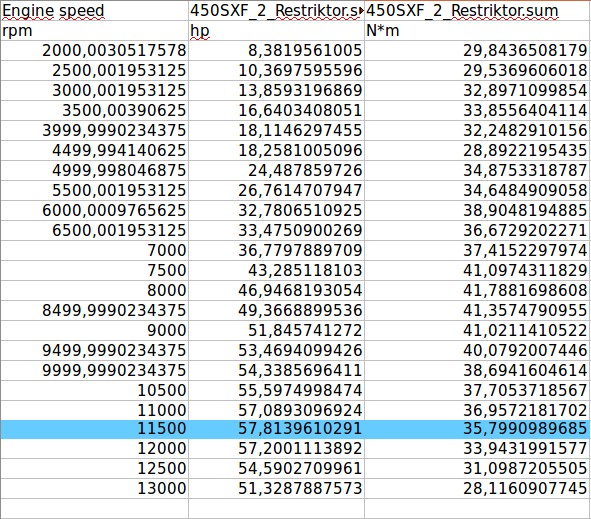
\includegraphics[width=350pt]{Abbildungen/Engine_power.png}
	\label{fig:enginePower}
\end{figure}

\begin{figure}[hb!]
	\caption{Max Tire Force}
	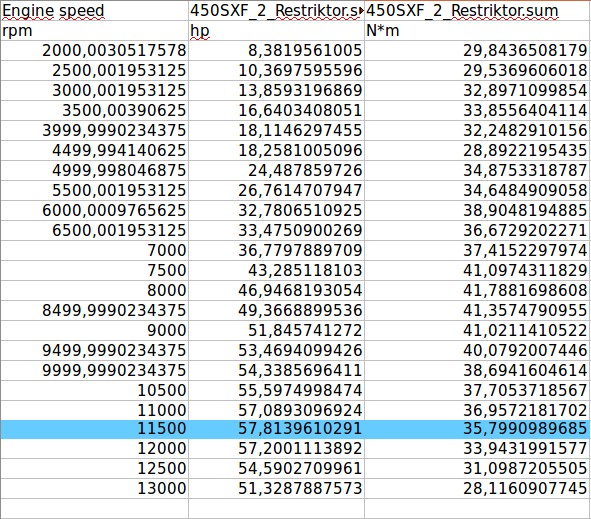
\includegraphics[width=350pt]{Abbildungen/Engine_power.png}
	\label{fig:maxTireForce}
\end{figure}



 \subsection*{Einbindung Grafik im Anhang}
  \begin{figure}[h!]
  \begin{centering}
  {
\includegraphics[width=0.33\textwidth]{Abbildungen/fau.png}}
   \caption{Unterschrift Bild x Die auf die Rotationsfrequenz des Innenzylinders normierten Eigenfrequenzen der gefun-denen Grundmoden der Taylor-Strömung für h(Die azimutale Wellenzahl ist mit m  bezeichnet.)}
  \end{centering}
  \end{figure}

\subsection{Code}

\begin{lstlisting}
[caption={ein paar Zeilen code}\label{lst:vehicleModel},captionpos=t] 
    for i in 0: N-1
    
    @NLexpression(m, x_dd, (VehicleModel.max_long_acc * x[8*i + 7]/10.0))
    
    @NLconstraints(m, begin
    x[(i + 1)*8 + 1] - (x[i * 8 + 1] + x[8*i + 3]*
    dt*cos(x[i*8 + 4] + atan(lr/(lf + lr) * tan(x[i*8 + 8])))) == 0
    x[(i + 1)*8 + 2] - (x[i * 8 + 2] + x[8*i + 3]*
    dt*sin(x[i*8 + 4] + atan(lr/(lf + lr) * tan(x[i*8 + 8])))) == 0
    x[(i + 1)*8 + 3] - (x[i * 8 + 3] + x_dd*dt) == 0
    x[(i + 1)*8 + 4] - (x[i * 8 + 4] + x[8*i + 3]*
    dt / lr*sin(atan(lr/(lf + lr) * tan(x[i*8 + 8])))) == 0
    atan(0.5 * (lf + lr) * mpc_struct.beta_max / x[i*8 + 3]^2)
    - atan(lr/(lf + lf) * tan(x[i*8 + 8])) >= 0  #max_beta - beta
    atan(0.5 * (lf + lr) * mpc_struct.beta_max / x[i*8 + 3]^2)
    + atan(lr/(lf + lf) * tan(x[i*8 + 8])) >= 0  #max_beta + beta
    end)
    end
\end{lstlisting}







%Abkürzungsverzeichnis
%\pagestyle{scrheadings}
%\chapter*{Abkürzungsverzeichnis}

\chapter*{Abkürzungsverzeichnis}
\addcontentsline{toc}{chapter}{Abkürzungsverzeichnis} %Abkürzungsverzeichnis kommt ins InhaV.





\begin{acronym}[SEPSEP] 
 \acro{Abk.}{Abkürzung}
 \acro{z.B.}{zum Beispiel}
 \acro{MPC}{Model Predictive Control}
 \acro{JIT}{just-in-time}
 \acro{SLSQP}{Sequential Least SQuarez Programming}
\end{acronym}




%\bibliographystyle{IEEEtran}
\bibliographystyle{alpha}
\bibliography{Inhalt/literatur}

% Bitte noch Index anhängen (kommt unter Linux zu Fehlermeldungen)
%





%\printindex


%bitte Lebenslauf anhängen !!!
% kommt unter Linux zu Fehlermeldungen

%%%%%%%%%%%%%%%%%%%%%%%%%%%%%%%%%%%%%%%%%%%%%%%%%%%%%
          %   \begin  CV und Beginn des Dokuments
%%%%%%%%%%%%%%%%%%%%%%%%%%%%%%%%%%%%%%%%%%%%%%%%%%%%
%\enlargethispage{3cm}

\chapter*{Albert Einstein}
\markboth{Albert Einstein}{Albert Einstein} % falls der CV über 2 Seiten geht um einen "Running Header" zu haben


\flushright
% Code mit Bild:
%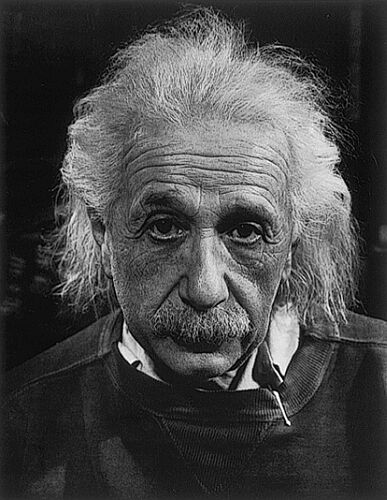
\includegraphics[scale=.2]{Abbildungen/albert-einstein.jpg}
%\vspace*{-5cm}{
%Code ohne Bild:
%\vspace*{-1cm}{
\subsection*{Persönliche Daten}
\flushleft
%\tabular-Umgebung
\normalsize
\begin{tabular}{lcl}
Adresse             & ~ & Albert-Einstein-Straße 98\\
                    & ~ & 91058 Erlangen\\[5pt]
Mobil               & ~ & 0151 - 12345978\\
Email               & ~ & albert@einstein.de\\[5pt]
Geburtsdatum        & ~ & 10.10.1910\\
Staatsangehörigkeit & ~ & deutsch\\
\end{tabular} 

\subsection*{Bachelorarbeit (optionaler Punkt)}
\begin{tabular}{lcl}
01/2016-07/2016     & ~~~~~ & Bachelorarbeit \\
                    & ~~~~~ & Ich bin das Thema der Bachelorarbeit\\[5pt]

\end{tabular} 
\\*  % Zeilenumbruch OHNE Seitenwechsel

\nopagebreak
\subsection*{Studium und Schulbildung}
\begin{tabular}{lcl}
01/2016 - 07/2016     & ~~~ &  Friedrich-Alexander-Universität Erlangen-Nürnberg\\
                      & ~~~ &  Hauptfächer Prokrastination und Bummelei\\
01/2010 - 01/2016     & ~~~ &  Albert-Einstein-Gymnasium, Erlangen\\
                      & ~~~ &  Leistungskurse: Feiern und Relaxen\\
\end{tabular}

\subsection*{Berufliche Erfahrungen / Praktika}
\begin{tabular}{lcl}
01/2016 - 07/2016     & ~~~ &  Wissenschaftlicher Hilfsmitarbeiter am Fraunhofer IIS\\
01/2016 - 07/2016     & ~~~ &  Praktikum bei Siemens Erlangen\\
\end{tabular}
\subsection*{Zusatzqualifikationen - (optional)}
\begin{tabular}{lcl}
Sprachen            &  & Deutsch (Muttersprache)\\
                    &  & Englisch (fließend in Wort und Schrift)\\
                    &  & Französisch (Grundkenntnisse)\\[5pt]
Programmiersprachen &  & Java \\
\end{tabular} 
\bigskip
\vspace*{.5cm}




Erlangen, den (Datum eintragen)\\*[20pt]\nopagebreak
\vspace{0.5cm}


\rule{5cm}{0.4pt}\\*\nopagebreak


Albert Einstein\\*\nopagebreak







\end{document}



 
